

\newpage



%----------------------------------------------------------------------------------------


\section{Spatio-temporal causalities}{Causalités spatio-temporelles}

\label{sec:causalityregimes}

%----------------------------------------------------------------------------------------




%----------------------------------------------

\bpar{This section contributes to the understanding of strongly coupled spatio-temporal processes by describing a generic method based on Granger causality, which is a method introduced in economics to characterize possible causal relationships from correlation relations between variables lagged in time. We indeed introduce here a method allowing to characterize co-evolution at the statistical level.
}{
Cette section contribue à la compréhension des processus spatiotemporels fortement couplés, en proposant une méthode générique basée sur la causalité de Granger, qui est une méthode introduite en économie pour caractériser des possibles relations causales à partir de relations de corrélations entre variables décalées dans le temps. Il s'agit bien ici de l'introduction d'une méthode permettant de caractériser la co-évolution au niveau statistique.
}

\bpar{
The method is validated by the robust identification of causality regimes and of their phase diagram for an urban morphogenesis model that couples network growth with density. The application to the real case of South Africa unveils interactions that change in time, witnessing historical events between territorial demographic dynamics and network growth. 
}{
 Notre méthode est validée par l'identification robuste de régimes de causalité et de leur diagramme de phase pour un modèle de morphogenèse urbaine couplant croissance du réseau et de la densité. L'application au cas réel de l'Afrique du Sud démontre des interactions qui changent dans le temps, témoins des évènements historiques entre les dynamiques démographiques territoriales et la croissance du réseau.
}


\bpar{
The existe in literature a small number of examples using statistical relationships on dynamical relations between network and territories, i.e. trying to establish a causal relationship between the two. For example, \cite{levinson2008density} explains for the case of London population and connectivity to network variables by these same variables lagged in time, unveiling circular causal effects. \cite{doi10.1068/b39089} uses similar techniques for a region in Italy with historical data on long time, but stays moderate on possible conclusions of systematic effects by recalling the importance of historical events on the estimated relations. \cite{cuthbert2005empirical} proceeds to econometric estimations of reciprocal influence, and concludes that in their Canadian case study at a sub-regional scale, the development of the network induces the development of land-use but not the contrary. Space and time scales influence thus significantly the results of such analysis. \cite{koning:hal-00962384} proposes an estimation of relations between the existence of a High Speed Rail connection and economic variables on French Urban Units, and shows a negative effect of the connection itself, after controlling on the endogenous nature of the connection by a selection model, and a significant effect of the characteristics of Urban Units: for example, for urban units benefiting from a TGV connection without LGV, the effect is of -1\% on employments between 1982 and 2006. This study remains however limited as it takes neither a time lag larger than one time step nor spatial relations between entities. Finally, still in the same spirit but without explicit inclusion of space, \cite{MANCMANC1073} shows on long time a causality link between infrastructure stock and economic growth on a global panel, but that these effects are moderated locally by under or over-investments: in that case, macro-economic effects are revealed.
}{
Il existe dans la littérature un petit nombre d'exemples d'utilisation de statistiques spatiales sur les relations dynamiques entre réseaux et territoires, c'est-à-dire cherchant à exhiber des relations de causalité entre les deux. Par exemple, \cite{levinson2008density} explique pour Londres les variations de population et de connectivité au réseau par ces mêmes variables décalées dans le temps, démontrant des effets causaux réciproques. \cite{doi:10.1068/b39089} utilisent des techniques similaires sur une région d'Italie sur des données historiques sur le temps long, mais modère les conclusions en rappelant l'importance des évènements historiques sur les relations estimées. \cite{cuthbert2005empirical} effectuent des estimations économétriques des influences réciproques, et conclut que dans le cas d'étude (au Canada à une échelle régionale) le développement du réseau induit le développement de l'usage du sol, mais pas l'inverse. L'échelle de temps et d'espace devrait logiquement être responsable de cette non-circularité. \cite{koning:hal-00962384} procèdent à une analyse économétrique de la relation entre existence d'une desserte TGV et variables économiques sur les unités urbaines Françaises, et conclut à un effet en propre négatif pour la desserte, après contrôle de l'endogénéité de la desserte par un modèle de sélection, et un effet significatif des caractéristiques propres des unités urbaines : par exemple, pour les unités urbaines desservies par TGV hors LGV, l'effet de la desserte est de -1\% sur les emplois entre 1982 et 2006. Cette étude reste cependant limitée car non spatialisée et prenant en compte un décalage d'une unité de temps seulement. \cite{MANC:MANC1073} montrent sur le temps long un lien de causalité entre stock d'infrastructure et croissance économique sur un panel mondial, mais que ces effets sont atténués localement par des sous ou sur-investissements : dans ce cas, des effets macroéconomiques sont révélés.
%\comment{\cite{carrouet:hal-00980002}}
}

%\comment{\cite{van2014exploring} spatial granger}




%%%%%%%%%%%%%%%
%\subsection[Spatio-temporal Causalities][Causalités Spatio-temporelles]{A method to unveil spatio-temporal causalities}{Une méthode pour identifier des causalités spatio-temporelles}
\subsection{Spatio-temporal causalities}{Causalités spatio-temporelles}


\bpar{The study of strongly coupled spatio-temporal processes implies to understand tangled intrications generally highly difficult to isolate. These interactions are the essence of complexity approaches, and are indeed at the origin of the emergent behavior of the system. They make sense as an object of study in itself and a separation of processes appears then contradictory with an integrated view of the system. In the case of territorial systems, the example of interactions between transportation networks and territories is a good illustration of this phenomenon, as shows the debate on structuring effects developed in chapter~\ref{ch:thematic}. We recall that we have suggested that the reality of territorial processes in in fact much more complicated that a simple causal relationship between the construction of an infrastructure and spillovers on local development, but indeed corresponds to a \emph{co-evolution}. 
}{
L'étude des processus spatio-temporels fortement couplés implique la prise en compte d'imbrications entre ceux-ci généralement difficiles à isoler. Essence même des approches par la complexité, ces interactions qui sont à l'origine du comportement émergent d'un système font sens comme objet d'étude en lui-même, et une séparation des processus paraît alors contradictoire avec une vision intégrée du système. Dans le cas des systèmes territoriaux, l'exemple des interactions entre réseaux de transport et territoires est une bonne illustration de ce phénomène, comme le montre le débat sur les effets structurants développé en chapitre~\ref{ch:thematic}. Nous rappelons que nous avons suggéré que la réalité des processus territoriaux est en fait bien plus compliquée qu'une simple relation causale entre la mise en place d'une infrastructure et les retombées sur le développement local, mais correspond bien à une \emph{co-évolution}.
}

% methods developed in the seventies aimed at isolating the ``structuring effects'' of a transportation infrastructure~\cite{bonnafous1974methodologies} have later been unveiled as a political instrument and with a poor empirical support~\cite{offner1993effets}. The issue is still highly relevant today as it raises for example with the construction of new High Speed Rail lines in France~\cite{crozethalshs01094554}. The reality of territorial processus is in fact much more complicated than a simple causal relation between the introduction of a new infrastructure and spillovers on local development, but corresponds indeed to complex \emph{co-evolutive} processes~\cite{bretagnolletel00459720}. On long time scales and large spatial scales, some effects of dynamics reinforcement in system of cities by the insertion within networks have been shown by the application of the Evolutive Urban Theory~\cite{espacegeo2014effets}, showing that the disentangling is sometimes possible through a more global understanding of the system.
% Le débat est toujours d'actualité puisque la question se pose toujours par exemple pour la construction de lignes à grande vitesse~\cite{crozethalshs01094554}.
%Sur le temps long et à petite échelle, certains effets de renforcement des dynamiques dans les systèmes de villes par l'insertion dans les réseaux, ont été mis en valeur par l'application de la Théorie Evolutive des Villes~\cite{espacegeo2014effets}, montrant que la mise en évidence de régularités est toutefois possible dans certains cas par une compréhension plus globale du système.

\bpar{
At an other scale, still for relations between networks and territories, we can point at the relations between mobility practices, urban sprawl et ressource localisation in a metropolitan framework that are as much complex: \cite{cerqueira2017inegalites} shows for example a strong correspondence between conditioning of mobility practices by the accessibility and socio-professional category.
}{
À une autre échelle, toujours concernant les relations entre réseaux et territoires, on peut citer les liens entre pratiques de mobilité, étalement urbain et localisation des ressources dans un cadre métropolitain qui s'avèrent tout autant complexes : \cite{cerqueira2017inegalites} montre par exemple une forte correspondance entre conditionnement des pratiques de mobilité par l'accessibilité et classe socio-professionnelle.
}

\bpar{
This kind of issue is naturally present in other fields: in Economic Geography, the example of links between innovation, local spillovers of knowledge and aggregation of economic agents is a typical illustration of spatio-temporal economic processes exhibiting circular causalities difficult to disentangle~\cite{audretsch1996r}. Specific methods are introduced, as the use of statistical instruments: \cite{aghion2015innovation} shows that the geographical origin of US Congress members that attribute local subsidies is a powerful instrumental variable to link innovation and income inequalities for higher incomes, what confirms that the significant correlation between the two is indeed a causality of innovation on inequalities\footnote{This example is important from the methodological point of view, but not only since it implicitly links to the thematic of the diffusion of innovation which is crucial in the evolutive urban theory.}.
}{
Ce type de problématique est bien sûr présent dans d'autres domaines : en économie, l'exemple des liens entre innovation, impacts locaux de la connaissance et agrégation des agents économiques est une illustration typiques de processus économiques spatio-temporels présentant des causalités circulaires difficiles à démêler~\cite{audretsch1996r}. Des méthodes spécifiques sont introduites, comme l'utilisation d'instruments statistiques comme par~\cite{aghion2015innovation} dans lequel l'origine géographique des membres du Bureau du Congrès américain attribuant les subventions locales est une bonne variable instrumentale pour lier caractère innovant et inégalités des plus hauts salaires, et permet de montrer que la corrélation significative entre les deux est en fait un lien de causalité dirigé de l'innovation sur les inégalités\footnote{Cet exemple est important sur le plan méthodologique, mais pas seulement puisqu'il se lie en filigrane au thème de la diffusion de l'innovation qui est crucial dans la théorie évolutive des villes.}.
}

\subsubsection{Causality in geography}{Causalité en géographie}

\bpar{
Strong coupling in space and time generally implies a notion of causality, that geography has always studied: \cite{loi1985etude} shows that fundamental issues tackled by contemporary theoretical geography (isolation of objects, link between space and causal structures, etc.) were already implicit in \noun{Vidal}'s classical geography.
}{
Le couplage fort spatio-temporel implique généralement l'introduction de la notion de causalité, à laquelle la géographie s'est toujours intéressée : \cite{loi1985etude} montre que les questions fondamentales que se pose la géographie théorique récente (isolation des objects, lien entre espace et structures causales, etc.) étaient déjà présentes dans la géographie classique de \noun{Vidal}.
}


\bpar{
Beside, \cite{claval1985causalite} criticizes the new determinisms having emerged, in particular the one advocated by some scholars of systemic analysis\footnote{See~\cite{chamussy1984dynamique} for an example of model with a planning purpose positioned within that research stream.}: in its beginning, this approach inherited from cybernetics and thus of a reductionist vision implying a determinism even for a probabilistic formulation. \noun{Claval} observes that works contemporary to his writings could allow to capture the complexity that characterizes human decisions: the Prigogine School and the Theory of Catastrophes by René Thom.
}{
\cite{claval1985causalite} critique d'ailleurs les nouveaux déterminismes ayant émergé, notamment celui proposé par certains tenants de l'analyse systémique\footnote{Voir~\cite{chamussy1984dynamique} pour un exemple de modèle à but de planification se plaçant dans ce courant.} : dans ses débuts, cette approche héritait de la cybernétique et donc d'une vision réductionniste impliquant un déterminisme même dans une formulation probabiliste. \noun{Claval} note que des travaux contemporains à son écriture (l'école de Prigogine et la Théorie des Catastrophes de Thom) devraient permettre de capturer la complexité qui fait la particularité des décisions humaines.
}



\bpar{
This viewpoint has anticipated posterior developments, since as Pumain recalls in~\cite{pumain2003approche}, the shift from system analysis to self-organisation and complexity has been long and progressive, and these works have played a fundamental role for it. \noun{François Durand-Dastès} sums up this picture more recently in~\cite{durand2003geographes}, by focusing on the importance of bifurcations and path-dependency in the initial moments of the constitution of a system that he defines as \emph{systemogenesis}\footnote{This notion can be put closer to the one of \emph{morphogenesis} that we study more deeply in chapter~\ref{ch:morphogenesis}.}. This type of complex dynamics generally implies a co-evolution of system components, that can be understood as circular causalities between processes: the issue of identifying them is thus crucial regarding the notion of causality for contemporary complex geography.
}{
Ce point de vue a anticipé les développements antérieurs, puisque comme le rappelle~\cite{pumain2003approche}, le glissement de l'analyse des systèmes à l'auto-organisation puis à la complexité a été long et progressif, et ces travaux ont été fondamentaux pour le permettre. \noun{François Durand-Dastès} résume cette situation plus récemment dans \cite{durand2003geographes}, en appuyant l'importance des bifurcations et de la dépendance au chemin lors des instants initiaux de la constitution du système qu'il désigne par \emph{systèmogenèse}\footnote{Cette notion peut être rapprochée de celle de \emph{morphogenèse} que nous approfondissons en chapitre~\ref{ch:morphogenesis}.}. Ce type de dynamique complexe implique généralement une co-évolution des composantes du système, qu'on peut interpréter comme des causalités circulaires entre processus : la question de pouvoir les identifier est donc cruciale au regard de la notion de causalité pour la géographie complexe contemporaine.
}


\bpar{
This view of a complex causality~\cite{morin1976methode} can also be put into perspective with the concept of \emph{cumulative causality} in economics~\cite{skott1995cumulative}, which insists on the role of path-dependency and the possibility for small perturbations to cause significant effects by negative feedback: it is then impossible to separate the effects from their causes in infinitesimal perturbations.
}{
Cette vision d'une causalité complexe~\cite{morin1976methode} peut être aussi mise en perspective avec le concept de \emph{causalité cumulative} en économie~\cite{skott1995cumulative}, qui insiste sur le rôle de la dépendance au chemin et la possibilité pour de petites perturbations de causer des effets conséquents par rétroaction négative : il est alors impossible de séparer les effets des causes dans les perturbations infinitésimales.
}



%\comment{micro-macro ; lien avec morphogenese ; equifinalité.}

% remarque de Seb : il faut que tu précises que tu parle des géographes francais, car l'introduction du projet systémique varie selon les pays et les branches de la géographie. Chorley par exemple à introduit très tôt les concepts de systèmes ouverts de bertalanffy en géographie physique. Varenne a écrit un papier la dessus en 2014 également.

% https://scholar.google.fr/scholar?hl=fr&as_sdt=0%2C5&q=cumulative+causation&btnG=

% note on systemogenesis : here we could introduce morphogenesis, form as system structure, linked to circular causalities ; topology and dynamical systems in network propagation (paper Nature Networks). Too far, but keep in mind for further work ?


\subsubsection{Identification of causalities}{Identification de causalités}


%%%%%%
%% -- TRAD --
%%%%%%



\bpar{
The regimes under which identification of causalities are relevant are not obviously known. These will depend of the definitions used, as well as available methods for which we give now a few examples. \cite{liu2011discovering} proposes to detect spatio-temporal relations between perturbations of trafic flows, introducing a particular definition of causality based on correspondance of extreme points. Associated algorithms are however specific and difficult to apply to other kind of systems. The use of spatio-temporal correlations has been shown to have in some cases a strong predictive power for trafic flows~\cite{min2011real}. Also in the field of transportation and land-use, \cite{xie2009streetcars} applies a Granger causality analysis, that can be interpreted as lagged correlation, to show for a case study that network growth inducts urban development and is itself driven by externalities such as mobility habits.
}{
Le caractère opérationnel de l'identification des causalités peut prendre des formes très diverses, dans différents domaines. Celui-ci dépendra des définitions utilisées, de la même manière que des méthodes à disposition pour lesquelles nous pouvons donner quelques illustrations, en essayant de s'intéresser à des champs divers pour mettre en valeur les différents enjeux et possibilités méthodologiques. \cite{goudet2017learning} utilisent des réseaux de neurones pour inférer des relations de causalité entre variables au sens des probabilités conditionnelles. \cite{liu2011discovering} proposent la détection de relations spatio-temporelles entre perturbations des flux de trafic, introduisant une définition particulière de la causalité basée sur une correspondance de points extrêmes. Les algorithmes associés sont toutefois spécifiques et difficilement applicables à des types de systèmes différents. L'utilisation des corrélations spatio-temporelles a été démontrée comme ayant dans certains cas un fort pouvoir prédictif pour les flux de traffic~\cite{min2011real}. Également dans le domaine des transports et de l'usage du sol, \cite{xie2009streetcars} appliquent une analyse par causalité de Granger, qu'on pourra interpréter comme une corrélation retardée, pour montrer dans un cas particulier que la croissance du réseau induit le développement urbain et est elle-même tirée par des externalités comme les habitudes de mobilité.
}


\bpar{
Neuroscience has developed numerous methods answering similar issues. \cite{luo2013spatio} defines a generalized Granger causality that takes into account non-stationarity and applies to abstracts regions produced by functional imaging. This kind of method is also developed in Computer Vision, as illustrated by \cite{ke2007spatio} that exploits spatio-temporal correlations of forms and flows between successive images to classify and recognize actions. Applications can be quite concrete such as compression of video files by extrapolation of motion vectors~\cite{chalidabhongse1997fast}. In all these cases, the study of spatio-temporal correlations meets the weak notions of causality described above.
}{
Les neurosciences ont développé de nombreuses méthodes répondant à des problématiques similaires. \cite{luo2013spatio} définissent une causalité de Granger généralisée prenant en compte la non-stationnarité et s'appliquant à des régions abstraites issues d'imagerie fonctionnelle. Ce genre de méthode est également développée en Vision par Ordinateur, comme l'illustrent \cite{ke2007spatio} qui exploitent les corrélations spatio-temporelles de formes et de flux dans des successions d'images pour classifier et reconnaître des actions. Les applications peuvent être très concrètes comme la compression de fichiers videos par extrapolation des vecteurs de mouvement~\cite{chalidabhongse1997fast}. Dans l'ensemble de ces cas, l'étude des corrélations spatio-temporelles rejoint la plupart des notions faibles de causalité vues précédemment, au sens d'une relation de corrélation entre variables dans le temps et l'espace. Ces mesures de causalité sont plus proches de la ``causalité prédicative'' en opposition à la causalité ``stimulus-réponse'' comme indiqué par \cite{bonnafous:halshs-00291521} (p.~90), mais permettent une grande flexibilité de mise en pratique.
}


\bpar{
This contribution aims to explore the possibility of a similar methods for spatio-temporal data exhibiting a priori complex circular causalities, and thus to realize the difficult exercise to couple a certain level of simplicity with a grasping of complexity. We introduce therefore a method to analyse spatio-temporal correlations, similar to a Granger causality estimated in space and time. The robustness of the method is demonstrated in a systematic way by the application to a complex model of simulation of urban morphogenesis, what leads to the unveiling of distinct causality regimes in the phase space of the model. We also include the application to an empirical case study, what positions this work at the interface between knowledge domains of methodology, modeling and empirical within the epistemological framework introduced by~\cite{2017arXiv170609244R}.
}{
Nous cherchons ici à explorer la possibilité d'une méthode analogue pour des données spatio-temporelles présentant a priori des causalités circulaires complexes, et donc de tenter de concilier un certain niveau de simplicité et de caractère opérationnel à une prise en compte de la complexité. Nous introduisons ainsi une méthode d'analyse des corrélations spatio-temporelles similaire à une causalité de Granger estimée dans le temps et l'espace, dont la robustesse est démontrée par l'application systématique à un modèle de simulation complexe de morphogenèse urbaine et par l'isolation de régimes de causalités distincts dans l'espace des phases du modèle. Notre contribution inclut également l'application à un cas d'étude empirique, ce qui la positionne à l'interface des domaines de la méthodologie, de la modélisation et de l'empirique.
}



\bpar{
The rest of this section is organized as follows: the generic framework of the method is described in the next section. We then apply it to a synthetic dataset to partially validate it and test its potentialities, what allows us to apply it then to the real case study of Grand Paris transportation network. We finally discuss to proximity with existing methods and possible developments.
}{
La suite de cette section est organisée de la façon suivante : le cadre générique de la méthode proposée est décrit. Nous l'appliquons ensuite à un jeu de données synthétiques afin de la valider partiellement et de tester ses potentialités, ce qui permet de l'appliquer ensuite au système urbain sud-Africain sur le temps long. Nous discutons finalement la proximité avec d'autres méthodes existantes et des développements possibles.
}



%%%%%%%%%%%%%%%
\subsubsection{Method}{Méthode}
%%%%%%%%%%%%%%%


\bpar{
We formalize here the method in a generic way, based in a weak formulation of Granger causality, to try to identify causal relations in spatial systems. Let $X_j(\vec{x},t)$ spatio-temporal unidimensional random processes, which realizations occur in space and time. We give a set of fundamental spatial units  $(u_i)$ that can be for example raster cells or any paving of the geographical space. We assume the existence of functions $\Phi_{i,j}$ allowing to make the correspondance between the realization of each components and spatial units, possibly through a first spatial aggregation or by a more elaborated process driven by a network for example. A realization of a system is given by a set of trajectories for each process $x_{i,j,t}$, and we write a set of realizations $x^{(k)}_{i,j,t}$ (accessible by stochastic repetitions in the case of a model of simulation for example, or by assumption of comparability of territorial sub-systems in real cases). We assume to have a correlation estimator $\hat{\rho}$ applying in time, space and repetitions, i.e. $\hat{\rho}\left[X,Y\right] = \hat{\mathbb{E}}_{i,t,k}\left[XY\right] - \hat{\mathbb{E}}_{i,t,k}\left[X\right]\hat{\mathbb{E}}_{i,t,k}\left[Y\right]$. 
}{
Nous formalisons ici de manière générique la méthode, basée sur un test similaire à la causalité de Granger\footnote{On rappelle que la causalité de Granger correspond à l'existence d'une relation significative entre les composantes retardées dans le temps d'un vecteur et celui-ci.}, pour tenter d'identifier des relations causales dans des systèmes spatiaux. Soit $X_j(\vec{x},t)$ des processus aléatoires spatiaux unidimensionnels, se réalisant dans le temps et l'espace. On se donne un ensemble d'unités spatiales fondamentales $(u_i)$ qui peuvent être par exemple les cellules d'une image raster ou un pavage quelconque de l'espace géographique\footnote{Mais dont le choix sera à faire soigneusement, en lien avec la thématique étudiée, notre méthode n'échappant a priori pas au problème du \emph{MAUP}~\cite{paez2005spatial}.}. On suppose l'existence de fonctions $\Phi_{i,j}$ permettant de faire correspondre les réalisations de chaque composante aux unités spatiales, possiblement par une première agrégation locale. Une réalisation d'un système est donnée par un ensemble de trajectoires pour chaque processus $x_{i,j,t}$, et on pourra noter un ensemble de réalisations $x^{(k)}_{i,j,t}$ (accessibles dans le cas d'un modèle de simulation par exemple, ou par hypothèse de comparabilité de sous-systèmes territoriaux dans des cas réels). On suppose disposer d'un estimateur de corrélation $\hat{\rho}$ s'exerçant dans le temps, l'espace et les répétitions, c'est-à-dire que la covariance est estimée\footnote{L'estimateur $\hat{\mathbb{E}}$ portant ici sur le temps $t$, les unités spatiales $i$ et les répétitions $k$.} par
}

\[
\hat{\Cov}\left[X,Y\right] = \hat{\mathbb{E}}_{i,t,k}\left[XY\right] - \hat{\mathbb{E}}_{i,t,k}\left[X\right]\hat{\mathbb{E}}_{i,t,k}\left[Y\right]
\]
%TODO : rq : did precise somewhere which estimator of covariance ? -> use of the biased one in NetLogo / unbiased one in R ==> implementation bias somehow.

\bpar{
It is important to note here the hypothesis of spatial and temporal stationarity, that can however easily be relaxed in the case of local stationarity. 
}{
Il est important de noter ici l'hypothèse de stationnarité spatiale et temporelle, qui peut toutefois aisément être relaxée dans le cas d'une stationnarité locale : il s'agira dans un tel cas d'estimer sur des fenêtres spatiales ou temporelles glissantes.
}

\bpar{
Furthermore, spatial auto-correlation is not explicitly included, but is taken into account either by the initial spatial aggregation is the characteristic scale of units is larger than the one of neighborhood effects, either by an adequate spatial estimator (weighted spatial statistics of type \emph{GWR}~\cite{brunsdon1998geographically} for example). It allows us to define the lagged correlation by 
}{
D'autre part, l'auto-corrélation spatiale n'est pas explicitement incluse, mais est prise en compte soit par l'agrégation initiale si l'échelle caractéristique des unités est plus grande que celle des effets de voisinage, soit par un estimateur spatial adéquat (statistiques spatiales pondérées de type \emph{GWR}\footnote{On rappelle que la Regression Géographique Pondérée consiste à estimer des modèles statistiques à différents endroits de l'espace, en pondérant les informations par la distance, c'est-à-dire en d'autre termes de prendre en compte la non-stationnarité spatiale.}~\cite{brunsdon1998geographically} par exemple). Cela nous permet de définir la correlation retardée entre les composantes $X_{j_1}$ et $X_{j_2}$ pour le délai $\tau$ par
}


%\comment[FL]{estimateur de correlation : sens ?}

\begin{equation}
\rho_{\tau}\left[X_{j_1},X_{j_2}\right] = \hat{\rho}\left[x^{(k)}_{i,j_1,t - \tau},x^{(k)}_{i,j_2,t}\right]
\end{equation}



\bpar{
The lagged correlation is not symmetric, but we have directly $\rho_{\tau}\left[X_{j_1},X_{j_2}\right] = \rho_{-\tau}\left[X_{j_2},X_{j_1}\right]$. This measure is applied in a simple way: if $\textrm{argmax}_{\tau} \rho_{\tau}\left[X_{j_1},X_{j_2}\right]$ or $\textrm{argmin}_{\tau} \rho_{\tau}\left[X_{j_1},X_{j_2}\right]$ are ``clearly defined'' (both could be simultaneously), their sign will give the sense of causality between components $j_1$ and $j_2$ and their absolute value the propagation lag.
}{
La corrélation retardée n'est pas directement symétrique, mais on a de manière évidente $\rho_{\tau}\left[X_{j_1},X_{j_2}\right] = \rho_{-\tau}\left[X_{j_2},X_{j_1}\right]$. On applique alors cette mesure de manière simple : si $\textrm{argmax}_{\tau} \rho_{\tau}\left[X_{j_1},X_{j_2}\right]$ ou $\textrm{argmin}_{\tau} \rho_{\tau}\left[X_{j_1},X_{j_2}\right]$ sont ``clairement définis'' (les deux pouvant l'être simultanément), leur signe donnera alors le sens de la causalité entre les composantes $j_1$ et $j_2$ et leur valeur absolue le retard de propagation.
}

Par exemple, $X_{j_1}$ pourra être une propriété liée au réseau comme la centralité de proximité, et $X_{j_2}$ une propriété liée aux territoires, comme la densité de population. Cette mesure permettra alors de déterminer un sens de causalité (éventuellement réciproque) entre ces propriétés. Le retard $\tau$ sera typiquement un certain nombre d'années, en association avec l'échelle spatiale des unités d'estimation qui pourra varier de l'échelle du quartier à celle des aires urbaines, comme nous le verrons dans les différents cas d'application par la suite.


\bpar{
The criteria for significance will depend on the case of application and of the estimator used, but can for example include the significance of the statistical test (Fisher test in the case of a Pearson estimator), the position of extremities of a confidence interval of a given level, or even an exogenous threshold $\theta$ on $\left|\rho_{\tau}\right|$ to ensure a certain level of correlation.
}{
Les critères de significativité dépendront du cas d'application et de l'estimateur utilisé. Ils peuvent prendre en compte différents aspects de la robustesse de l'estimation. Par exemple, un filtrage sur la significativité du test statistique (test de Fisher dans le cas d'un estimateur de Pearson) permet de s'assurer d'isoler des relations qui sont statistiquement significatives. On peut aussi vouloir s'assurer de la significativité d'une corrélation minimale, et regarder la position des bornes d'un intervalle de confiance à un niveau donné. Enfin, on peut aussi fixer un seuil exogène $\theta$ sur $\left|\rho_{\tau}\right|$ pour forcer un certain degré de corrélation.
}


\bpar{

}{
Pour résumer la structure de la méthode et l'enchainement des traitements effectués, nous proposons le schéma dans l'Encadré~\ref{frame:causalityregimes:regimes} ci-dessous. La méthode que nous proposons n'est pas nouvelle dans les éléments utilisés, mais l'enchaînement des différentes étapes est originale.
}


%%%%%%%%%%%%%
\begin{figure}[h!]
\begin{mdframed}
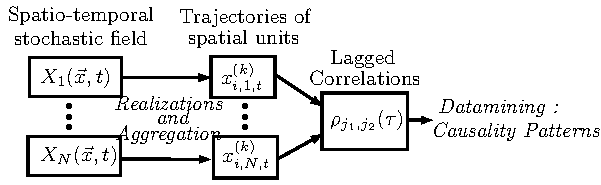
\includegraphics[width=\textwidth]{Figures/Theory/causality_regimes}
\medskip
\framecaption{\textbf{Structure of the methodology.}\label{frame:causalityregimes:regimes}}{\textbf{Structure de la méthodologie.} Nous partons d'un champ stochastique dans le temps et l'espace $X_j(\vec{x},t)$. Un certain nombre de ses réalisations sont capturées, et mesurées sur des unités spatiales. Nous obtenons des trajectoires $k$ par unité $i$ dans le temps $t$, notées $x_{i,j,t}^{(k)}$, sur lesquelles la matrice des corrélations retardées $\rho_{j_1,j_2}(\tau)$ est estimée. Le datamining sur celles-ci permet d'établir différents \emph{régimes de causalité}. \label{frame:causalityregimes:regimes}}
\end{mdframed}
\end{figure}
%%%%%%%%%%%%%


Avant de nous plonger dans l'exploration empirique de la méthode, donnons-en une vision intuitive pour mieux comprendre son lien avec la co-évolution. L'encadré~\ref{frame:causalityregimes:twovars} synthétise des situation stylisées pouvant se produire dans le cas de deux variables. De manière caricaturale, avec deux variables $X,Y$, le profil de $\rho_{\tau}\left[X,Y\right]$ est traduit selon les caractéristiques suivantes : existence d'un extremum ou non pour $\tau < 0$ et existence d'un extremum ou non pour $\tau > 0$, c'est-à-dire possibilités de causalité de $X$ vers $Y$ et/ou de causalité de $Y$ vers $X$. Nous illustrons quatre exemples de profils et représentons les interactions entre variables sous forme graphique, dans le temps et de manière synthétique. 



%%%%%%%%%%%%%
\begin{figure}[h!]
\begin{mdframed}
\bigskip
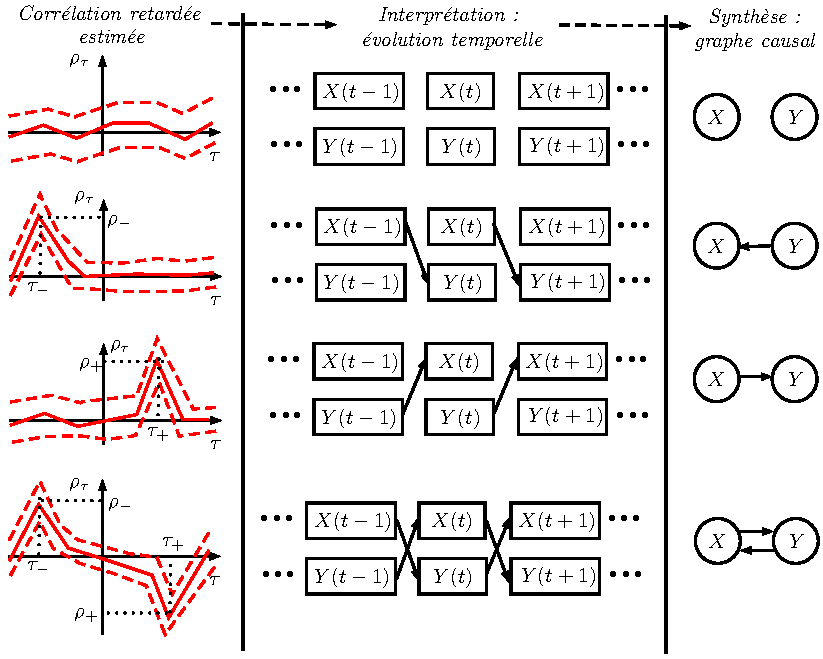
\includegraphics[width=\textwidth]{Figures/Theory/causality_twovars}
\bigskip
\framecaption{\textbf{Illustration of possible configurations in the case of two variables.}\label{frame:causalityregimes:twovars}}{\textbf{Illustration de situations possibles dans le cas de deux variables.} Pour simplifier, nous ne différencions les situations que par l'existence ou non d'un extremum pour les valeurs positives et négatives du délai $\tau$ (et ne prenons pas en compte le signe de la corrélation correspondante). Les lignes pointillées illustrent un seuil de significativité, par exemple un intervalle de confiance sur la corrélation estimée. On a donc quatre situations : aucun extremum significatif, existence de $\tau_-$, existence de $\tau_+$ et existence de $\tau_-$ et de $\tau_+$. Dans le premier, il n'y a pas de lien diachronique entre les variables (mais possiblement des corrélations simultanées, spécifiées par les doubles flèches verticales). Dans les deux suivants, l'une ``cause'' l'autre variable (nous utiliserons parfois ce raccourci sémantique pour commenter les résultats des analyses). Enfin dans la dernière, on a causalités circulaires : de tels motifs s'apparenteront à ce que l'on désignait conceptuellement par co-évolution.\label{frame:causalityregimes:twovars}}
\end{mdframed}
\end{figure}
%%%%%%%%%%%%%

%\comment{voir aussi réseau bayesiens, semble proche de l'idee de reseaux entre variables}



\subsubsection{Emergence and a proxy to measure co-evolution ?}{Emergence et mesure de la co-évolution ?}


% idee sur les repets : lors de l'agreg perd de l'information ? lie au maup..

Prenons également un court instant pour clarifier le statut épistémologique et ontologique attendu par l'application de cette méthode, et dans quelle mesure on peut espérer l'utiliser comme mesure indirecte de la co-évolution. La causalité de Granger est estimée à la fois \emph{dans le temps}, \emph{dans l'espace} et \emph{entre les répétitions}. Dans le cas où l'on observe un phénomène historique, on a une unique trajectoire et l'estimation est faite dans le temps et l'espace uniquement, mais dans tous les cas on passe de caractéristiques à l'échelle microscopique à une mesure macroscopique\footnote{Nous utilisons ici ces termes pour simplifier, il s'agit en fait d'un échelle donnée à une échelle supérieure qui dépend de l'étendue temporelle et spatiale totale.}. Ainsi, on peut avoir des interactions microscopiques circulaires, mais émergence d'un sens de la causalité au niveau macroscopique, ou l'inverse. Rejoignant la question des populations et individus pour la définition de la co-évolution en biologie (voir~\ref{sec:epistemology}), pour laquelle les adaptations mutuelles émergent au niveau des espèces, nous postulons que la caractérisation des motifs de causalité est une manière de caractériser des dynamiques co-évolutives pour les systèmes territoriaux, correspondant alors à notre définition intermédiaire de la co-évolution au niveau d'une population.


Est-il alors possible de répondre de manière équivoque à la question ``\textit{y a-t-il co-évolution dans un cas particulier}''\footnote{A laquelle nous ajoutons : pour ces composantes, sur cette portée spatiale et temporelle et sur ces échelles spatiale et temporelle.} ? Cela se saurait si nous pouvions réinventer l'eau chaude mais qui se chauffe elle-même. Nous voulons dire par là, et nous le verrons dans les multiples développements, que de nombreux problèmes fondamentaux intrinsèques à l'étude des systèmes géographiques (la question des échelles, de la définition du système, des variables prises en compte, le problème de l'observation de trajectoire uniques, de données bruitées et éparses, le problème du MAUP, etc.) seront bien toujours présents, et que la question ci-dessus qui y est naturellement soumise s'avère naïve. Mais nous verrons qu'il sera bien possible d'isoler des signaux clairs, et mettrons en évidence des cas où il existe un sens causal et d'autres où il y a circularité au niveau macroscopique.

% -> en conclusion partie II, revenir la dessus et preciser/clarifier la co-evol conceptuelle et la co-evol ``empirique'', enfin son proxy.



%%%%%%%%%%%%%%%
\subsection{Synthetic data}{Données Synthétiques}

Nous explorons et validons la méthode dans un premier temps sur données synthétiques, c'est-à-dire générées par l'intermédiaire d'un modèle avec un certain niveau de contrôle.


\subsubsection{Auto-regressive time series}{Séries temporelles auto-régressives}

Illustrons les motifs qui peuvent être attendus, notamment ceux stylisés donnés précédemment en Encadré~\ref{frame:causalityregimes:twovars}, sur des données synthétiques avec une structure simple. L'idée est de générer des séries temporelles sur lesquelles le retard et le niveau de corrélation sont contrôlés, ainsi que les résultats théoriques connus.


Soit $\vec{X}(t)$ un processus stochastique suivant l'équation d'auto-régression $\vec{X}(t) = \sum_{\tau > 0} \mathbf{A}(\tau) \cdot \vec{X}(t - \tau ) + \vec{\epsilon}(t)$. Dans le cas où $\mathbf{A}(\tau) = 0$ pour $\tau \neq \tau_0$ et $\mathbf{A}(\tau_0) = \left( {\begin{array}{cc} 0 & a \\ a & 0 \\ \end{array}} \right)$ pour $-1<a<1$, le calcul des corrélations théoriques est possible (voir Annexe~\ref{app:sec:causalityregimes}), et on obtient, en notant $\mathbf{X} = (X,Y)$, pour $\tau > 0$
\[
\rho\left[X(t),Y(t-\tau)\right] = \begin{cases}
	a^{2k+1} \textrm{si } \tau = (2k+1)\tau_0\textrm{ pour tout }k\in \mathbb{Z} \\
	0 \textrm{ sinon} 
\end{cases}
\]

L'expression est la même pour $\tau<0$ en échangeant $X$ et $Y$. Ainsi, on contrôle la corrélation retardée au retard voulu et aux retards qui en sont multiples avec un facteur impair. En changeant l'un des coefficients en 0 ou en son opposé, on obtient pour les premiers maximums les trois profils stylisés donnés en Encadré~\ref{frame:causalityregimes:twovars}.


Utilisons cet exemple pour explorer numériquement la possibilité de classifier les profils de corrélations retardées. Nous considérons le même processus pour $\tau_0 = 2$ et $\mathbf{A}(\tau_0) = \left( {\begin{array}{cc} 0 & a_1 \\ a_2 & 0 \\ \end{array}} \right)$, avec $-1<a_1,a_2<1$. Nous simulons avec ce modèle des séries temporelles de longueur $t_f=10000$ en tirant $b=10000$ valeurs aléatoires pour les paramètres $(a_1,a_2)$. Sur chaque série les corrélations retardées sont estimées, et nous procédons à une classification non-supervisée\footnote{Par algorithme des \emph{k-means} avec $k=9$ et $b_c = 1000$ répétitions.} sur les séries temporelles $\left[\rho(\tau)\right]_{a_1,a_2}$. Nous montrons en Fig.~\ref{fig:causalityregimes:arma} les profils typiques obtenus en correspondance avec leur position dans l'espace des paramètres $(a_1,a_2)$. Nous obtenons exactement les neuf profils stylisés possibles, en correspondance avec les valeurs relatives des paramètres comme attendu. À partir de profils très variés de corrélations retardées, nous sommes ainsi capable d'extraire des profils typiques d'interaction entre les variables. Cela nous renforce dans l'idée d'appliquer cette méthode sur des données plus complexes par la suite.


% comparaison correlation theorique / correlation empirique
% -> pas besoin, evident pour des ts seules. on pourrait estimer la valeur pour le centre du cluster ? pas si evident.

%%%%%%%%%%%%%
\begin{figure}
	%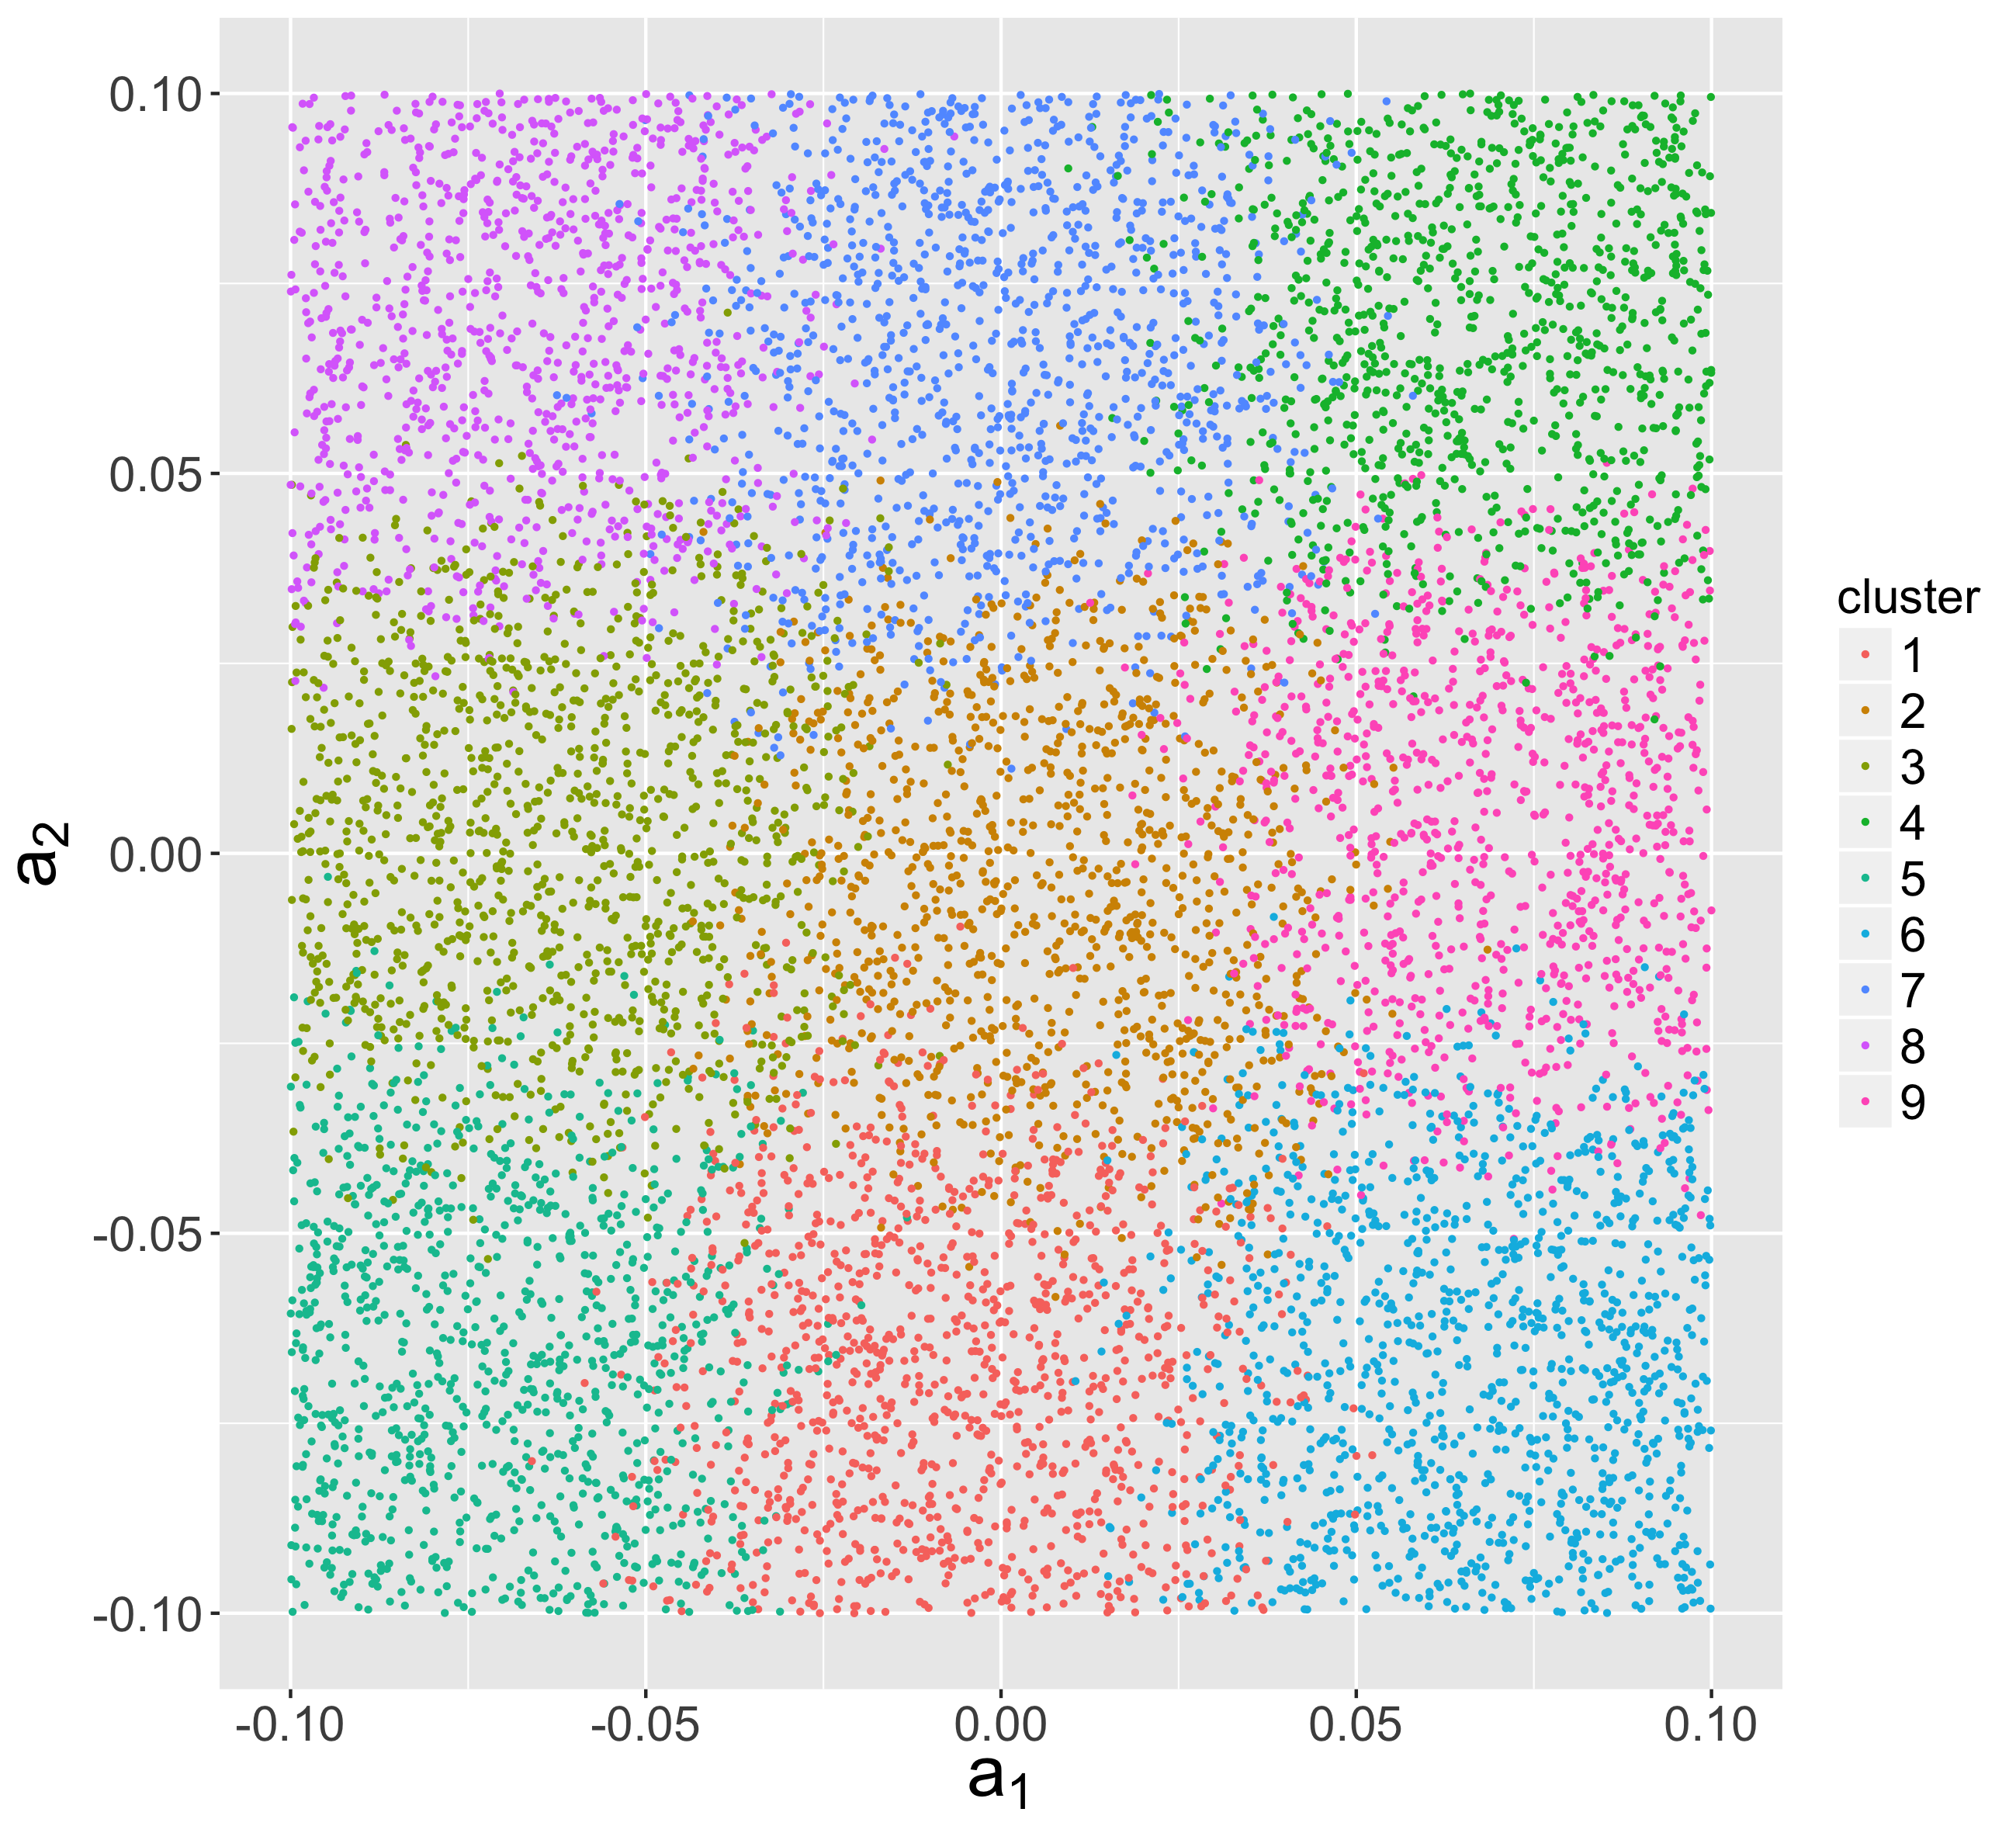
\includegraphics[width=0.48\linewidth]{Figures/CausalityRegimes/coefsclust_nbootstrap10000_maxai0_1_lag2nclust9.png}
	%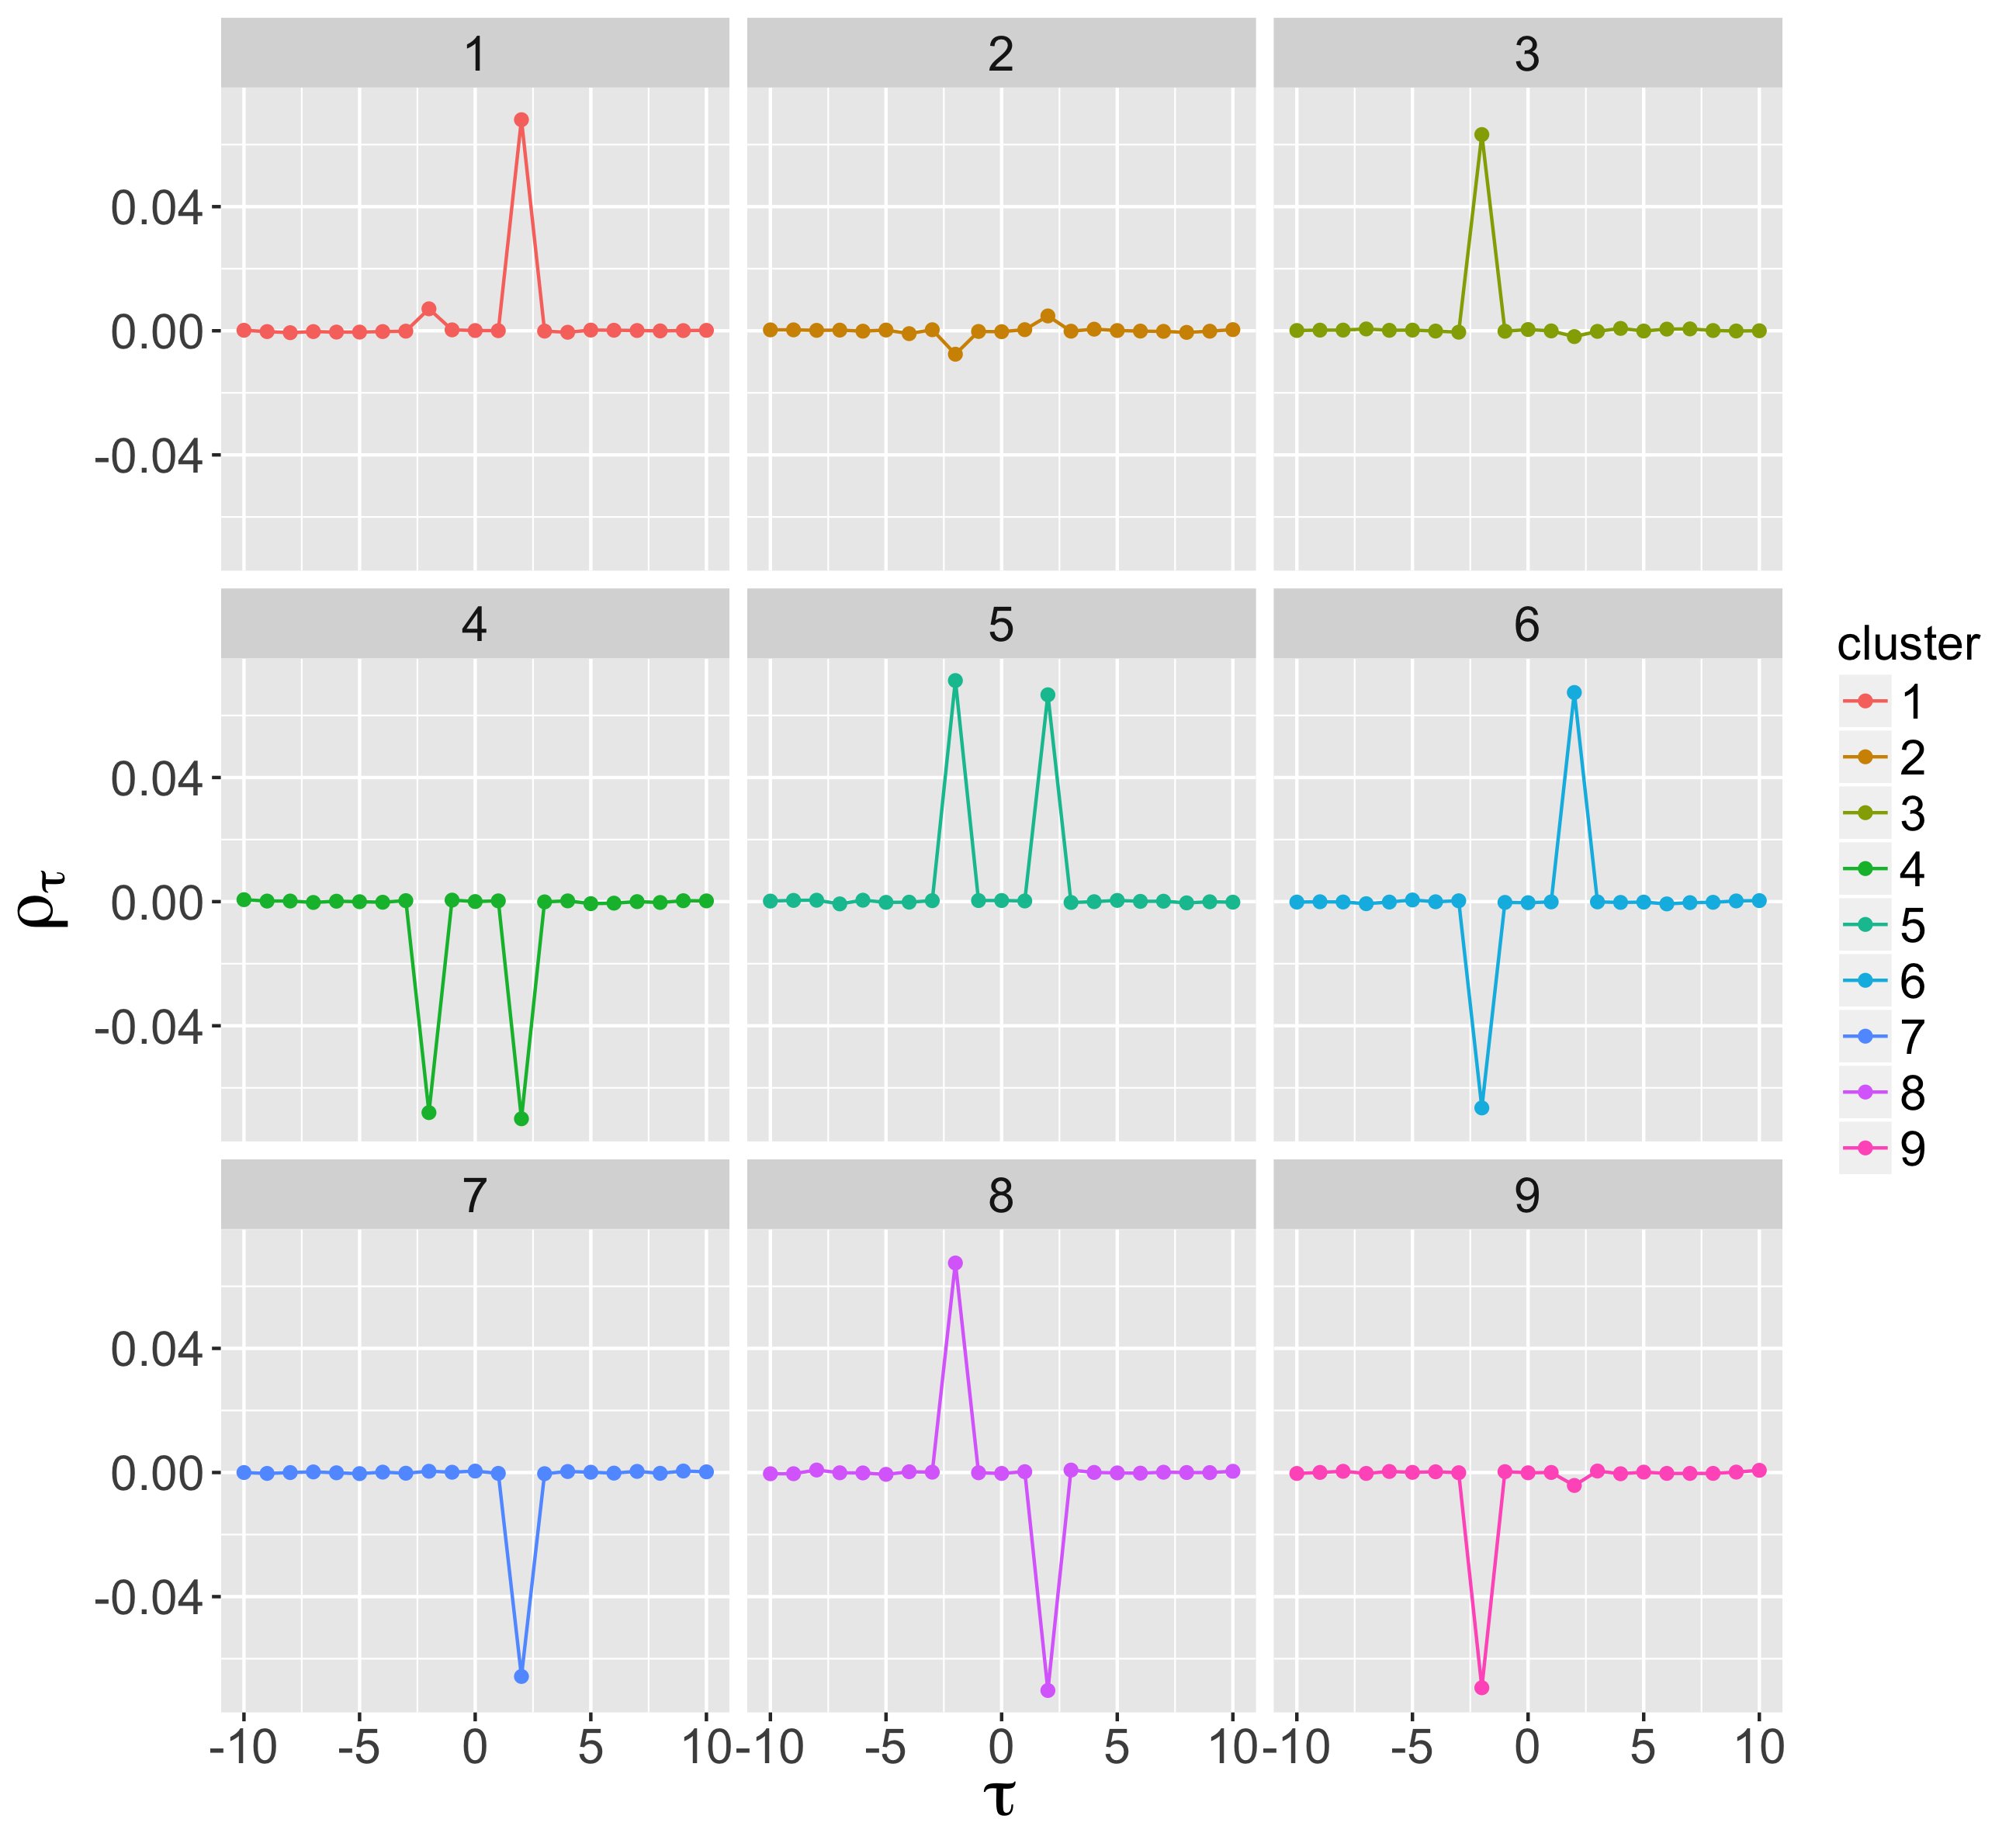
\includegraphics[width=0.48\linewidth]{Figures/CausalityRegimes/centertrajs_nbootstrap10000_maxai0_1_lag2nclust9.png}
	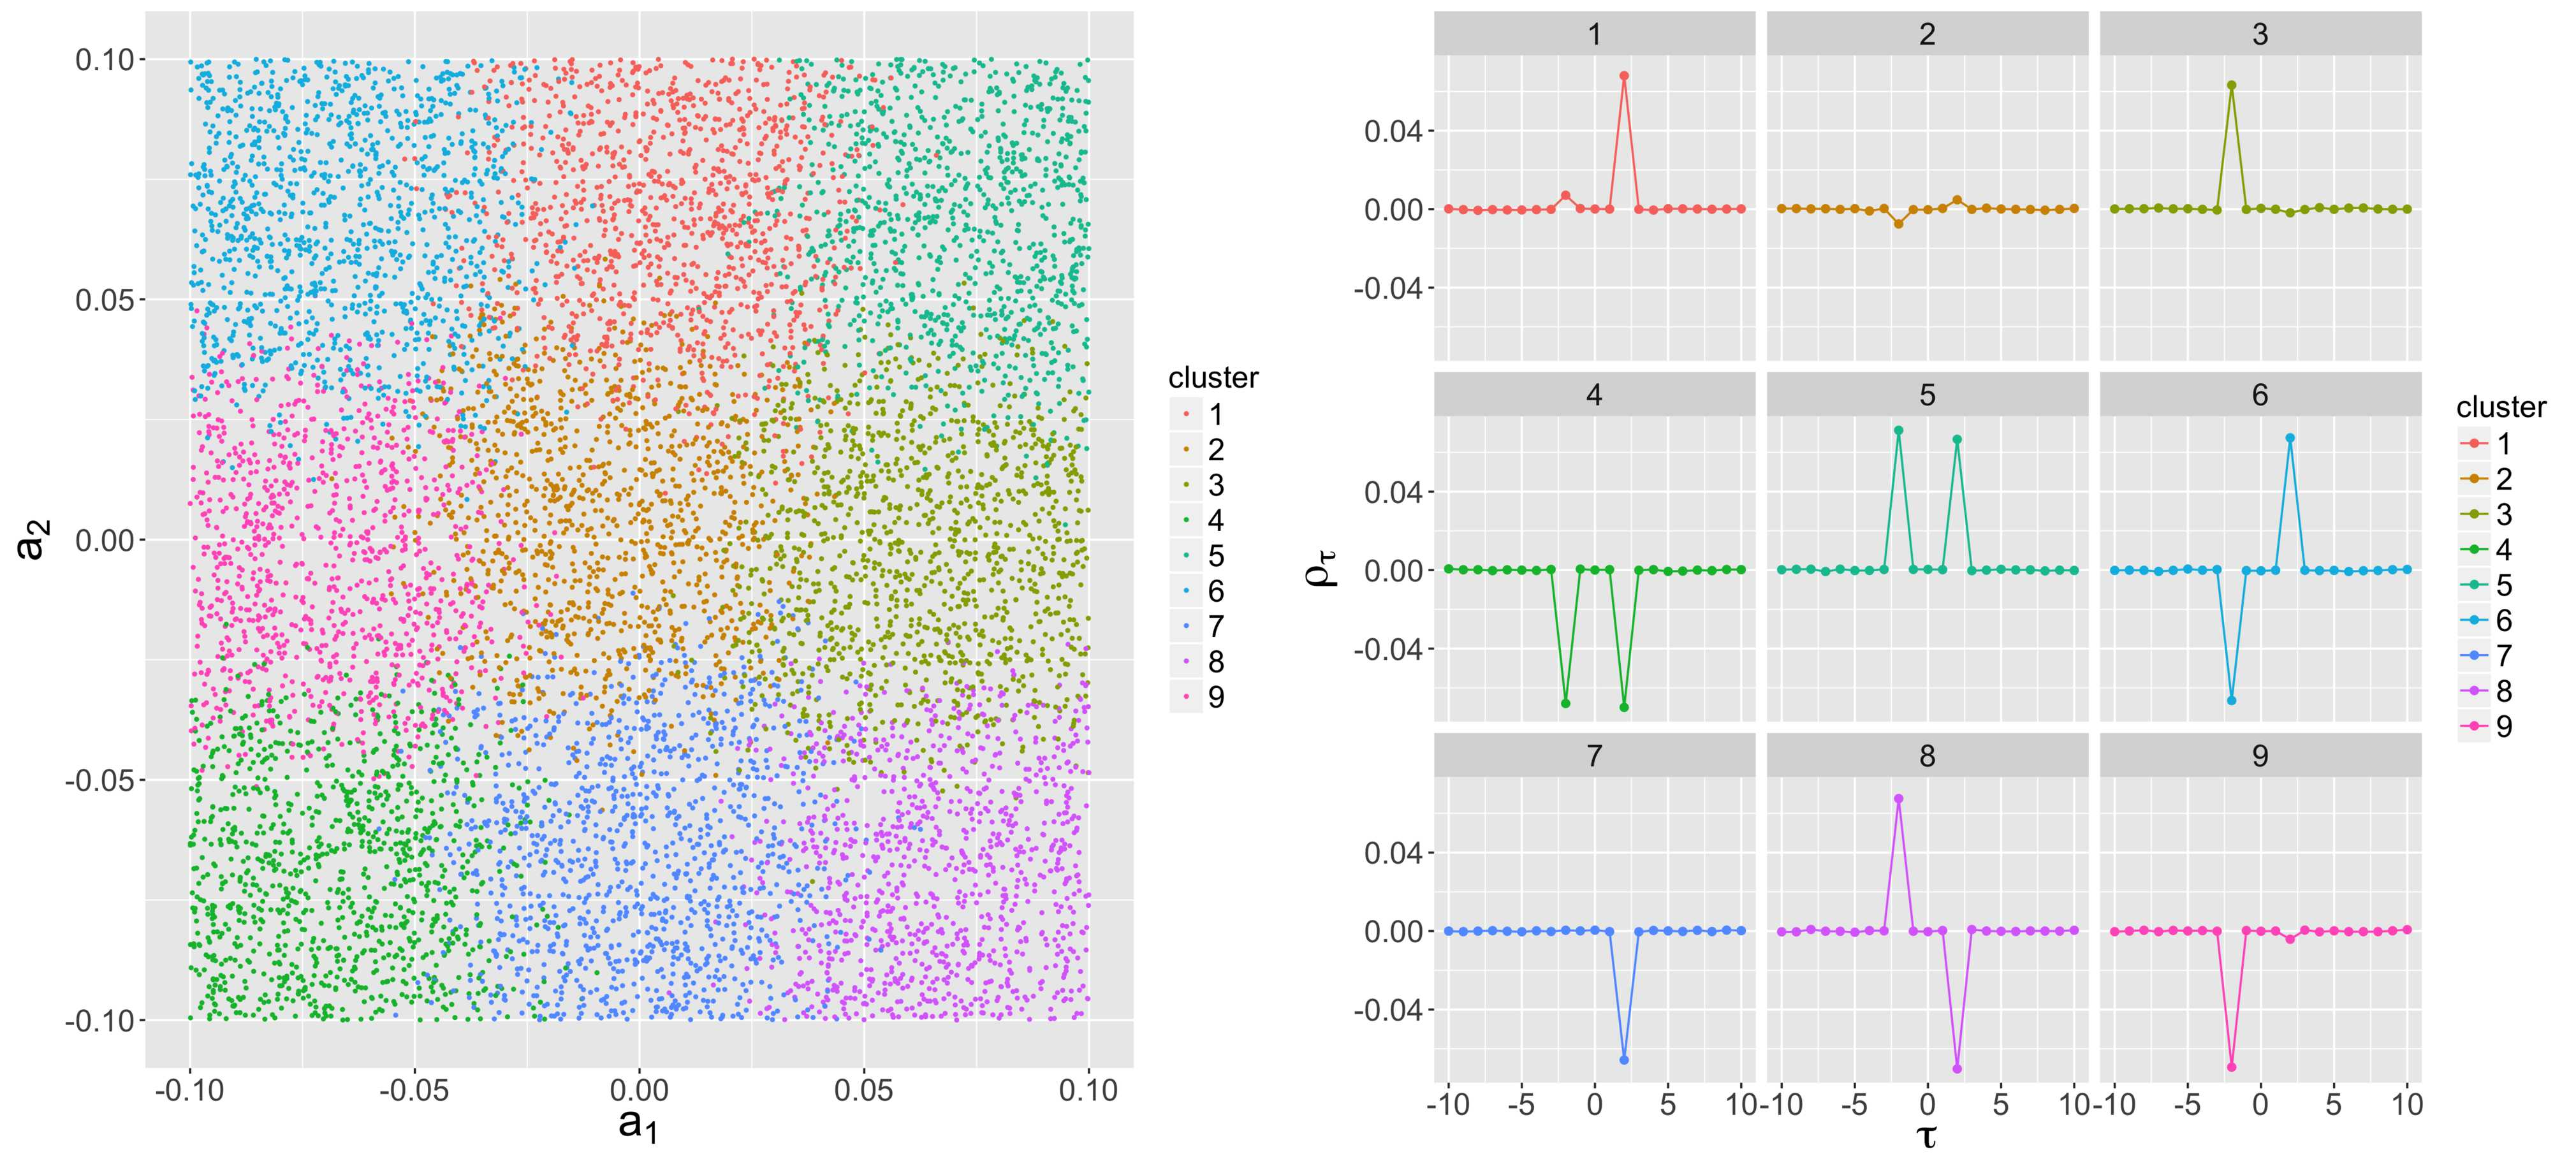
\includegraphics[width=\linewidth]{Figures/Final/4-2-2-fig-causalityregimes-arma.jpg}
	\caption[Auto-regressive time-series][Séries temporelles auto-régressives]{\textbf{Estimation of correlation regimes of auto-regressive time series.}\label{fig:causalityregimes:arma}}{\textbf{Estimation des régimes de corrélation dans le cas de séries temporelles auto-régressives linéaires.} Résultats de la méthode de classification des régimes pour des processus AR simples. Nous simulons $b = 10000$ séries temporelles de longueur $t_f = 10000$, avec des coefficients aléatoires $(a_1,a_2) \in [-0.1,0.1]$ et un délai $\tau_0 = 2$. (\textit{Gauche}) Valeur des coefficients $(a_1,a_2)$, la couleur donnant le cluster obtenu ; (\textit{(Droite)}) Trajectoires de centroïdes correspondants. Nous retrouvons les profils stylisés attendus, qui correspondent aux valeurs relatives des paramètres : par exemple, le cluster 1 est pour $a_1$ faible et $a_2$ fort, et correspond bien à une situation où $\rho_+$ existe c'est-à-dire une configuration $X\rightarrow Y$, et le signe de $\rho_+$ correspond à $a_2 >0$. \label{fig:causalityregimes:arma}}
\end{figure}
%%%%%%%%%%%%%



\subsubsection{Urban growth model}{Modèle de croissance urbaine}

\bpar{
This method must first be tested and partially validated, what we propose to do on synthetic data, what allows a more refined knowledge of the behavior of models~\cite{raimbaulthalshs01514415}. Echoing the example of relations between transportation networks and territories that introduced the research question before, we generate stylized urban configurations in which network and density mutually interact, and for which causalities are not obvious \emph{a priori} knowing the parameters of the generative model.
}{
Cette méthode doit être testée et validée sur un système plus proche de nos préoccupations, ce que nous faisons à nouveau sur des données synthétiques.  En écho à l'exemple des relations entre réseaux de transport et territoires qui a permis d'introduire notre problématique précédemment, nous proposons de générer des configurations urbaines stylisées dans lesquelles réseau et densité s'influencent mutuellement, et pour lesquelles les causalités ne sont pas évidentes \emph{a priori} étant donné les paramètres du modèle génératif.
}
% méthode qui permet une connaissance plus fine des comportements des modèles \cite{raimbault2016generation}.


\bpar{
\cite{raimbault2014hybrid} describes and explores a simple model of urban morphogenesis (the RBD model) that fits perfectly these constraints. Indeed, explicative variables of urban growth, processes of network extension and the coupling between urban density and the network are relatively simple. However, except for extreme cases (for example when distance to the center solely determines land value, the network will depend on density in a causal way; when only the distance to the network counts, the causality will be inverted), mixed regimes do not exhibit obvious causalities. It is for this reason an ideal case to test if the method is able to detect some.
}{
\cite{raimbault2014hybrid} décrivent et explorent un modèle simple de morphogenèse urbaine\footnote{Nous n'explorons pas ici le concept de morphogenèse, qui fera l'objet du chapitre~\ref{ch:morphogenesis}, mais utilisons ce modèle comme producteur de données synthétiques.} (modèle RBD) répondant à ces contraintes. Ce modèle est décrit en détails pour la configuration dans laquelle nous l'utilisons en Encadré~\ref{frame:causalityregimes:rbd}. Les variables explicatives de la croissance urbaine, les processus d'extension du réseau et le couplage entre densité urbaine et réseau ne sont pas trop complexes. Cependant, hormis dans des cas particuliers (par exemple lorsque la distance au centre détermine la valeur foncière uniquement, le réseau dépendra de manière causale de la densité, ou lorsque la distance au réseau seule compte, la causalité sera inversée), les régimes mixtes ne présentent pas de causalités évidentes : c'est donc un cas adapté pour tester si la méthode est capable d'en détecter. Les données synthétiques nous permettent de contrôler la cohérence dans les cas où la relation est attendue.
}


%%%%%%%%%%%%%
\begin{figure}[h!]
\begin{mdframed}
Le modèle RBD suppose une grille de côté $N$, dont les cellules ont un état binaire (occupée ou non). Dans la version utilisée, il existe un unique centre urbain (noeud particulier du réseau) et le réseau de transport est initialement nul. Chaque cellule $i$ est caractérisée par les variables $x_d (i)$ (densité de population dans un rayon fixé $r=5$), $x_r (i)$ (distance euclidienne à la route la plus proche) et $x_c (i)$ (distance au centre via le réseau). Ces variables permettent de calculer une valeur de potentiel pour chaque cellule $U_i = \sum w_k \tilde{x}_k (i)$, où les $w_k$ sont des paramètres du modèle permettant d'influencer les formes urbaines produites et $\tilde{x}_k(i)$ les variables normalisées sur l'ensemble des cellules par $\tilde{x}_k(i) = \frac{\max_i x_k (i) - x_k (i)}{\max_i x_k (i) - \min_i x_k (i)}$.

Le potentiel peut être interprété comme une utilité agrégeant les préférences des agents devant se localiser. Une répulsion à la densité donnera par exemple des formes urbaines très dispersées.

Le modèle évolue séquentiellement en peuplant progressivement la grille. À chaque pas de temps :
\begin{itemize}
	\item les $N_G$ cellules avec plus grande valeur $U_i$ sont occupées de manière simultanée ;
	\item si une cellule nouvellement peuplée est à une distance au réseau supérieure à un seuil $\theta_d$ (que nous fixerons ici à $\theta_d = 5$), celle-ci est connectée au réseau par une nouvelle route prenant le chemin le plus court.
\end{itemize}

La croissance s'arrête à un temps final fixé $t_f$.

\medskip

% here example de configs
%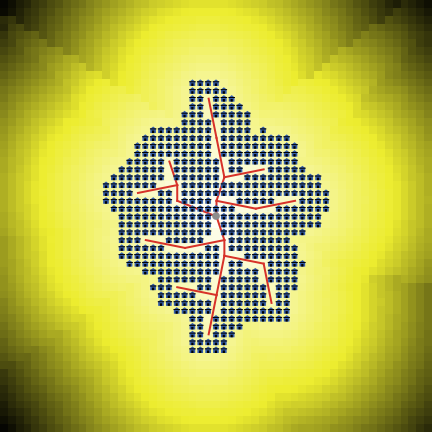
\includegraphics[width=0.32\linewidth]{Figures/CausalityRegimes/ex_60_wdens0_wroad1_wcenter1_seed272727}
%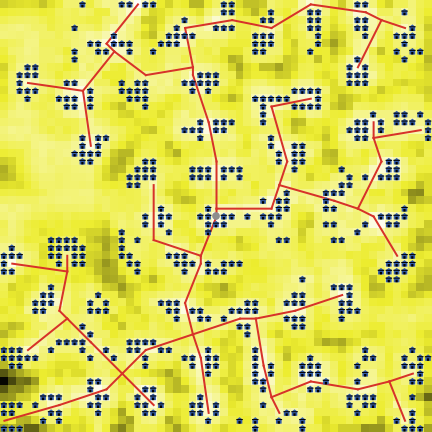
\includegraphics[width=0.32\linewidth]{Figures/CausalityRegimes/ex_60_wdens1_wroad1_wcenter0_seed272727}
%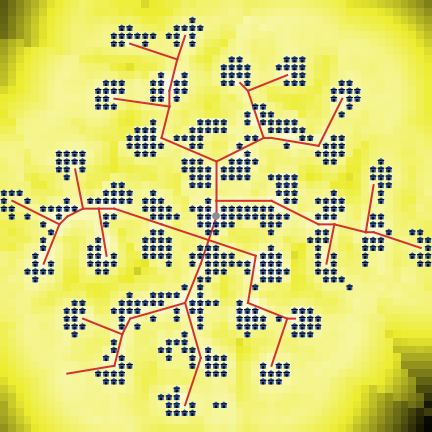
\includegraphics[width=0.32\linewidth]{Figures/CausalityRegimes/ex_60_wdens1_wroad1_wcenter1_seed272727}
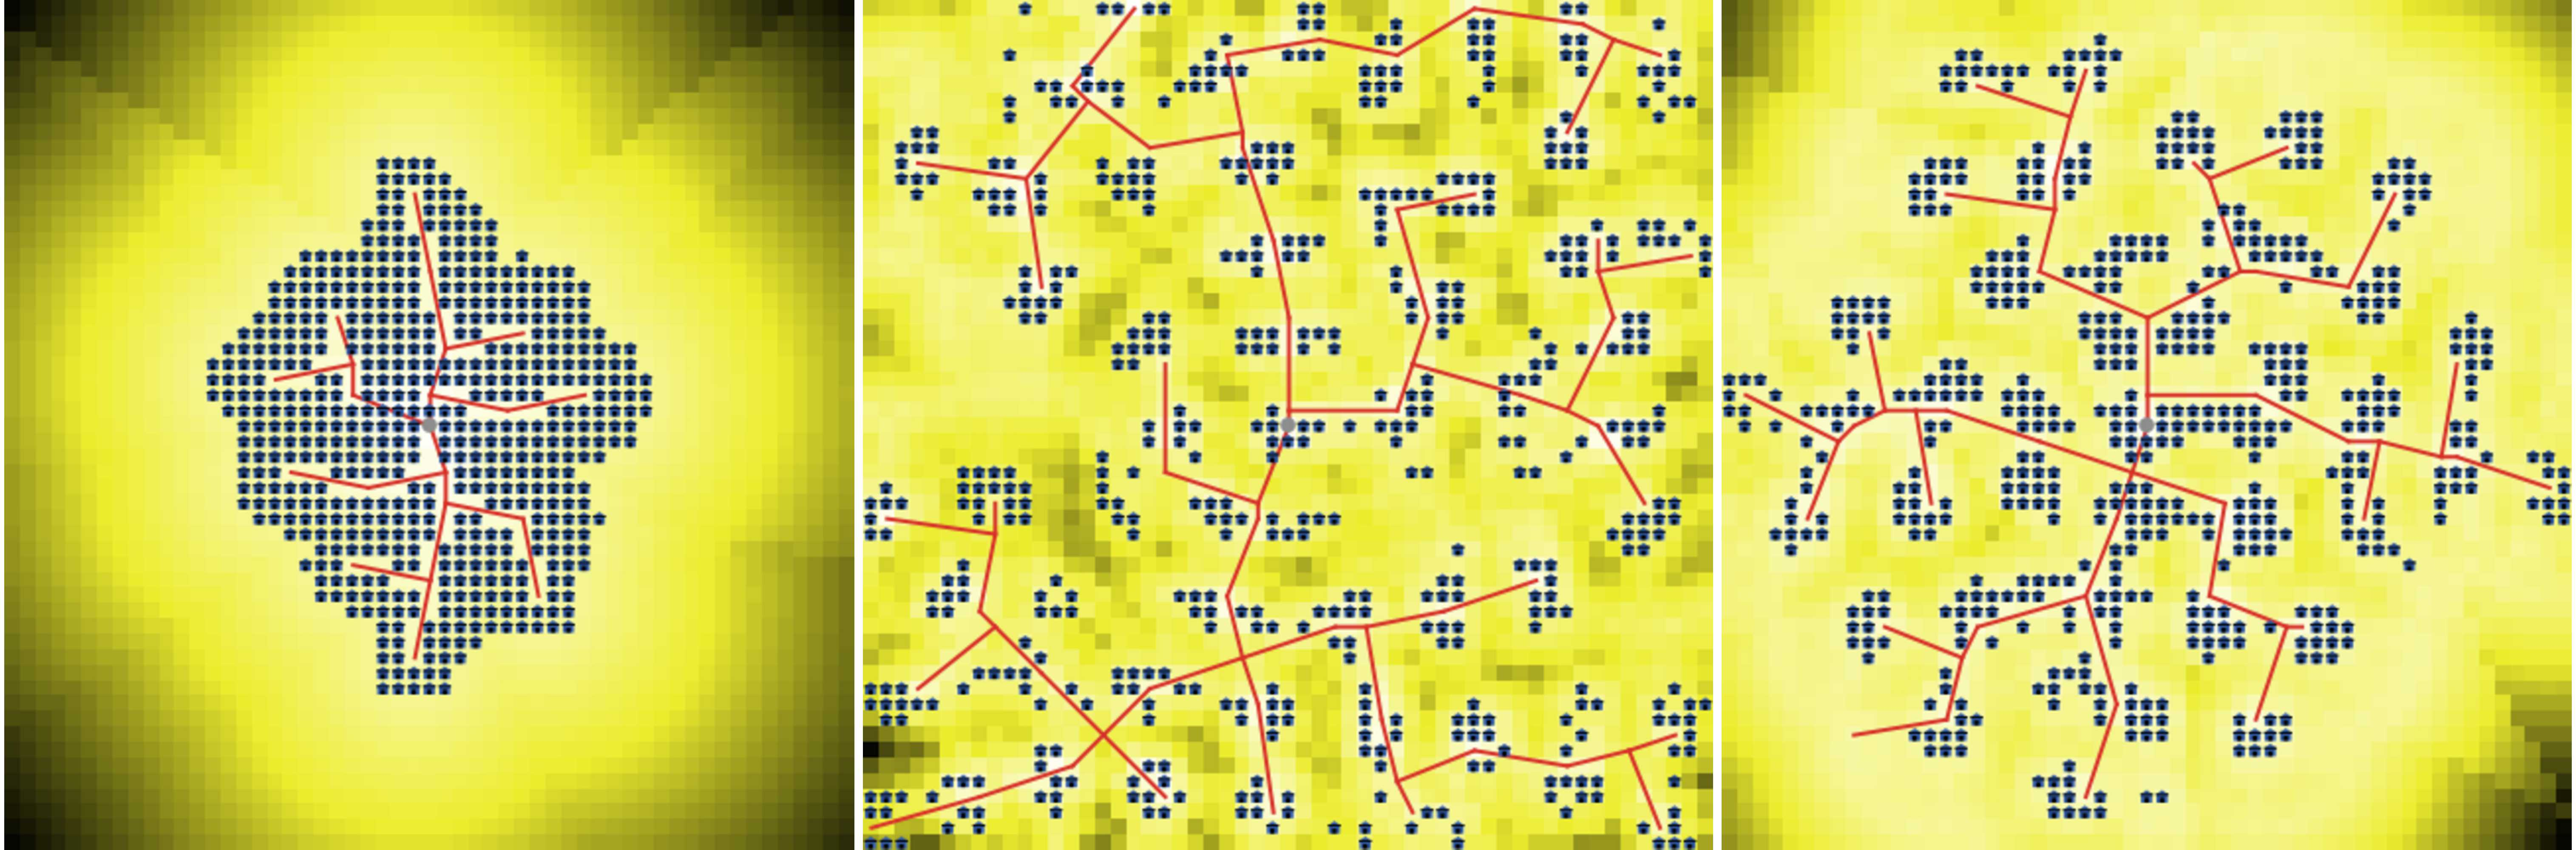
\includegraphics[width=\linewidth]{Figures/Final/4-2-2-frame-causalityregimes-rdb.jpg}
\textit{Exemples de configurations finales variées, obtenues avec les paramètres de poids $(w_{d},w_{c},w_{r})$ valant respectivement $(0,1,1)$,$(1,0,1)$, et $(1,1,1)$.}

\medskip

\framecaption{\textbf{Description of the RBD model.}\label{frame:causalityregimes:rbd}}{\textbf{Description du modèle RBD.}\label{frame:causalityregimes:rbd}}
\end{mdframed}
\end{figure}
%%%%%%%%%%%%%





\bpar{
 We use an applied implementation\footnote{available on the open repository of the project at \\\texttt{https://github.com/JusteRaimbault/CityNetwork/tree/master/Models/Simple/ModelCA}} of the original model, allowing to capture the values of studied variables for each cell of the cellular automaton and for each time step, and to calculate the lagged correlations in the sense described before, between variables of the model. We explore a grid of the parameter space of the RBD model, making the weight parameters for density, distance to center and distance toi network vary\footnote{The model works the following way: a value of cells is determined by the weighted average of these different explicative variables, value that determines the growth of new patches at the next time step.}, that we write respectively $(w_{d},w_{c},w_{r})$, in $\left[0;1\right]$ with a step of $0.1$. Other parameters are fixed to their default values given by~\cite{raimbault2014hybrid}. For each parameter value, we proceed to $N=100$ repetitions, what is enough for a good convergence of indicators. Explorations are done with the OpenMole software~\cite{reuillon2013openmole}, the large number of simulations (1,330,000) implying the use of a computation grid.
}{
Nous utilisons une implémentation adaptée\footnote{Le modèle est disponible sur le dépôt ouvert du projet à \url{https://github.com/JusteRaimbault/CityNetwork/tree/master/Models/Simple/ModelCA}.} du modèle initial, permettant de capturer les valeurs des variables étudiées pour chaque cellule et à chaque pas de temps et de calculer les correlations retardées entre variables au sein du modèle. Nous explorons une grille de l'espace des paramètres du modèle RBD, faisant varier les paramètres de poids de la densité $w_d$, de la distance au centre $w_c$ et de la distance au réseau $w_r$ (voir Encadré~\ref{frame:causalityregimes:rbd} de description du modèle), dans $\left[0;1\right]$ avec un pas de $0.1$. Les autres paramètres sont fixés à leur valeurs par défaut données par \cite{raimbault2014hybrid}. Pour chaque valeur des paramètres, nous procédons à $N=100$ répétitions ce qui est suffisant pour une bonne convergence des indicateurs. Les explorations sont effectuées via le logiciel OpenMole~\cite{reuillon2013openmole}, le grand nombre de simulations (1330000) nécessitant l'utilisation d'une grille de calcul\footnote{Les résultats de simulation sont disponibles à \url{http://dx.doi.org/10.7910/DVN/KGHZZB}.}.
}



\bpar{
We compute for all patches the lagged correlations with the unbiased Pearson estimator between the variations of the following variables\footnote{Computing the correlations directly on the variables makes no sense since their value has no absolute meaning.}: local density, distance to center and distance to network.
}{
Nous calculons sur l'ensemble des cellules les corrélations retardées par estimateur de Pearson non biaisé entre les variations des variables suivantes\footnote{Calculer les corrélations sur les variables directement n'a pas de sens puisque leur valeur n'en a pas en absolu.} : densité locale, distance au centre et distance au réseau. Il s'agit des variables explicatives pour la dynamique du modèle, et donc celles sur lesquelles on peut identifier des relations dynamiques entre caractéristiques territoriales locales.
}



%%%%%%%%%%%%%%%
\begin{figure}
\vspace{-0.5cm}
%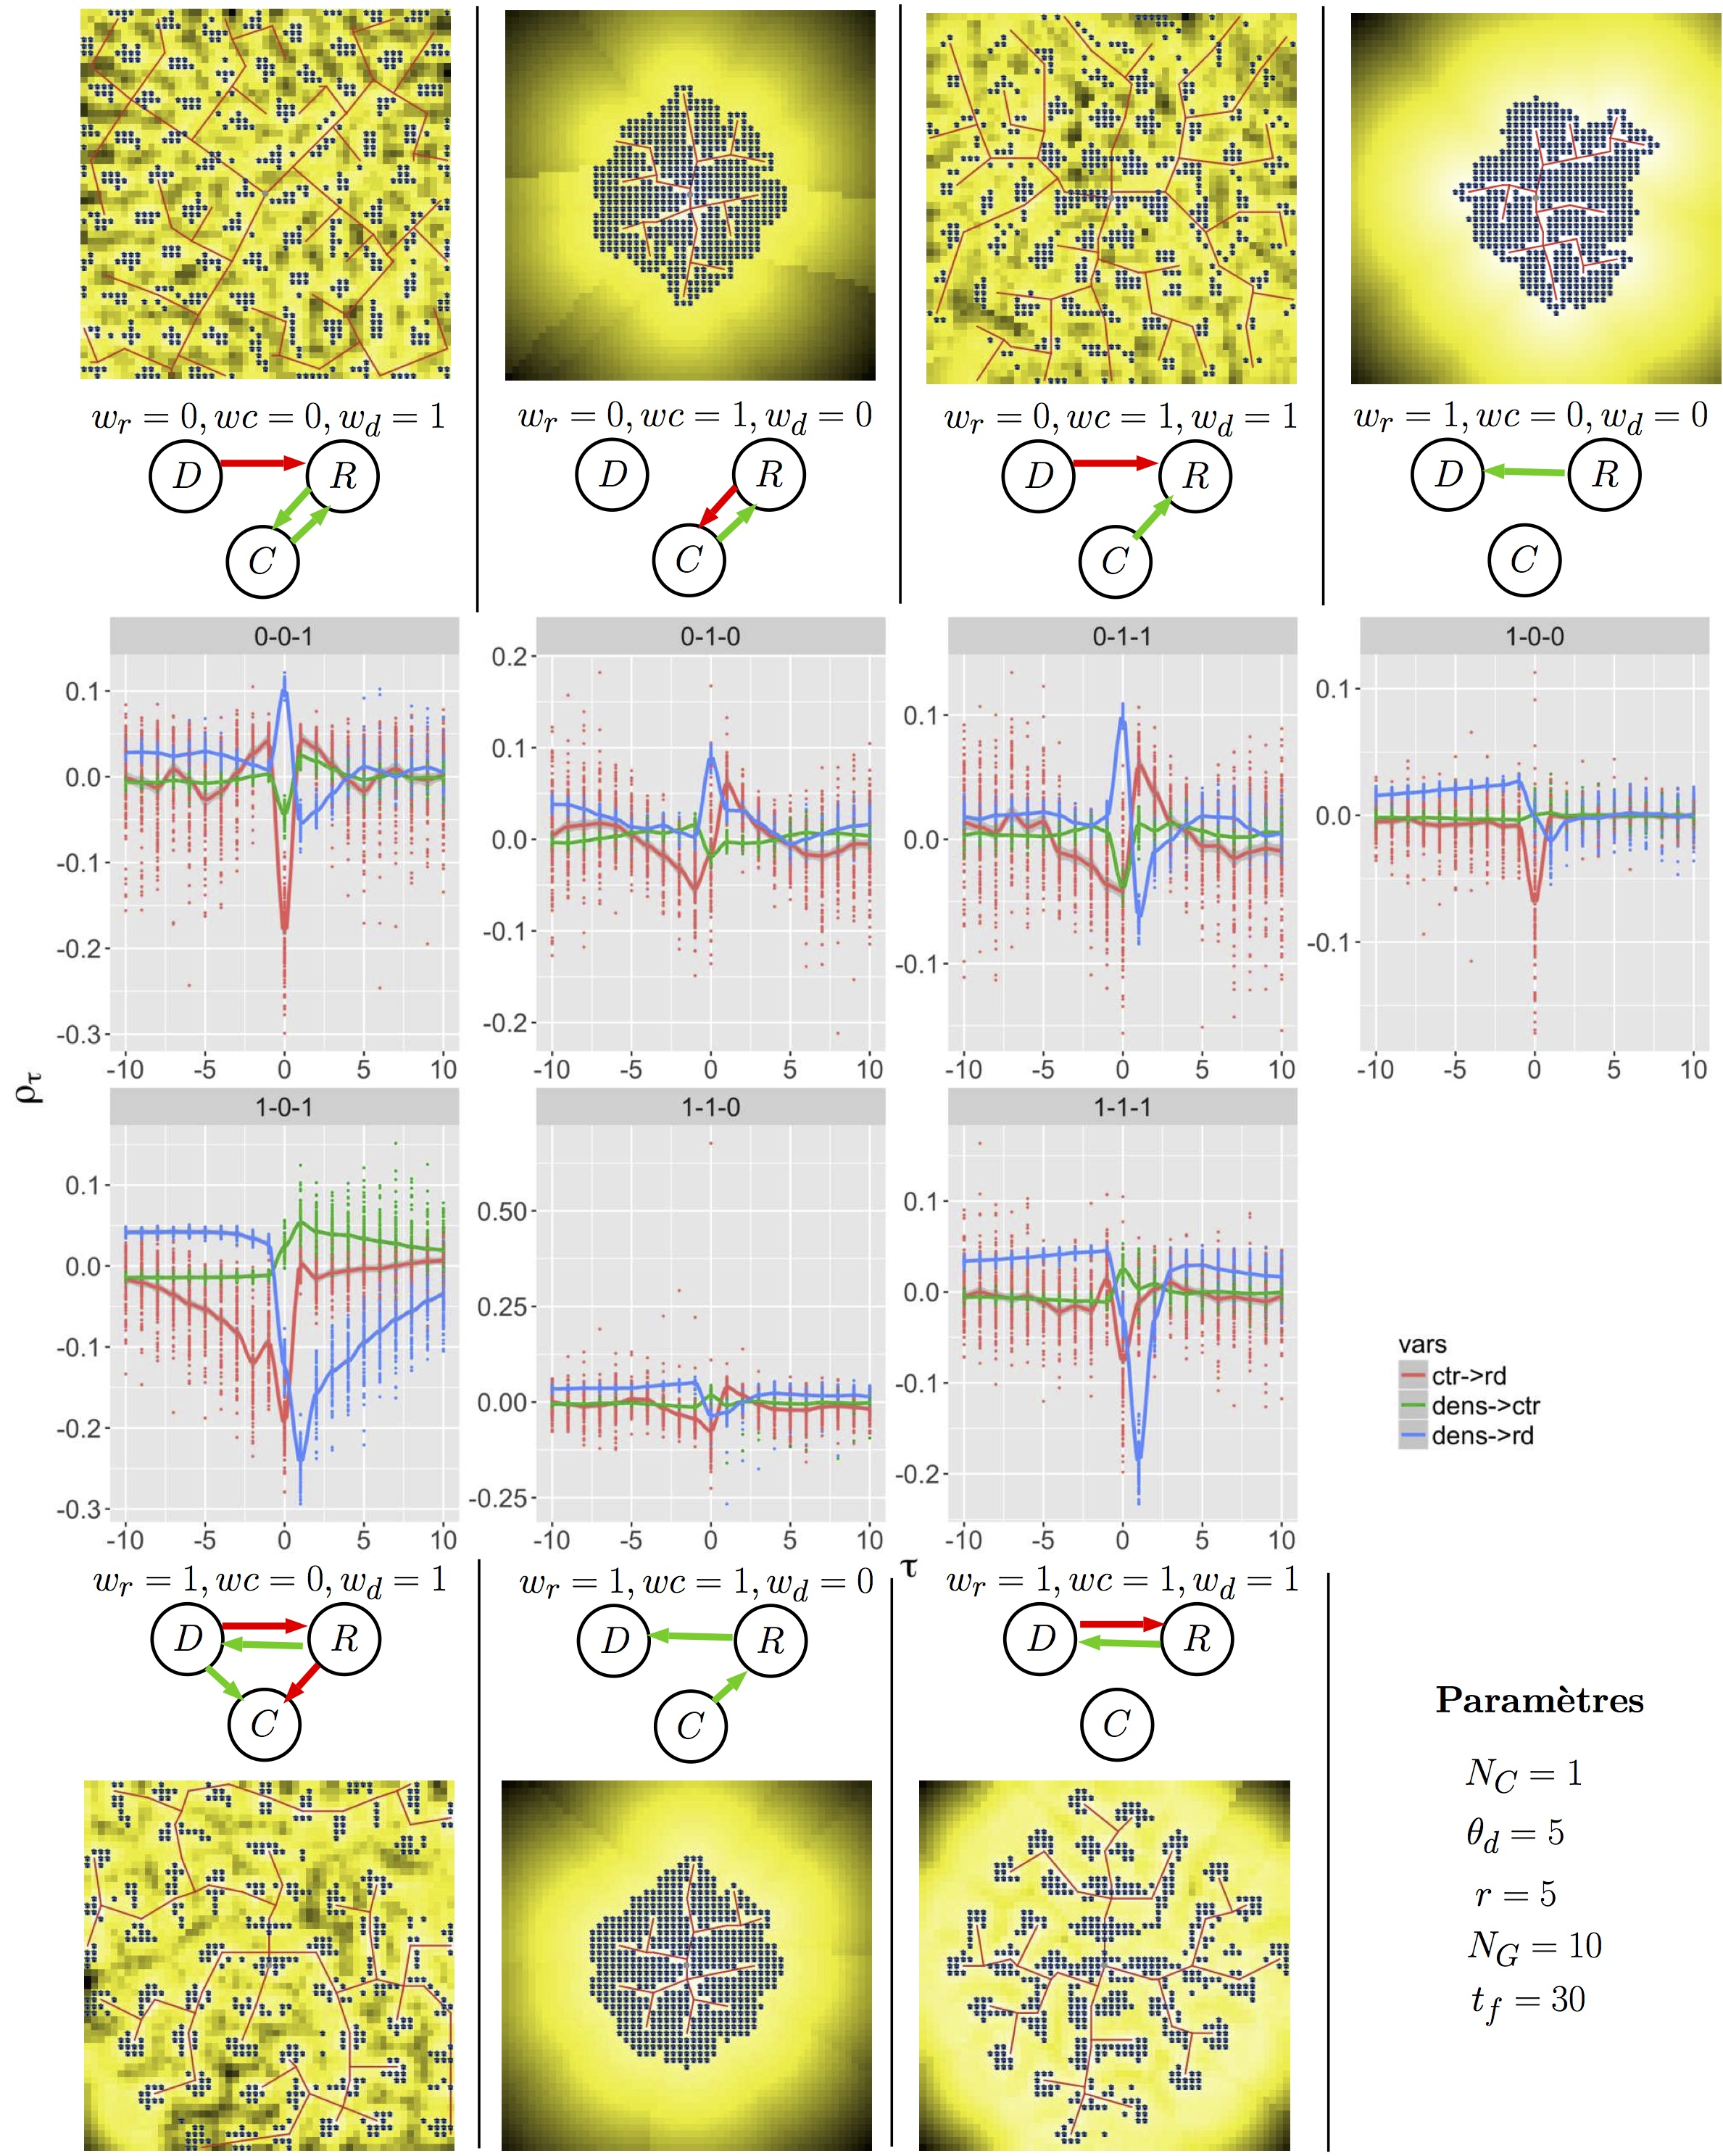
\includegraphics[width=\linewidth]{Figures/CausalityRegimes/synth_extreme.jpg}
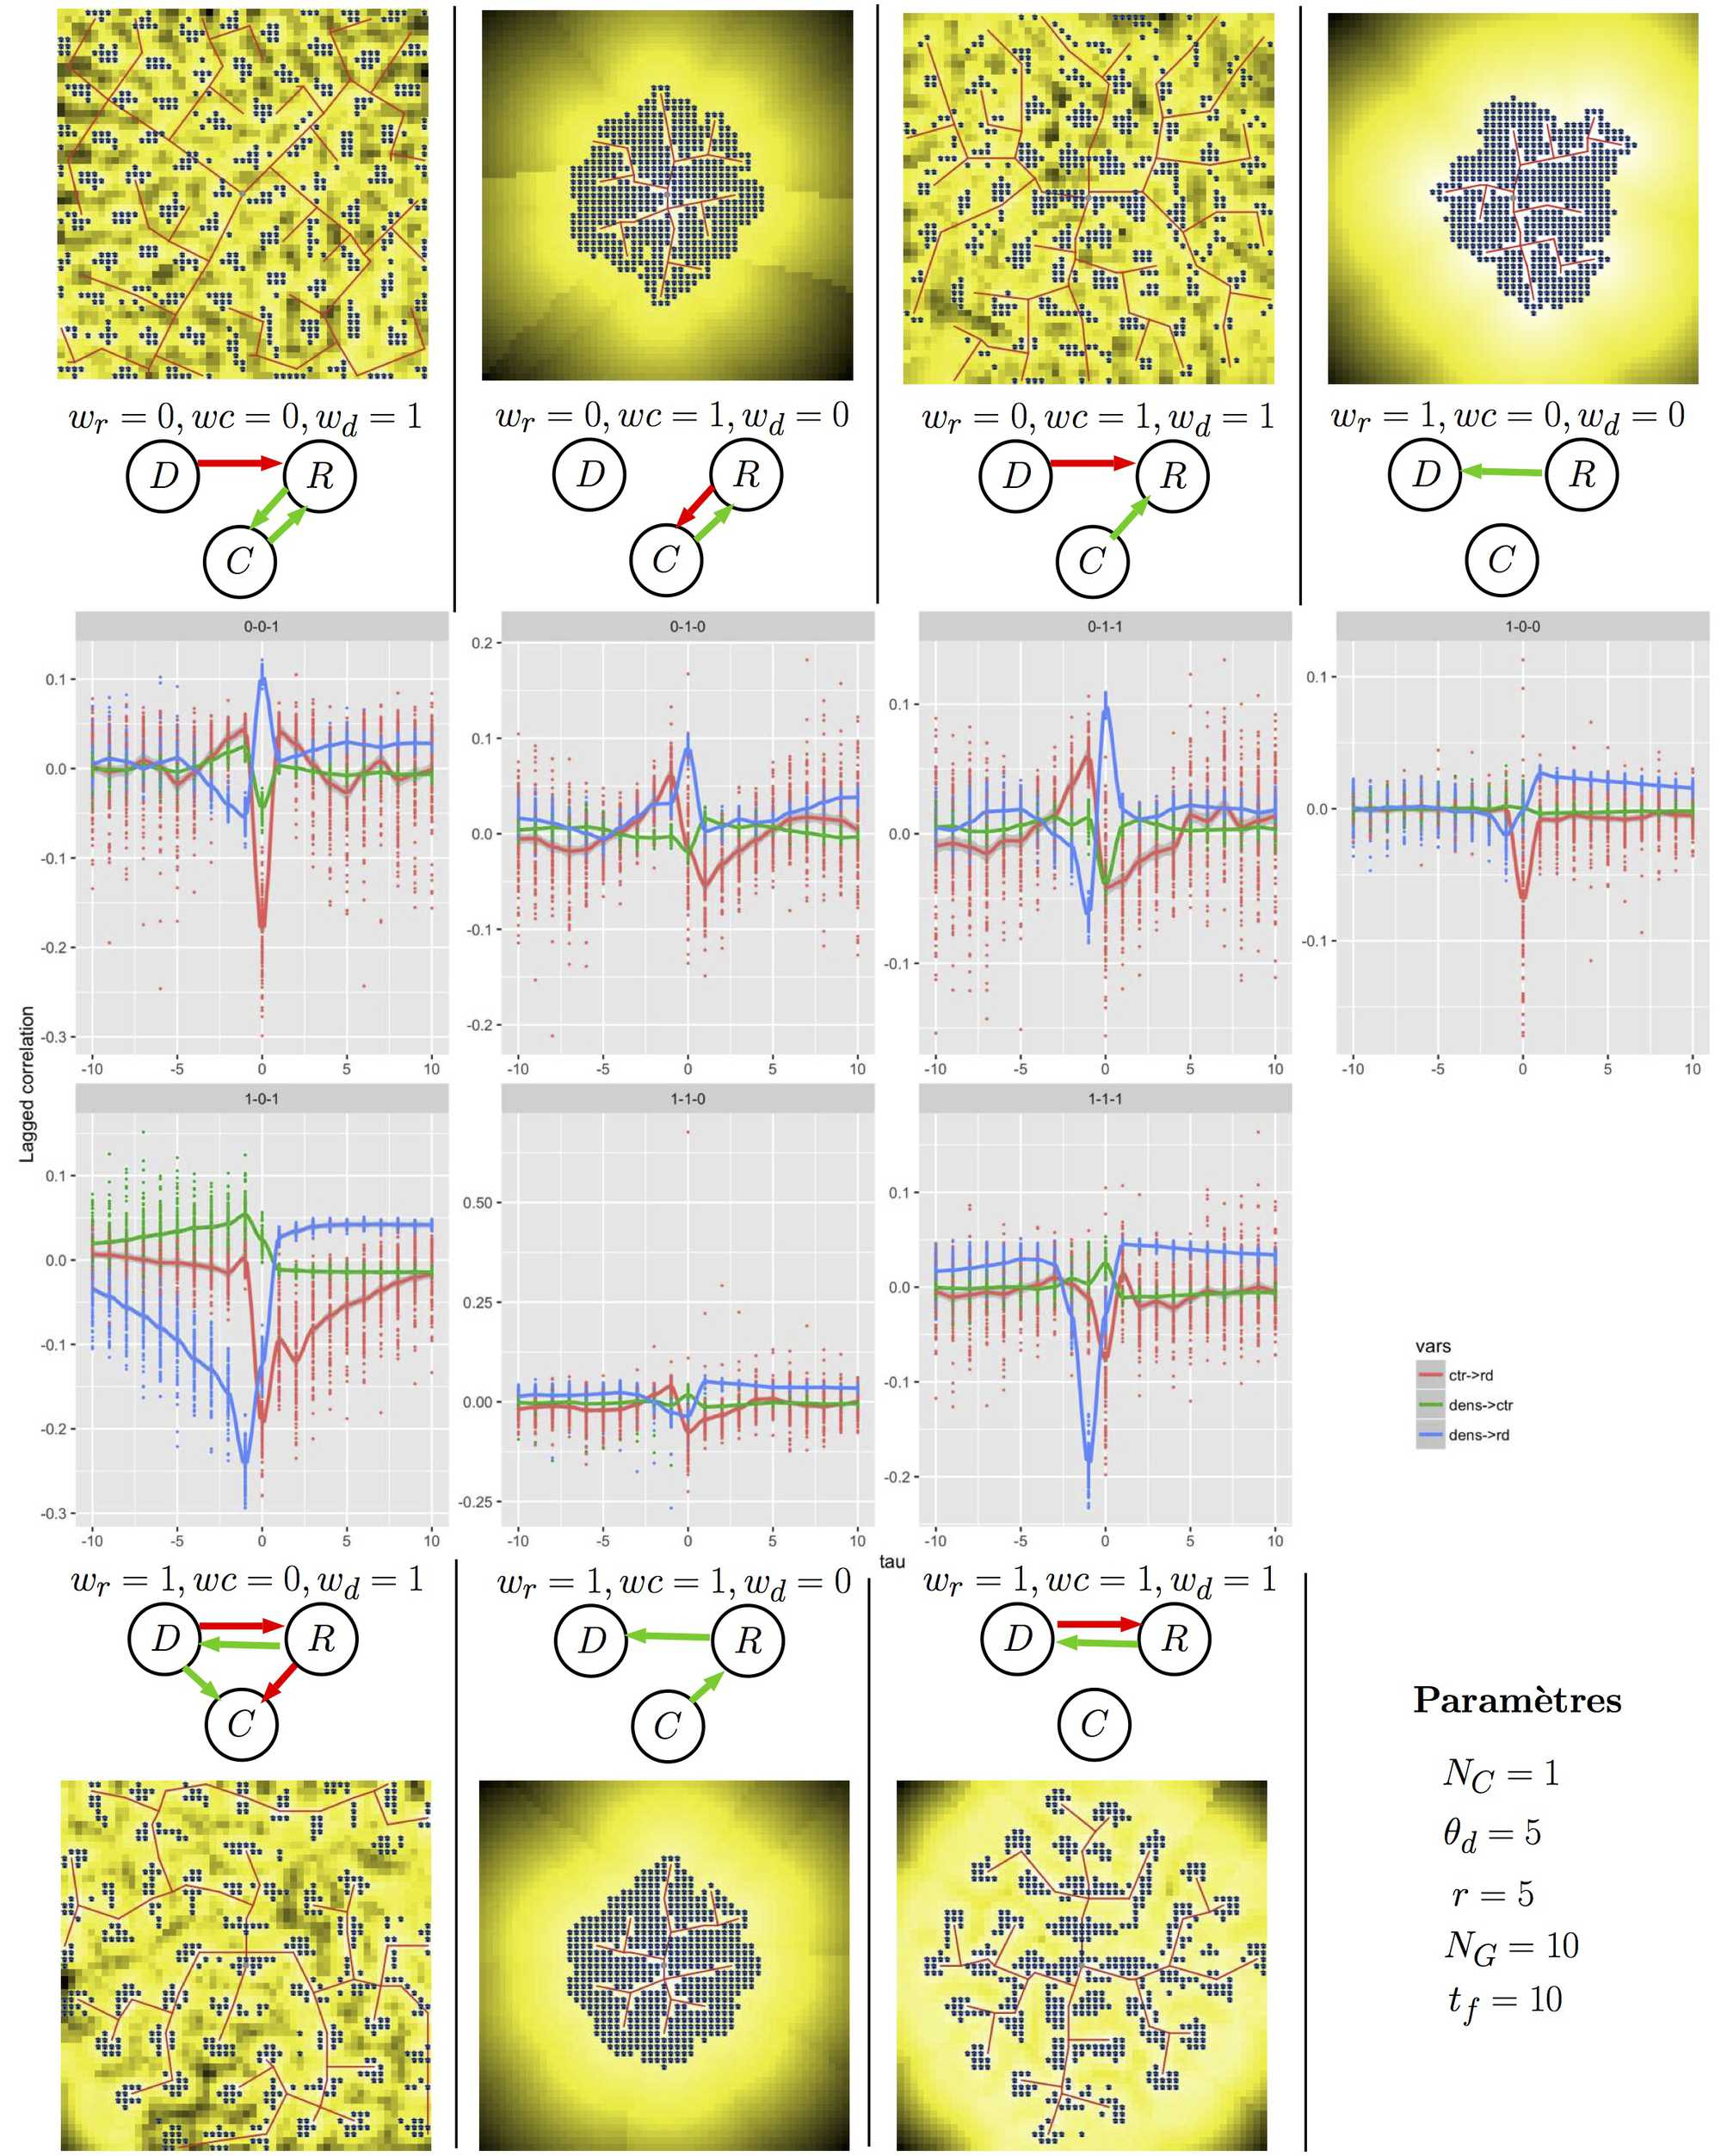
\includegraphics[width=\linewidth,height=0.9\textheight]{Figures/Final/4-2-2-fig-causalityregimes-exrdb.jpg}
\vspace{-0.8cm}
\caption[Correlation in the RBD model][Corrélations dans le modèle RDB]{\textbf{Correlations in the RBD model.} \textbf{(First row)} Example of different final configurations, obtained with $(w_{d},w_{c},w_{r})$ being respectively $(0,1,1)$,$(1,0,1)$, and $(1,1,1)$. \textbf{(Second row)} Lagged correlations, for each combination of parameters in $\{0,1\}$, as a function of the lag $\tau$. The different colors correspond to each couple of variables: distance to the center (\texttt{ctr}, $C$), density (\texttt{dens}, $D$) and distance to the network (\texttt{rd}, $R$). The dots show the extent on all the repetitions of the model (estimators on $i$ and $t$ only).\label{fig:causalityregimes:exrdb}}{\textbf{Correlations retardées dans le modèle RDB.} Corrélations retardées, pour chaque combinaison des valeurs extrêmes pour l'ensemble des paramètres $w_r,w_c,w_d$. Chaque graphe donne la corrélation $\rho_{\tau}$ en fonction du retard $\tau$. Les différentes couleurs correspondent à chaque couple de variables : distance au centre (\texttt{ctr}), densité (\texttt{dens}) et distance au réseau (\texttt{rd}). Les points correspondent aux corrélations individuelles pour chaque répétition du modèle (estimateurs sur $i$ et $t$), tandis que les courbes donnent l'estimateur complet sur l'ensemble des répétitions également. Pour chaque graphe, nous donnons en correspondance directe une configuration finale, et l'interprétation de terme de motifs de causalité sous forme d'un graphe entre les variables. La couleur des liens dirigés donne le signe de la relation (rouge pour corrélation négative, verte pour corrélation positive).\label{fig:causalityregimes:exrdb}}
\end{figure}
%%%%%%%%%%%%%%%



\bpar{
The figure~\ref{fig:exrdb}  shows the behavior of $\rho_{\tau}$ for each couple of variable (undirected, $\tau$ taking negative and positive values), for the combination of extreme values of parameters. We can already see different regimes emerge: for example, $(1,0,1)$ leads to a causality of density on distance to center with a lag $\tau=1$, and a negative causality of density on distance to network with the same lag, whereas distance to the center and to the network are correlated in a synchronous manner.
}{
La Fig.~\ref{fig:causalityregimes:exrdb} montre le comportement de $\rho_{\tau}$ pour chaque couple de variables (non dirigé, $\tau$ prenant des valeurs négatives et positives), pour les combinaisons des valeurs extrêmes des paramètres. Nous donnons également l'interprétation sous forme de graphe de relations entre variables et une illustration de configuration urbaine générée pour les valeurs de paramètres correspondantes.
}

\bpar{}{
Nous voyons un certain nombre de régimes émerger, et pouvons tirer les interprétations synthétiques suivantes :
\begin{itemize}
	\item Le lien négatif $D\rightarrow R$ résulte du mécanisme simple d'extension du réseau : un accroissement de la densité conduit à une diminution de la distance au réseau par la construction d'une nouvelle route. Certaines configurations inhibent ce lien, par l'interaction complexe avec les autres variables (par exemple $(0,1,0)$).
	\item Des graphes de relations élaborés peuvent émerger : $(1,0,1)$ conduit par exemple à une relation circulaire entre distance au réseau et densité, et une causalité de ces deux variables sur la distance au centre.
	\item Des comportements non attendus a priori émergent, comme par exemple la relation circulaire entre distance au réseau et distance au centre pour $(0,0,1)$ où seule la densité joue ; au contraire le modèle fait émerger une relation qui correspond au mécanisme microscopique quand $w_r=1$ seulement.
\end{itemize}
}


L'intérêt de la méthode se précise ici, puisqu'elle permet de dégager des motifs de causalité ``macroscopiques'' (c'est-à-dire effectivement mesurables à un niveau statistique), à partir de motifs ``microscopiques'' (par exemple la règle de connection de la route), et de manière non-linéaire. Des liens qu'on pourrait attendre intuitivement comme $D\rightarrow R$ sont dans certains cas inhibés. Cela confirme la pertinence de la distinction entre les deux premiers niveaux de co-évolution, la co-évolution ``processuelle'' (au niveau des entités ou des processus) et la co-évolution statistique au niveau d'une population.



\subsubsection{Causality regimes}{Régimes de causalité}

\bpar{
To study these behaviors in a systematic way, we propose to identify regimes endogenously, by using non-supervised classification. We apply a \emph{k-means} clustering, robust to stochasticity (5000 repetitions), with the following features: for each couple of variables, $\textrm{argmax}_{\tau} \rho_{\tau}$ and $\textrm{argmin}_{\tau} \rho_{\tau}$ if the corresponding value is such that $\frac{\rho_{\tau}-\bar{\rho}_{\tau}}{\left|\bar{\rho}_{\tau}\right|} > \theta$ with $\theta$ threshold parameter, 0 otherwise. The inclusion of supplementary features of values of $\rho_{\tau}$ does not significantly changes the results, these are therefore not taken into account to reduce the dimension. The choice of the number of clusters $k$ is generally a difficult problem in this kind of approach~\cite{hamerly2003learning}. In our case the system exhibit an convenient structure: the curves of inter-cluster variance proportion and its derivative in figure~\ref{fig:clustering}, as a function of $k$ for different values of $\theta$, show a transition for $\theta = 2$, what gives for the corresponding curve a break around $k=6$. A visual screening of clusters in a principal plan confirms the good quality of the classification for these values. A class corresponds then to a \emph{causality regime}, for which we can represent the phase diagram as a function of model parameters, and also cluster centers profiles (computed as the barycenter in the full initial space) in figure~\ref{fig:clustering}.
}{
Nous démontrons à présent qu'il est possible d'établir une typologie endogène des comportements des corrélations retardées. Afin d'étudier ces comportements de manière systématique, nous proposons d'identifier des régimes de manière endogène, en procédant à un apprentissage non-supervisé. Nous appliquons comme précédemment une classification des \emph{k-means}, robuste à la stochasticité (5000 répétitions), avec les points caractéristiques (\emph{features}) suivants : pour chaque couple de variable, $\textrm{argmax}_{\tau} \rho_{\tau}$ et $\textrm{argmin}_{\tau} \rho_{\tau}$ si la valeur correspondante est telle que $\frac{\rho_{\tau}-\bar{\rho}_{\tau}}{\left|\bar{\rho}_{\tau}\right|} > \theta$ avec $\theta$ paramètre de seuil, 0 sinon. L'inclusion des \emph{features} (variables caractéristiques) supplémentaires des valeurs de $\rho_{\tau}$ n'influence pas significativement les résultats, et celles-ci n'ont pas été prises en compte pour réduire la dimension. Le choix du nombre de clusters $k$ est en général épineux dans ce genre de problème~\cite{hamerly2003learning}, mais dans notre cas le système possède une structure qui lève l'ambiguïté : les courbes de la proportion de variance inter-cluster et de sa dérivée (voir  Fig.~\ref{fig:app:causalityregimes:clustering} en Annexe~\ref{app:sec:causalityregimes}), en fonction de $k$ pour différentes valeurs de $\theta$, présentent une transition pour $\theta = 2$, ce qui donne pour cette courbe une rupture à $k=5$. Un examen visuel des clusters dans un plan principal confirme la bonne qualité de la classification pour ces valeurs. Une classe correspond alors à un \emph{régime de causalité}, dont nous pouvons représenter le diagramme de phase en fonction des paramètres du modèle, ainsi que les trajectoires des centres des clusters (calculées comme barycentre dans l'espace complet initial) en Fig.~\ref{fig:causalityregimes:clustering}.
}




%%%%%%%%%%%%%%%
\begin{figure}
%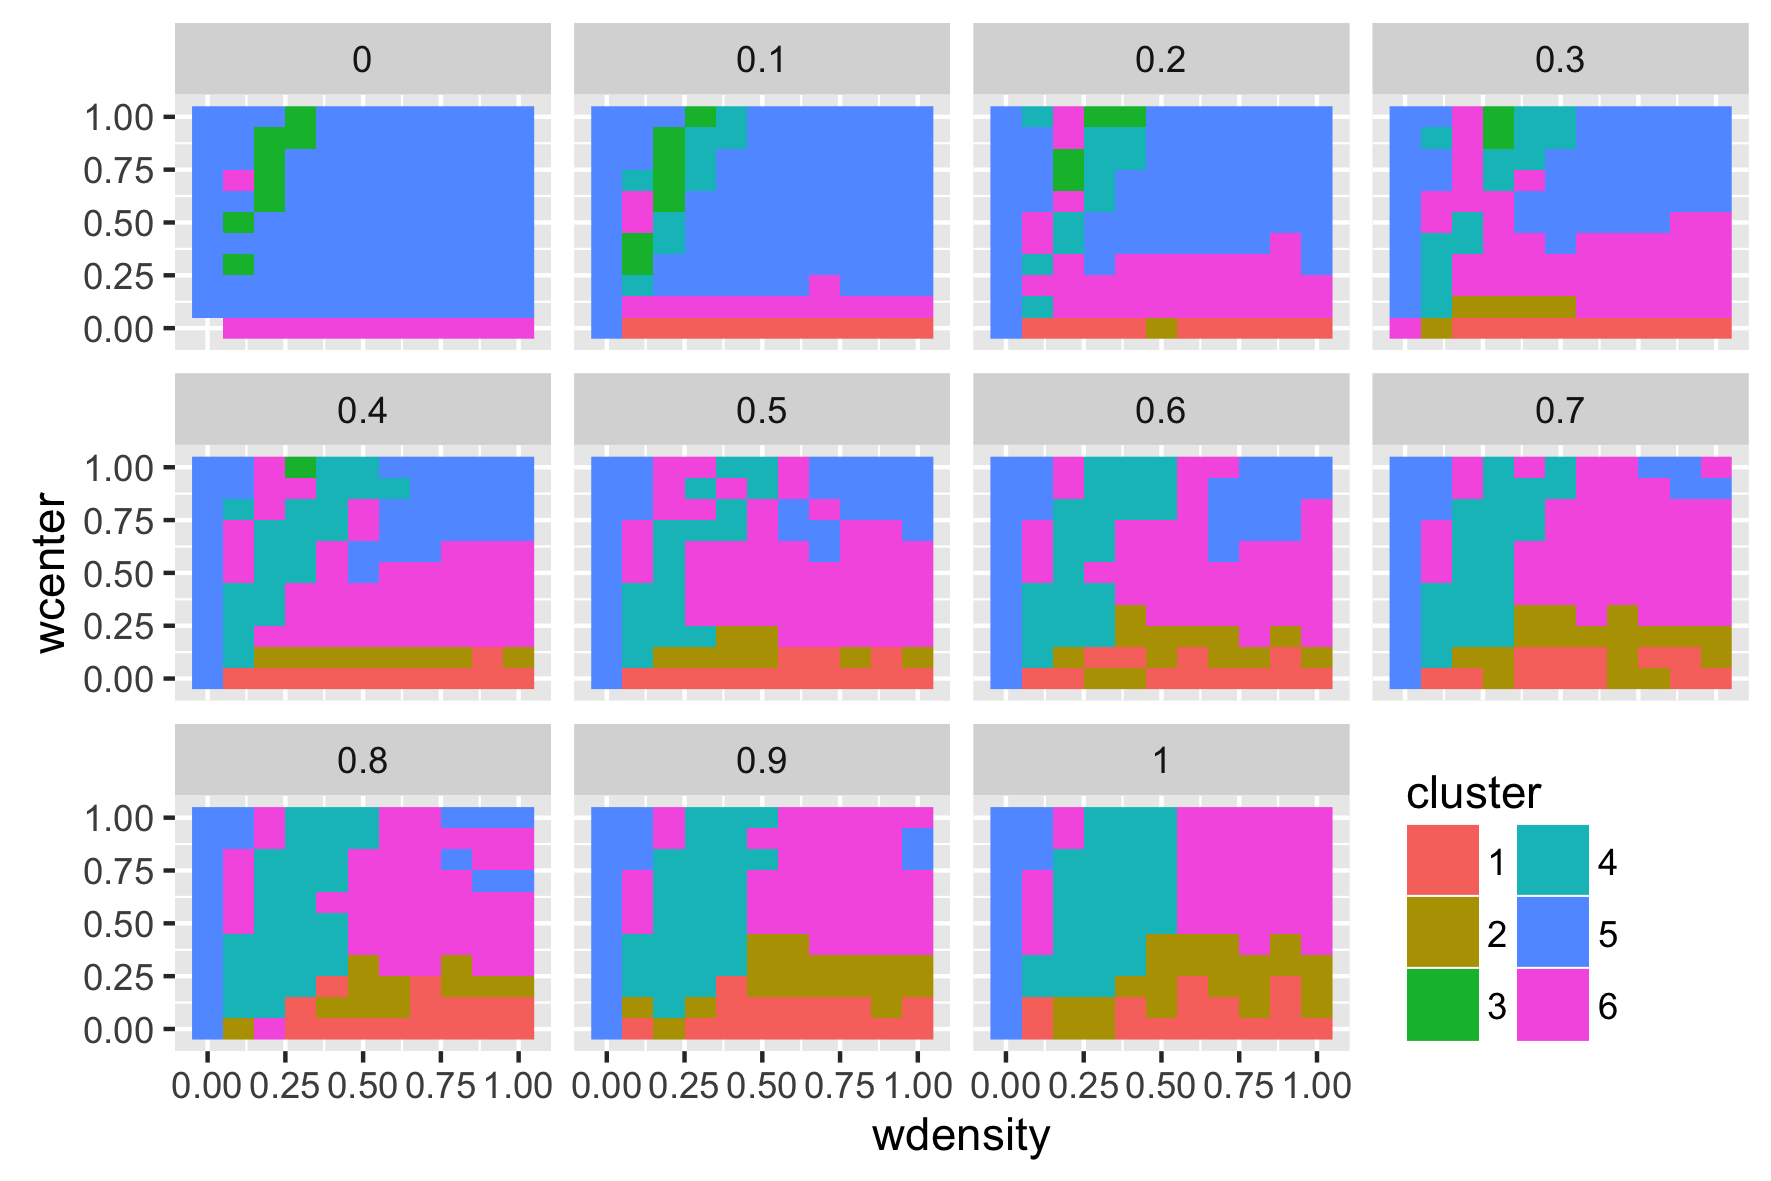
\includegraphics[width=0.59\linewidth]{Figures/CausalityRegimes/clusters-paramfacet_valuesFALSEtheta2_k6}\\
%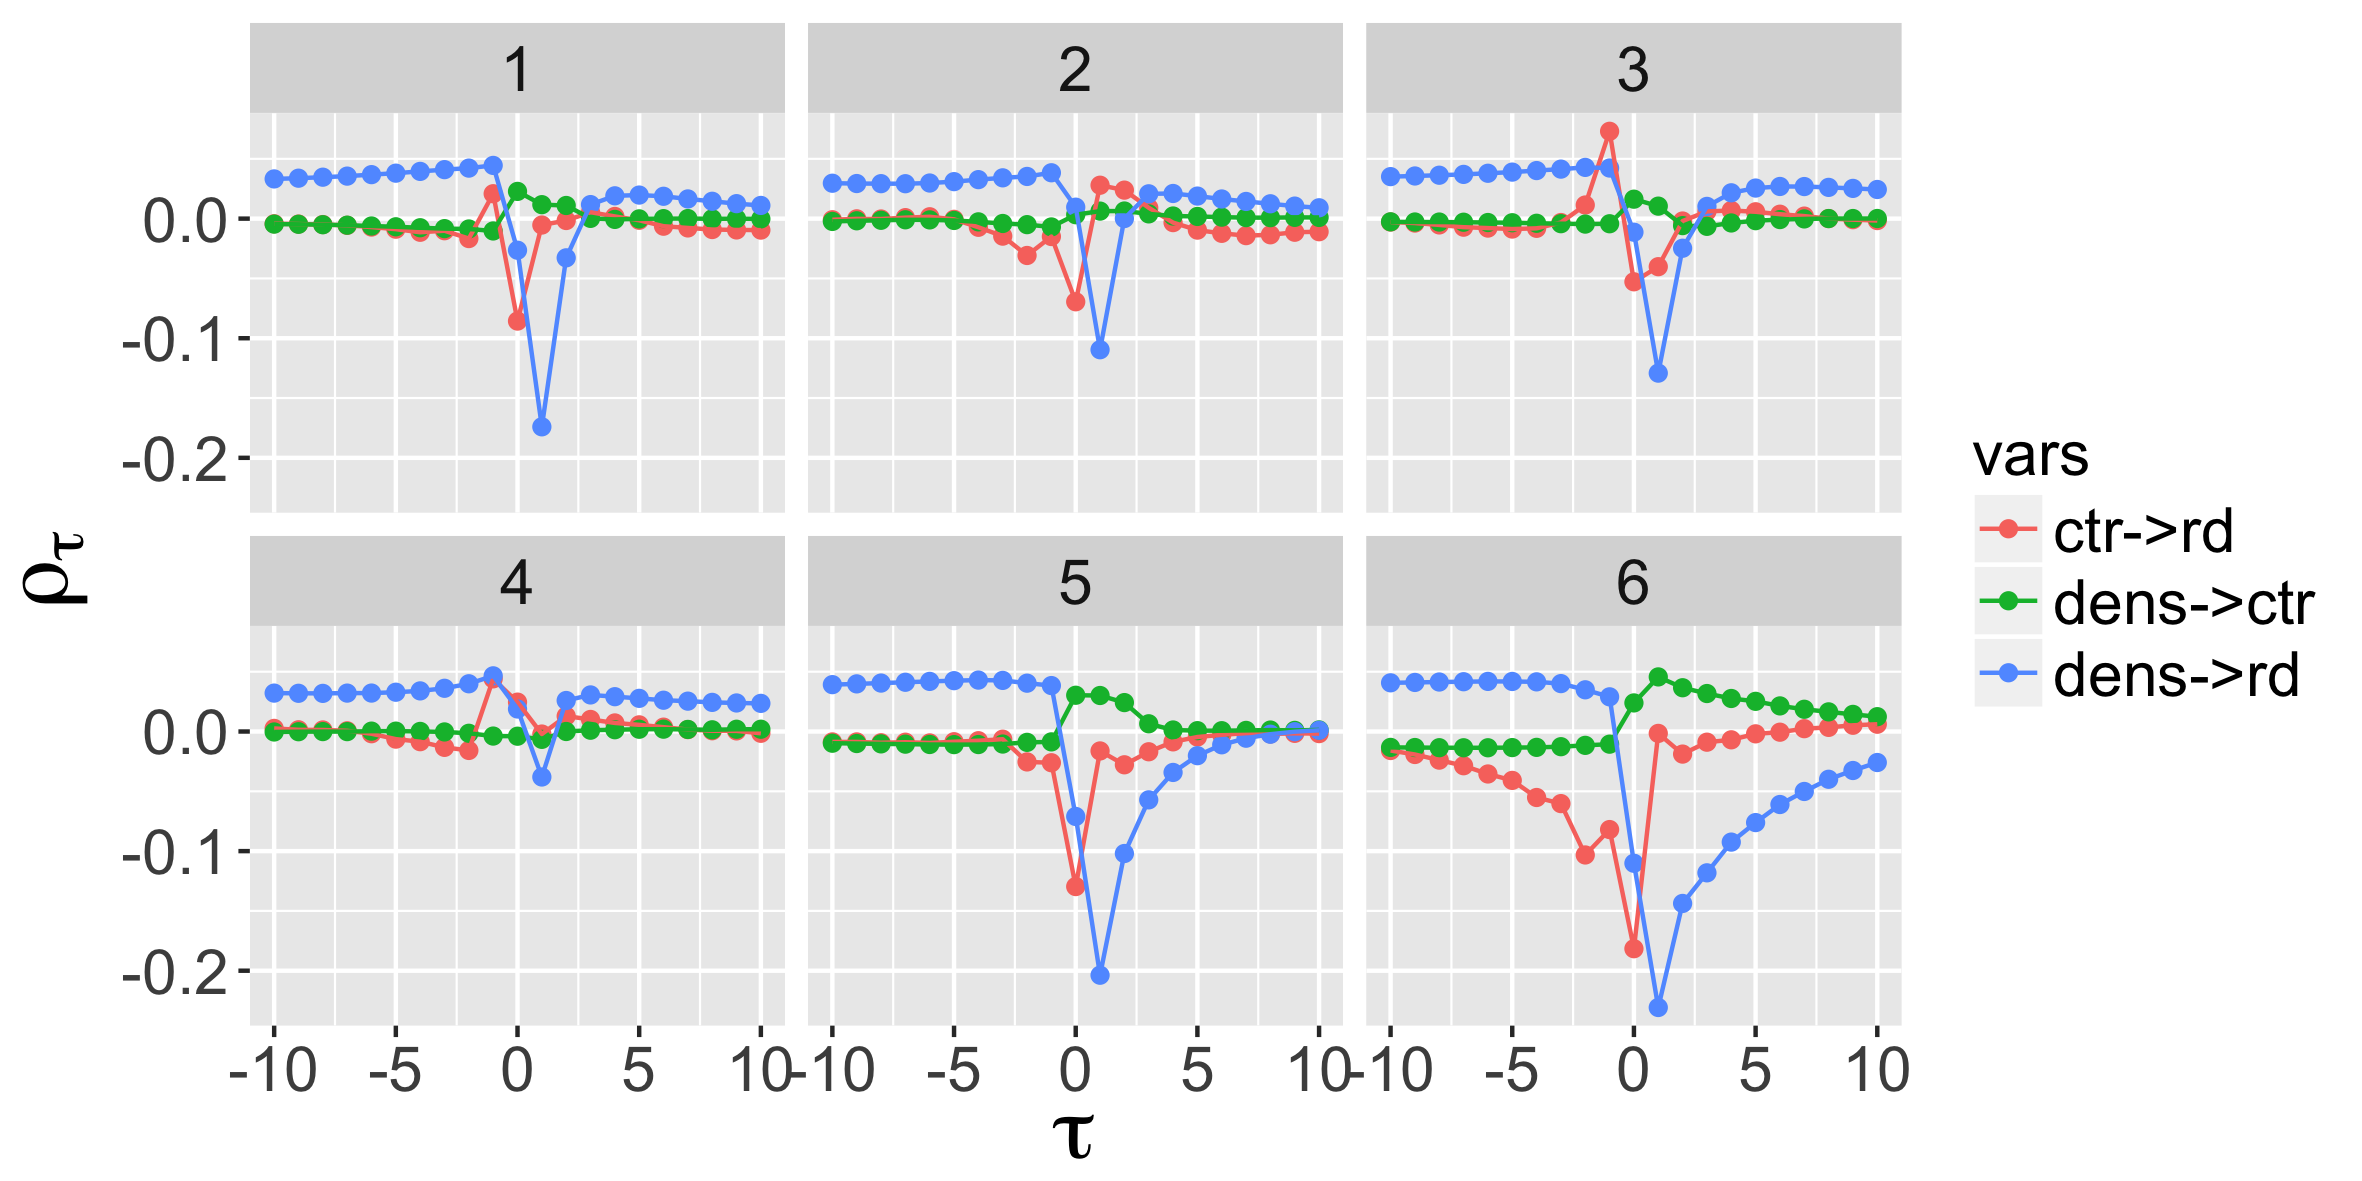
\includegraphics[width=\linewidth]{Figures/CausalityRegimes/clusters-centertrajs-facetclust_valuesFALSEtheta2_k6}]
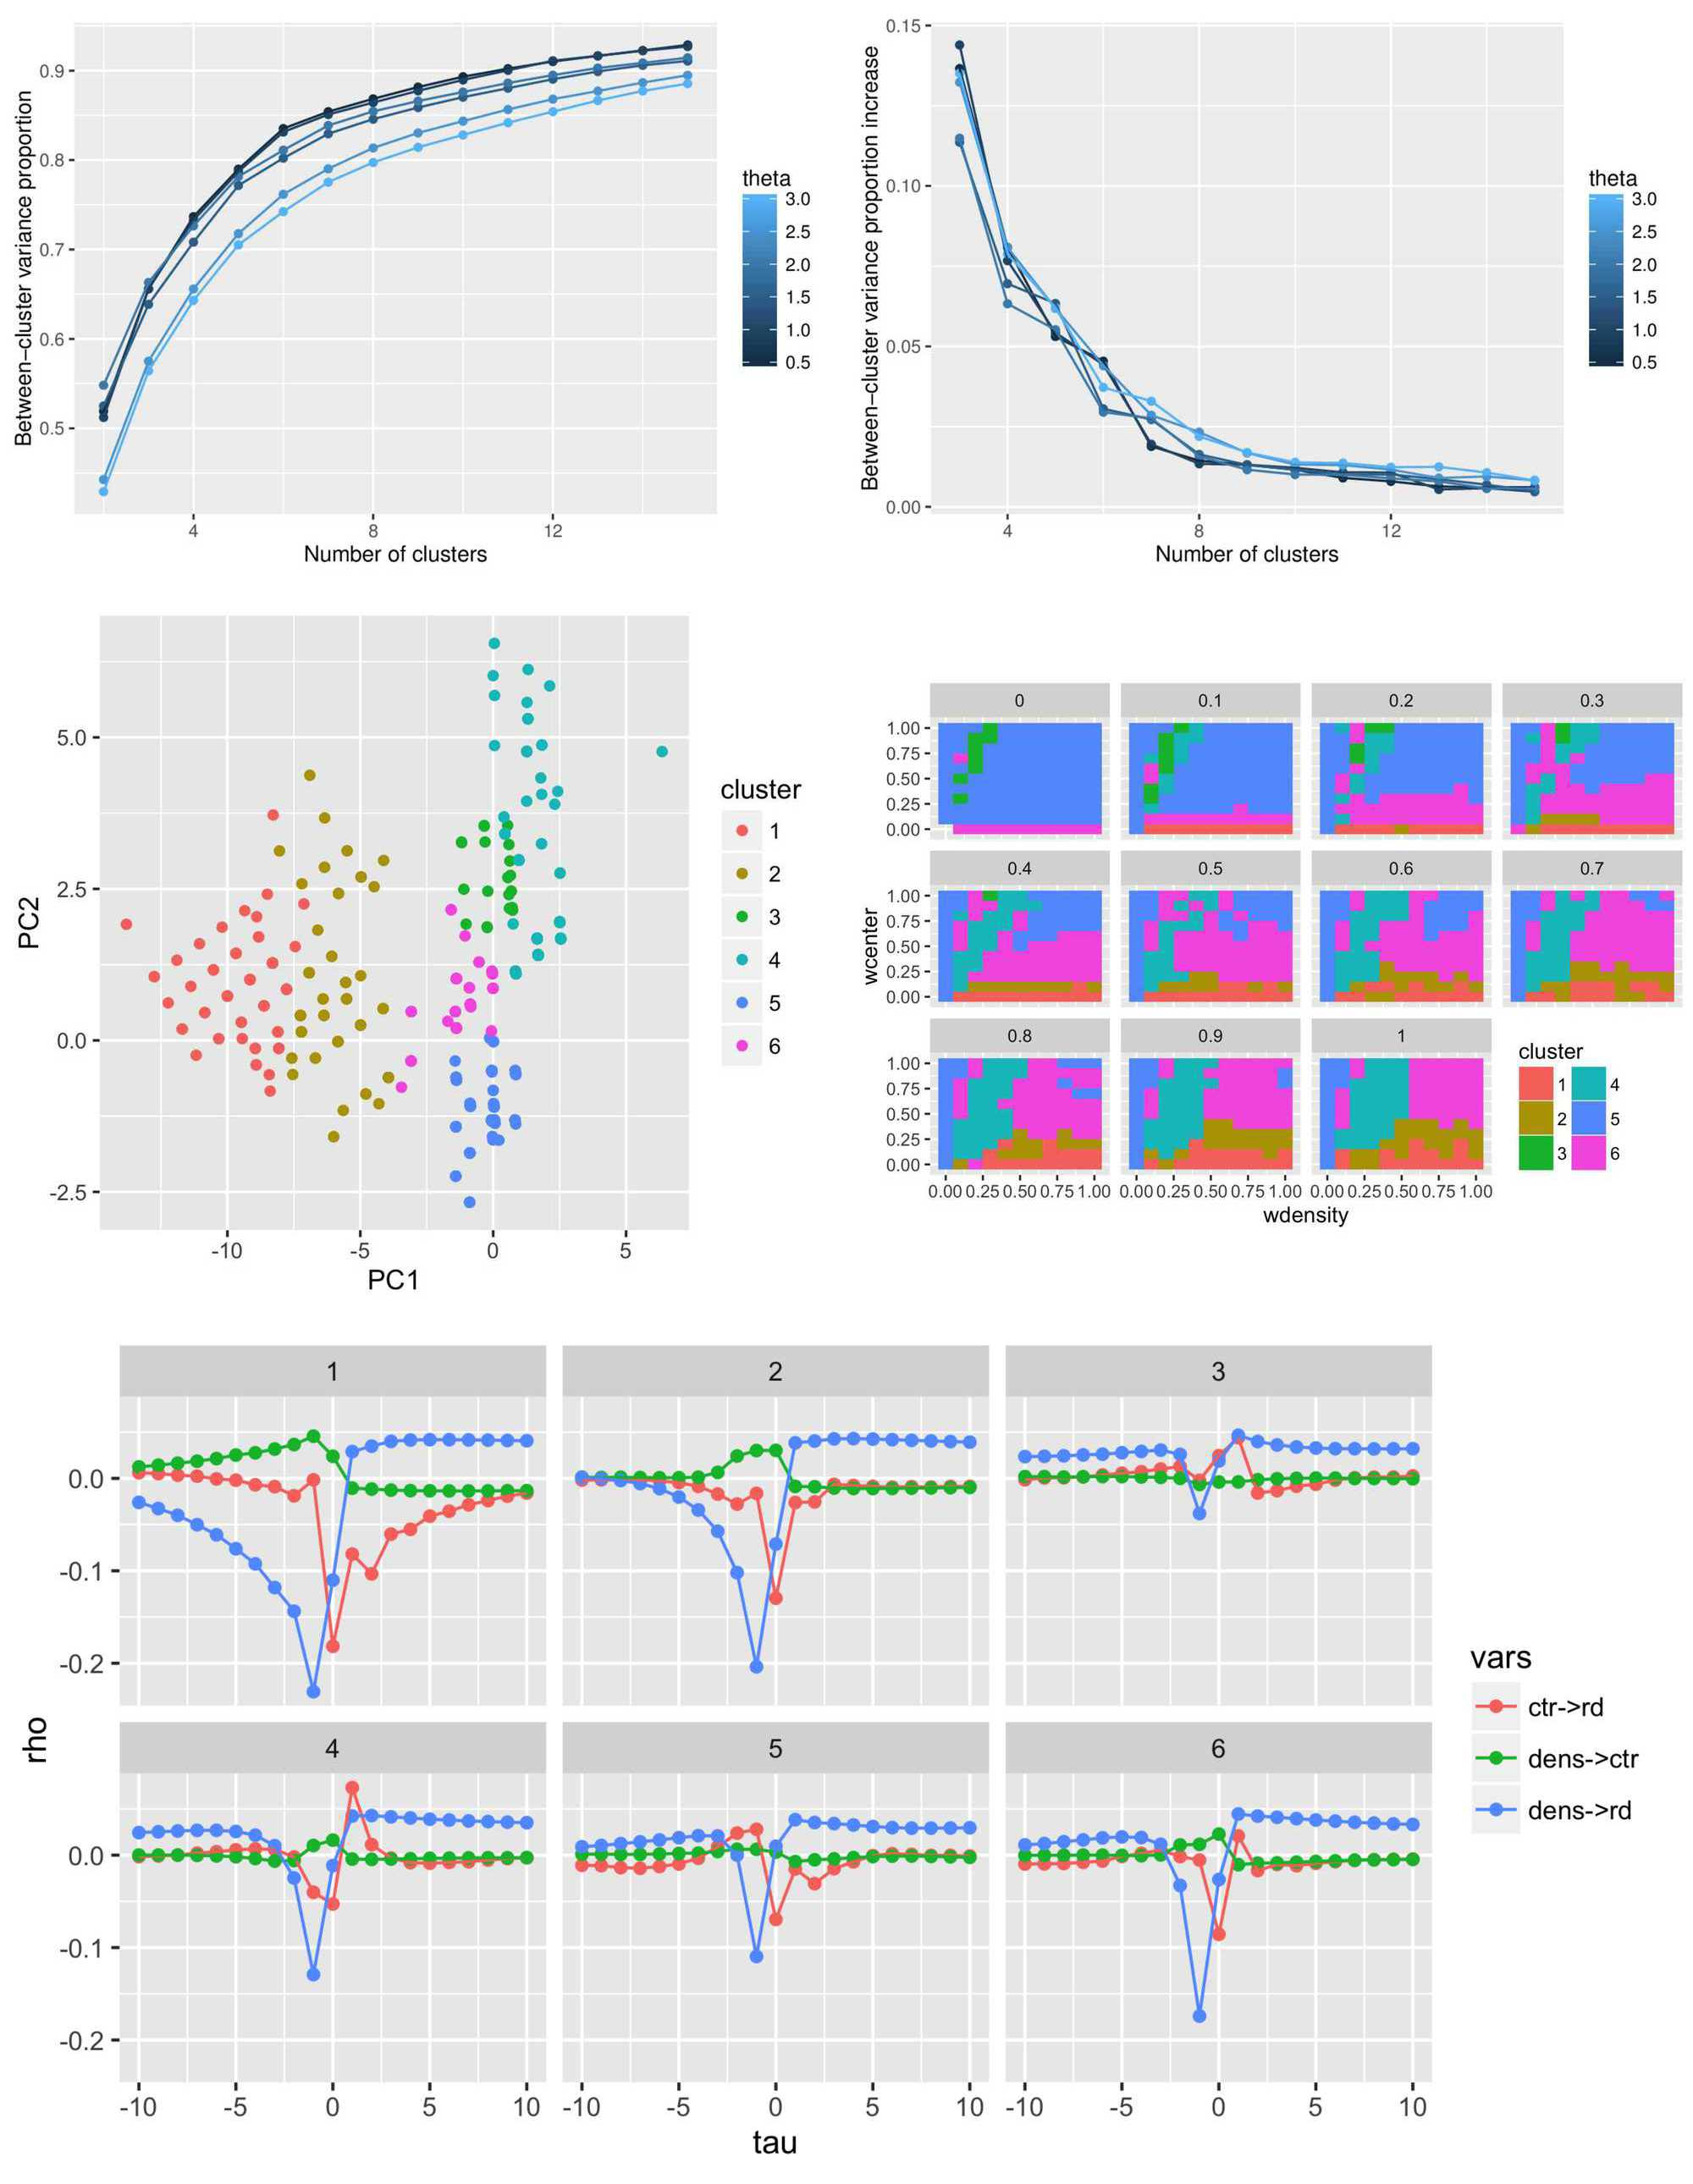
\includegraphics[width=\linewidth]{Figures/Final/4-2-2-fig-causalityregimes-clustering.jpg}
\caption[Identification of interaction regimes][Identification de régimes d'interactions]{\textbf{Identification of regimes of interaction.} \textbf{(Top left)} Inter-cluster variance as a function of cluster number. \textbf{(Top middle)} Derivative of the inter-cluster variance. \textbf{(Top right)} Features in a principal plan (81\% of variance explained by the two first components)\textbf{(Bottom left)} Phase diagram of regimes in the space $(w_{d},w_{c},w_{r})$, $w_r$ varying between the different sub-diagrams of $(w_{d},w_{c}$. \textbf{(Bottom right)} Corresponding profiles of centroids.\label{fig:causalityregimes:clustering}}{\textbf{Régimes de causalité identifiés par classification non supervisée.} (\textit{Haut}) Diagramme de phase des régimes (cluster) dans l'espace des paramètres $(w_{d},w_{c},w_{r})$, $w_r$ variant entre les différents sous-diagrammes de $(w_{d},w_{c}$. (\textit{Bas}) Trajectoires correspondantes des centroïdes, en termes de profils de corrélations retardées $\rho_{\tau}$, pour l'ensemble des couples de variables (couleur) et pour chaque cluster.\label{fig:causalityregimes:clustering}}
\end{figure}
%%%%%%%%%%%%%%%



\subsubsection{Interpretation}{Interprétation}

\bpar{
 The behavior obtained is interesting, as regions in the diagram corresponding to the different regimes are clearly delimited and connected. For example, we observe the emergence of regime 6 in which distance to network causes strongly the density in a negative way, but distance to the center causes distance to the network. Its maximal extent on $(w_d,w_r)$ is for an intermediate value $w_r=0.7$. Thus, to maximize the impact of network on density, the corresponding weight must not be maximized, what can be counter-intuitive at first sight. It illustrates the utility of the method in the case of circular causal relations difficult to entangle a priori. The regime 5, in which distance to network influences the density the same way, but the relation between distance to center and to the network is inverted, is also interesting, and predominates for low $w_r$ values. The regime 1 is an extreme one and corresponds to an isolated situation in which distance to the center has no role: this aspect dominates then totally the other interaction processes between density and network.
}{
Nous proposons finalement d'interpréter les régimes obtenus, représentés en Fig.~\ref{fig:causalityregimes:clustering}. Le comportement obtenu est particulièrement intéressant : les régions du diagramme de phase selon les paramètres correspondant aux régimes sont clairement délimitées et connexes. Par exemple, on observe l'émergence d'un régime (numéroté 1) où la densité cause fortement la distance au réseau de manière négative (au sens de l'existence d'un $\rho_+$ négatif), mais la distance au centre cause la distance au réseau, régime dont l'étendue maximale dans le plan $(w_d,w_c)$ est pour une valeur intermédiaire $w_r=0.7$. Ainsi, pour maximiser l'impact du réseau sur la densité, il ne faut pas maximiser le poids correspondant mais prendre une valeur intermédiaire, ce qui peut paraître contre-intuitif en premier abord : cela illustre l'intérêt de la méthode dans le cas de relations circulaires difficiles à démêler a priori. Le régime 2, où la distance au réseau influence la densité de la même manière, mais la relation entre distance au centre et route est inversée, est prédominant dans les faibles $w_r$ : ainsi, l'attenuation du rôle de la distance à la route conduit le centre à inverser sa relation avec la distance à la route. Le régime 6, extrême quant à sa position dans l'espace des paramètres car dans un voisinage de $w_c = 0$, correspond à une situation isolée dans laquelle la distance au centre n'importe pas comme variable explicative, et on observe une causalité de la densité sur la distance au centre ($\rho_+$ pour $D\rightarrow R$) et de la distance à la route sur la distance au centre ($\rho_-$ pour $C\rightarrow R$), c'est-à-dire que cet aspect est totalement dominé par les autres.
}



\bpar{
This application on synthetic data demonstrate on one hand the robustness of the method given the consistence of obtained regimes, and realizes this way a much more finer qualification of model behavior than the one done in the original paper. In this precise case, it can be taken as an instrument of knowledge for relations between networks and territories in itself, allowing the test of assumption or the comparison of processes in the stylized model.
}{
Cette application sur données synthétiques démontre ainsi d'une part la robustesse de la méthode vu la cohérence des régimes obtenus, et constitue aussi une qualification beaucoup plus précise des comportements du modèle que celle réalisée dans l'article initial. Dans ce cas précis, il peut s'agir d'un instrument de connaissance des relations entre réseaux et territoires en lui-même, permettant le test d'hypothèses ou la comparaison de processus dans le modèle stylisé.
}










%--------------------------------------------------------









%%%%%%%%%%%%%%%%%%%%%%%
\subsection{Network-territory relations in South Africa}{Relations Réseaux-territoires en Afrique du Sud}



\bpar{
We assum that territorial dynamics and network dynamics responded differently to these. We expect to learn from these project informations on interactions at long time scale and large spatial scale, in a very particular context of constrained growth.
}{
Nous démontrons à présent les potentialités de notre méthode à établir des liens entre variables sur des données géo-historiques sur le temps long, pour le cas du réseau ferré en Afrique du Sud au cours du 20ème siècle. En faisant l'hypothèse que les territoires et les réseaux réagissent différemment aux événements historiques, les motifs de causalité devraient informer sur leur relations sur le temps long.
}


\subsubsection{Context}{Contexte}


\bpar{
Transportation Networks can be leveraged as a powerful socio-economic control tool, with even more significant outcomes when it percolates to their interaction with territories. The case of South Africa is an accurate illustration, as \cite{baffi:tel-01389347} shows that during apartheid railway network planning was used as a racial segregation tool by shaping strongly constrained mobility and accessibility patterns. In particular, it is shown qualitatively that dynamics between territories and networks profoundly changed at the end of the apartheid, transforming a tool of planed segregation (network shaped was optimized to minimize unwanted accessibility) into an integration tool thanks to recent changes in network topology patterns. We propose to investigate the potential \emph{structural} properties of this historical process, by focusing on dynamical patterns of interactions between the railway network and city growth. More precisely, we try to establish if the segregative planning policies did actually modify the trajectory of the coupled system, what would correspond to deeper and wider impacts. 
}{
Les réseaux de transport peuvent être utilisés comme un puissant outil de contrôle des populations, avec des effets encore plus significatifs lorsque ceux-ci perturbent les relations avec les territoires. Le cas de l'Afrique du Sud est une illustration pertinente, puisque \cite{baffi:tel-01389347} montre que lors de l'apartheid la planification du réseau ferré était utilisée comme un outil de ségrégation raciale par l'établissements de motifs de mobilité et d'accessibilité fortement contraints\footnote{La politique de ségrégation est interprétée par~\cite{baffi:tel-01389347} (p.~189) comme une intention de ``connecter sans connectivité'', conjointement avec les migrations forcées de la population ségréguée dans des zones spécifiques à l'écart des fonctions urbaines, appelées \emph{bantoustans}. Le réseau a alors été spécifiquement développé pour relier ceux-ci aux zones de production sans les connecter efficacement aux centres urbains.}. En particulier, il est montré qualitativement que les dynamiques entre réseaux et territoires ont profondément changé à la fin de l'apartheid, transformant un outil de ségrégation planifiée (une forme de réseau conçue pour minimiser l'accessibilité des populations ségréguées) en un outil d'intégration grâce à des changement récents dans la topologie du réseau. Nous étudions ici les potentielles propriétés \emph{structurelles} de ce processus historique, en se concentrant sur les motifs dynamiques des interactions entre le réseau ferré et la croissance des villes. Plus précisément, nous essayons d'établir si les politiques de planification ségrégatives ont effectivement modifié la trajectoire du système couplé, ce qui correspondrait à des impacts plus larges et profonds que leurs effets immédiats.
}



\subsubsection{Data}{Données}


\bpar{
We use a comprehensive database covering the full South African railway network from 1880 to 2000 with opening and closing dates for each station and link, together with a city database spanning from 1911 to 1991 for which consistent ontologies for urban areas have been ensured. These database are described by~\cite{baffi:tel-01389347}, but they are not open so we make available only the aggregated data we used in the analysis.
}{
Nous utilisons une base de données complète couvrant l'ensemble du réseau ferré Sud-Africain de 1880 à 2000 avec les dates d'ouverture et de fermeture pour chaque station et liaison, couplée à une base de données pour les villes s'étendant de 1911 à 1991 pour laquelle des ontologies consistantes pour les aires urbaines ont été assurées. Ces bases de données sont décrites par~\cite{baffi:tel-01389347}, mais ne sont pas ouvertes. Pour respecter notre exigence d'ouverture, nous ne mettons ainsi à disposition que les données agrégées utilisées dans l'analyse.
}



\subsubsection{Network Measures}{Mesures de réseau}

\bpar{
First, a dynamical study of network measures seem to confirm the hypothesis: a trend rupture in closeness centrality (defined for a node as the average travel time to other nodes) at a roughly constant network size evolution, at a date corresponding to the beginning of official segregative policies, suggests that the planning process after this date had in the best case no global effect on network performance, and in the worst case had intended negative effects on accessibility with the aim to physically segregate more.
}{
Une analyse préliminaire consiste à regarder l'évolution dynamique des mesures de réseau, celles-ci pouvant témoigner de ruptures dans les propriétés structurelles du réseau et donc de mutations historiques profondes. L'évolution de certaines propriétés du réseau, comme les distributions de la centralité ou de l'accessibilité, peut témoigner de l'existence d'une planification les ayant influencées. Nous montrons en Fig.~\ref{fig:causalityregimes:network} l'évolution des mesures de réseau dans le temps\footnote{Globalement, \cite{baffi:tel-01389347} (p.~154) montre que le réseau ferré sud-africain s'est développé en arborescence et que les politiques de ségrégation ont figé sa structure, l'empêchant de mailler le territoire.}, correspondant à certaines des mesures définies en~\ref{sec:staticcorrelations}. La centralité de proximité, que nous définissons comme le temps moyen de trajet vers les autres noeuds, présente un comportement intéressant. En effet, la taille du réseau et les valeurs moyennes des centralités présentent un comportement concordant, qui correspond à l'expansion initiale du réseau. Par contre, la tendance de la hiérarchie de la centralité de proximité à se réduire est soudainement rompue à la date correspondant à l'officialisation des politiques ségrégatives en 1951, alors que taille et forme géométrique globale du réseau, traduites par l'efficience, restent constants. Ainsi, dans le meilleur des cas la planification après cette date est une coincidence avec la variation de cette propriété. Il est très probable qu'elle soit en effet responsable de cette rupture de tendance, c'est-à-dire a eu les effets escomptés sur l'accessibilité, dans le but d'empêcher la diminution de la ségrégation, puisque plus la hiérarchie est faible plus le réseau est égalitaire.
}


%%%%%%%%%%%%%%
\begin{figure}[h!]
%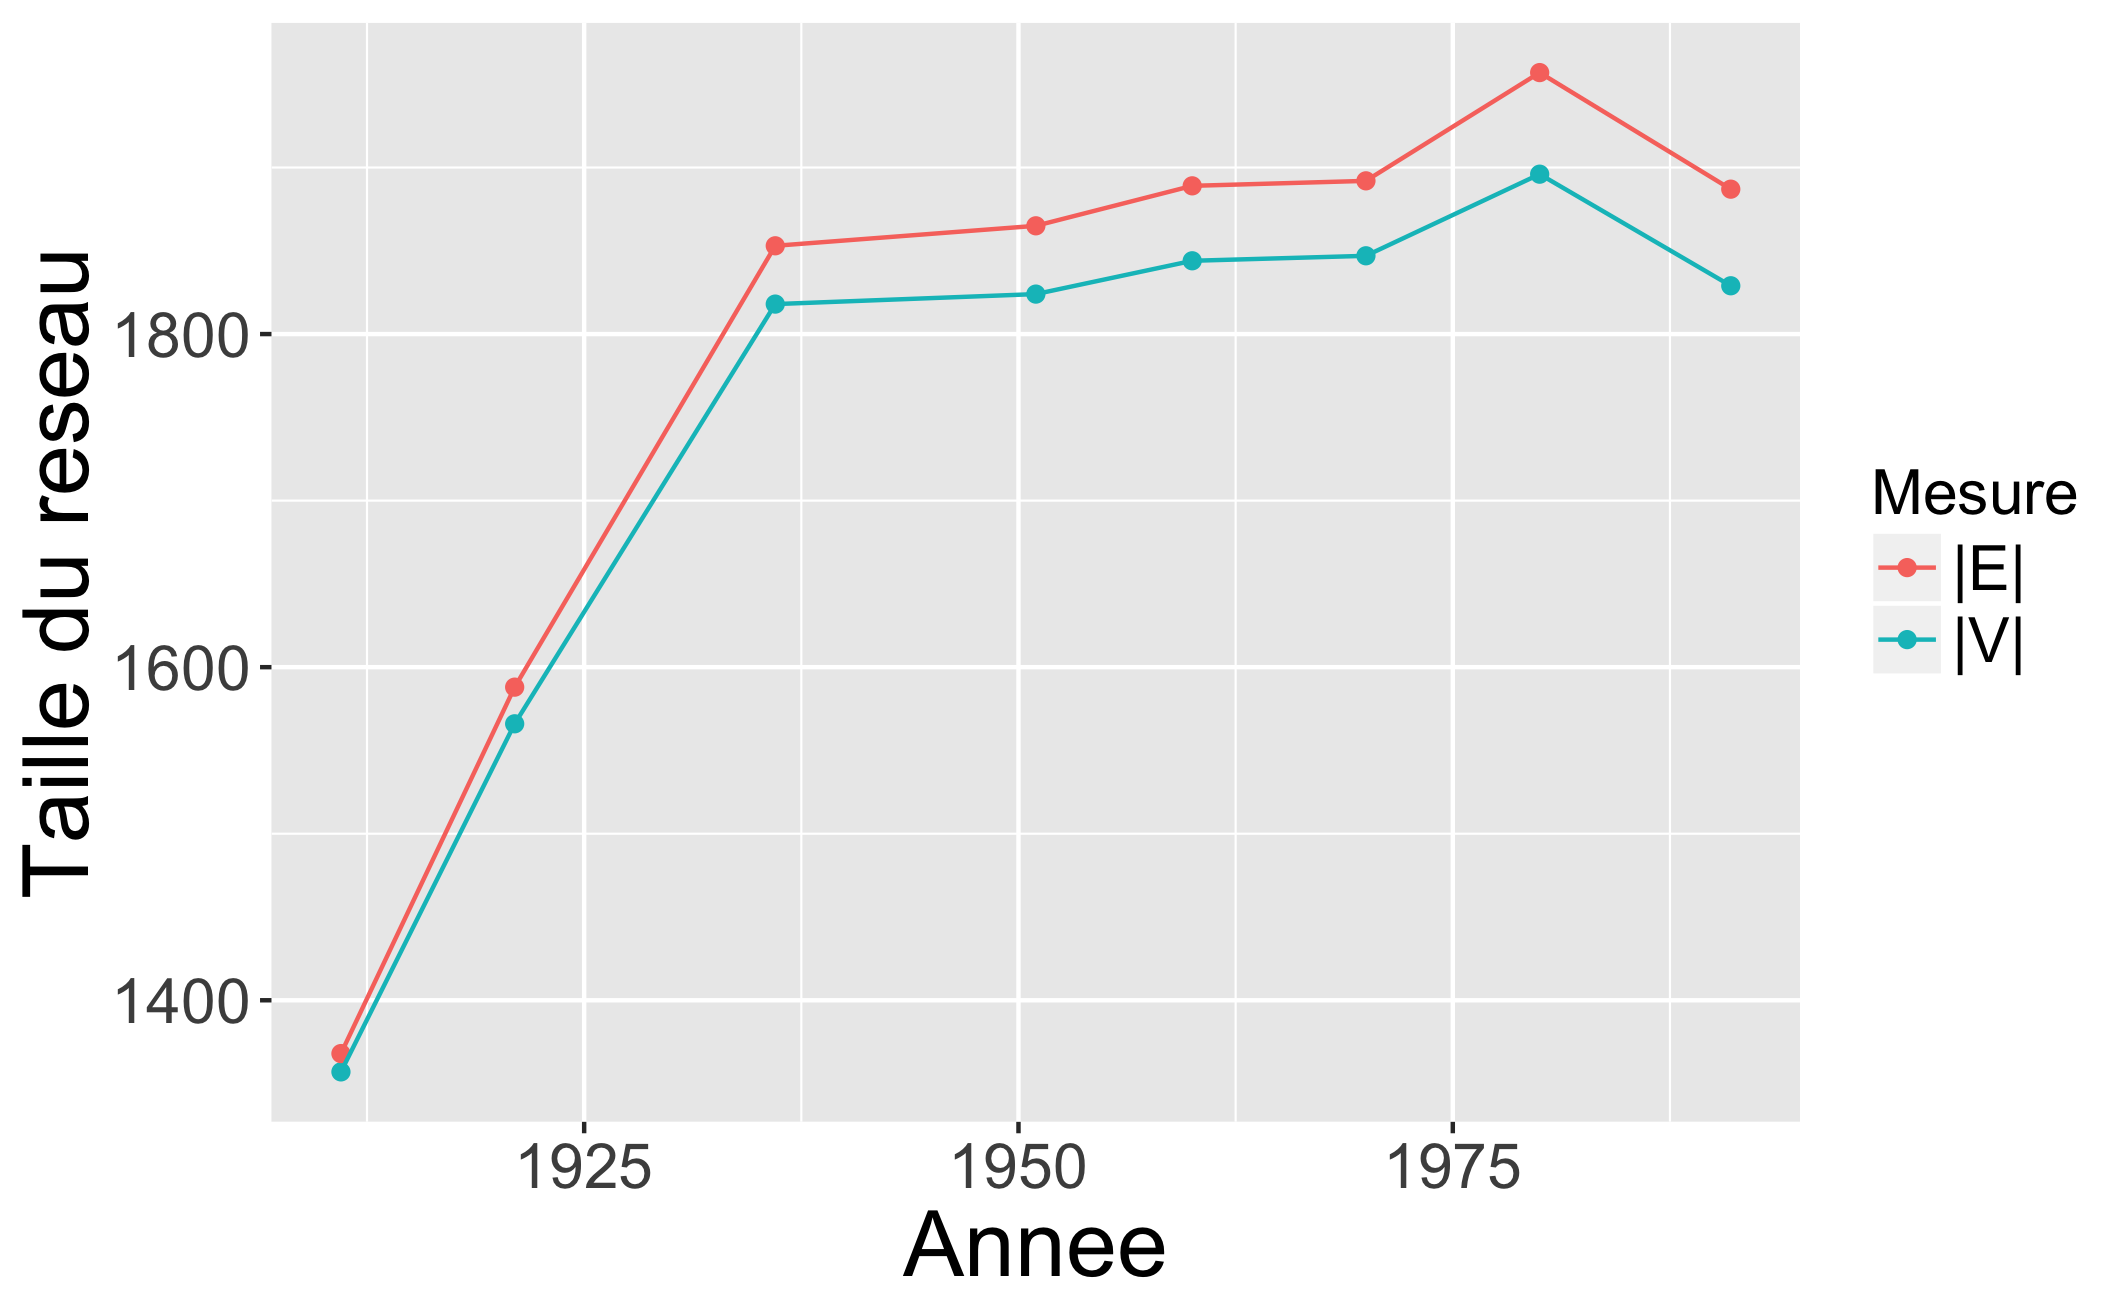
\includegraphics[width=0.42\linewidth]{Figures/CausalityRegimes/nw_nwSize}
%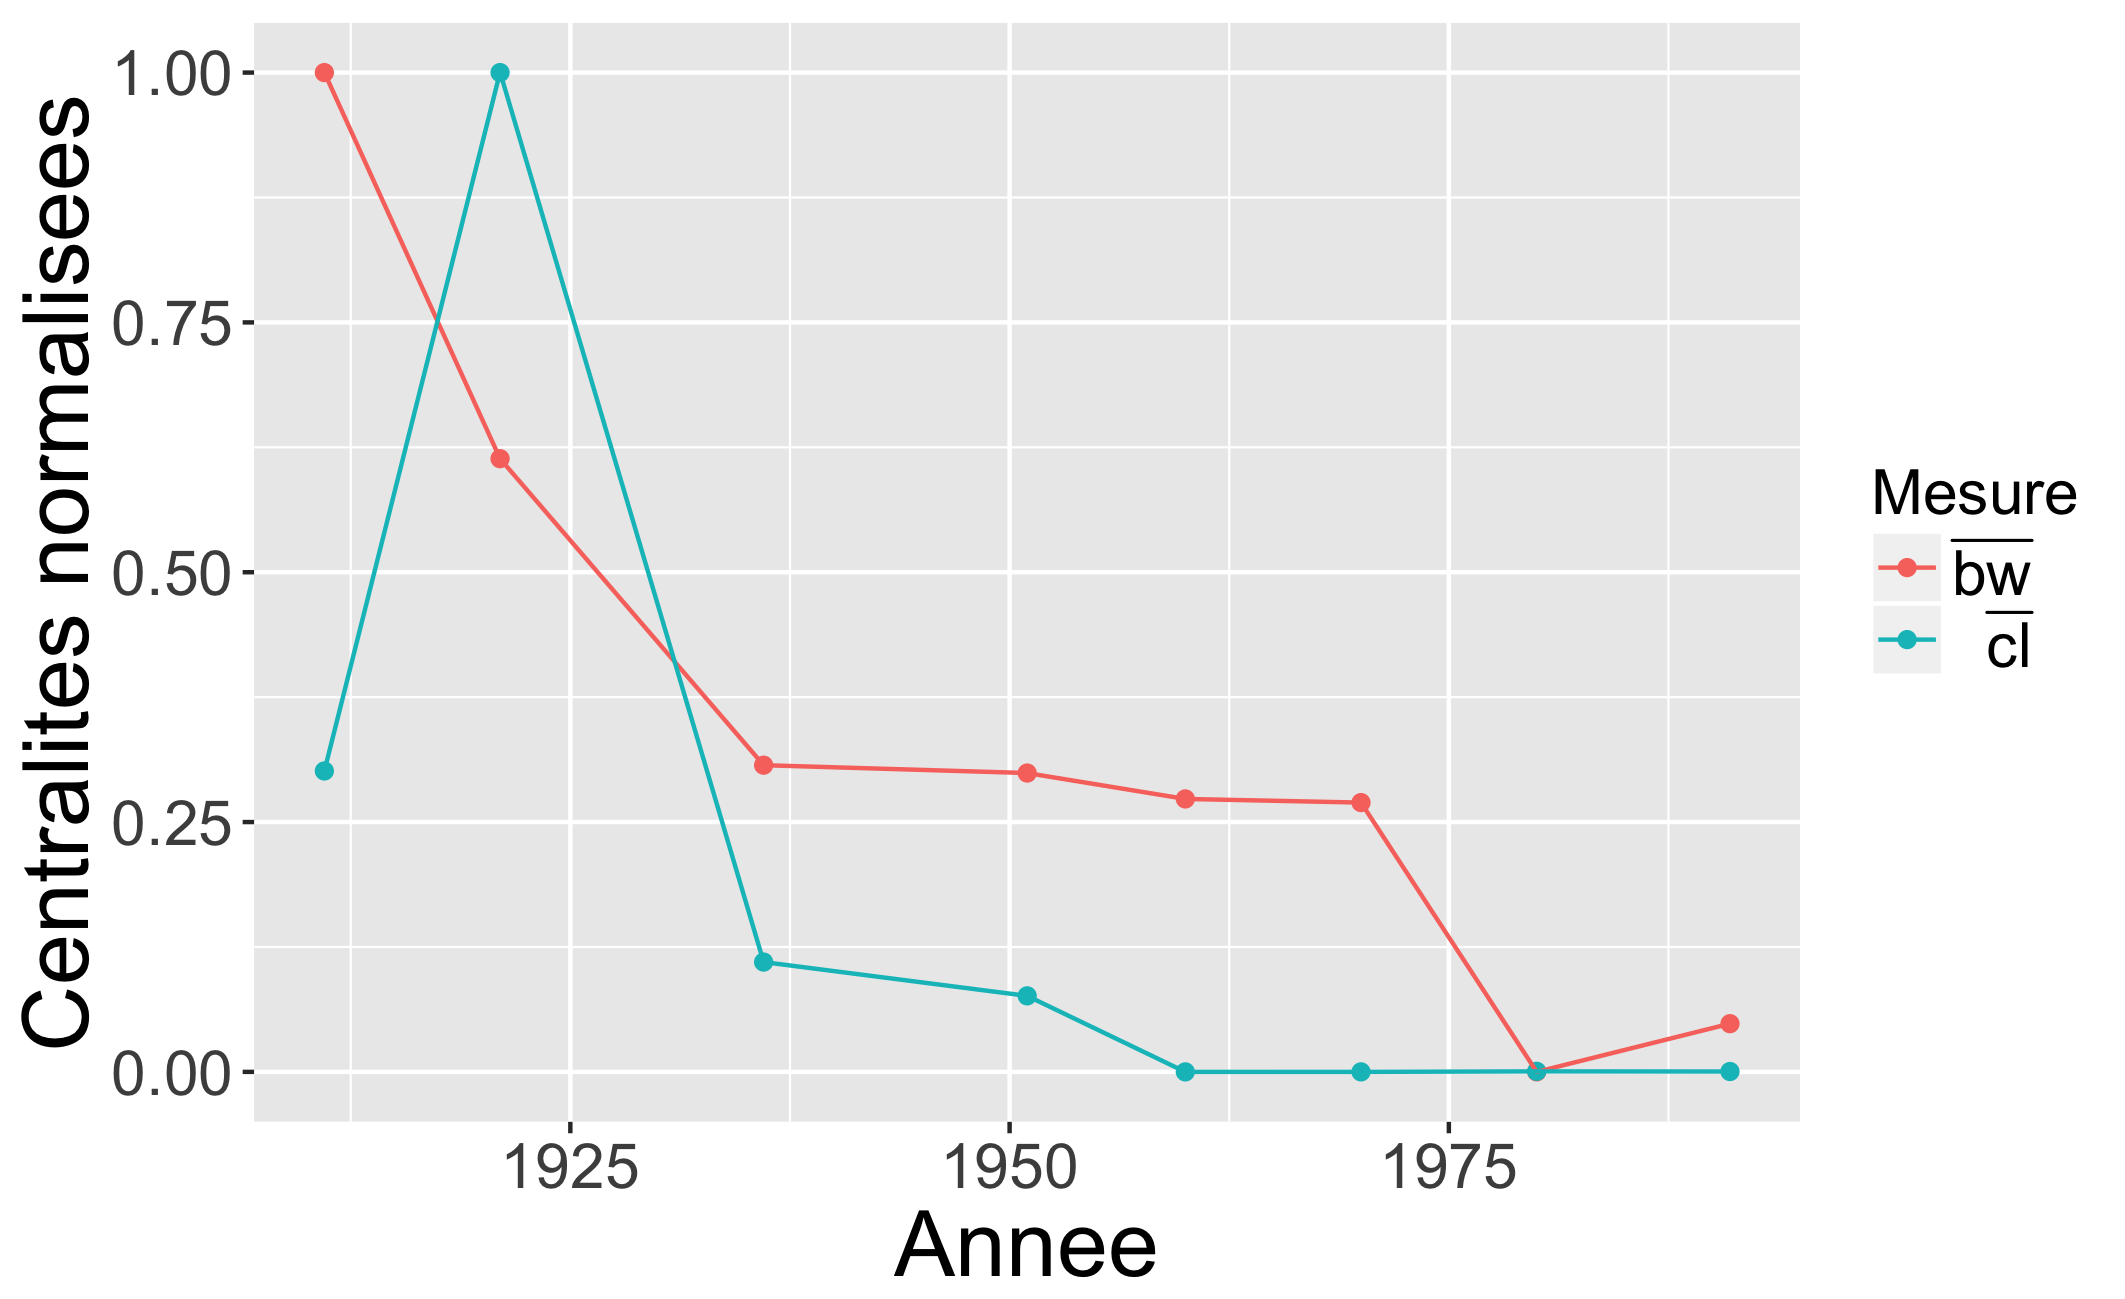
\includegraphics[width=0.47\linewidth]{Figures/CausalityRegimes/nw_meanCentralities}\\
%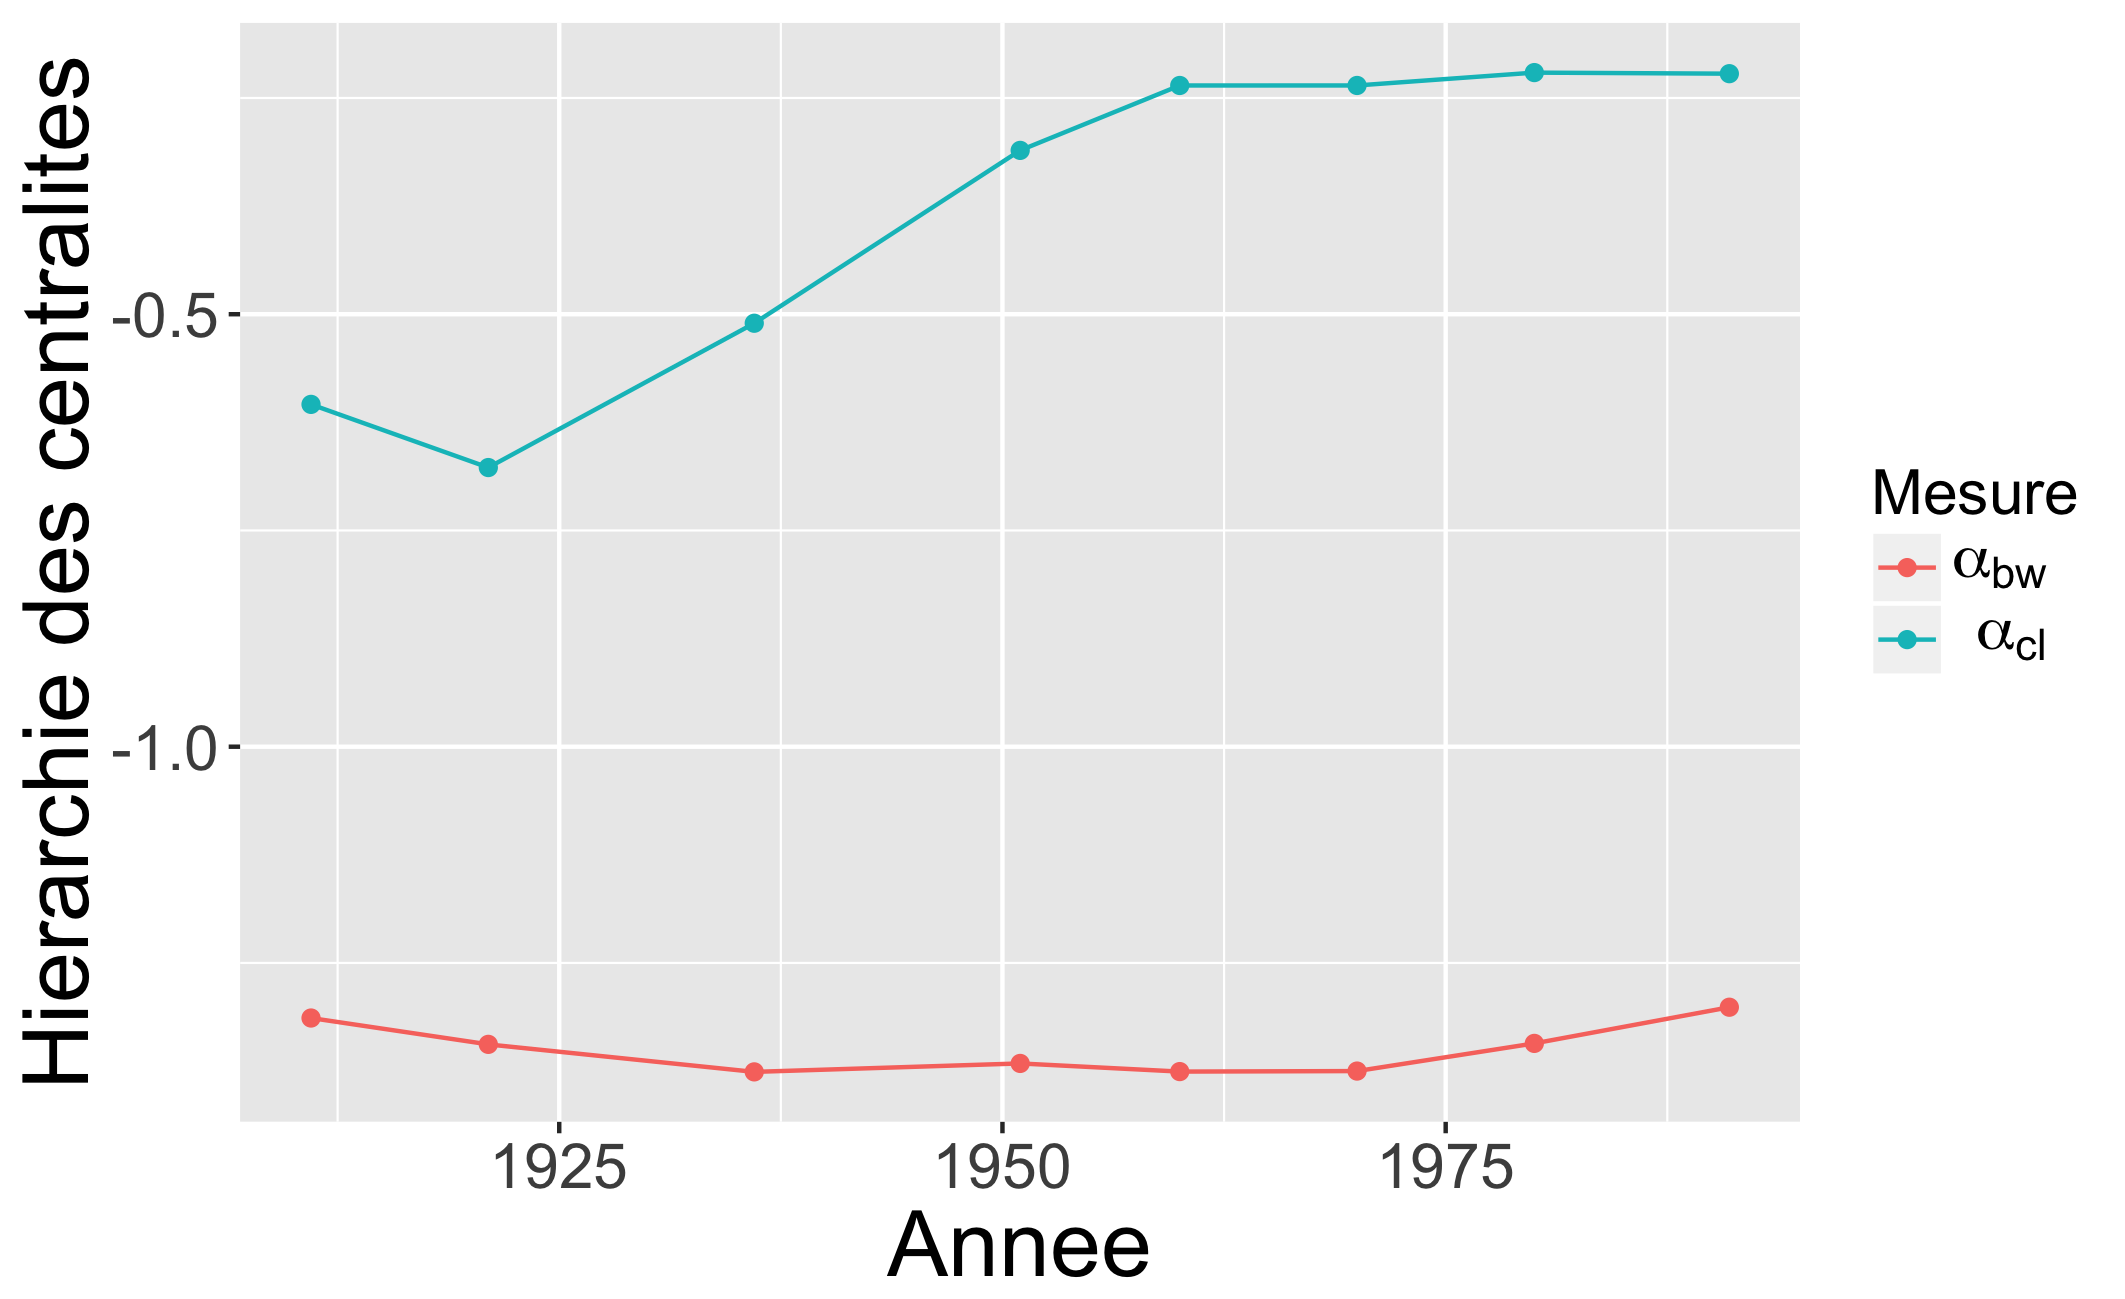
\includegraphics[width=0.48\linewidth]{Figures/CausalityRegimes/nw_hierarchies}
%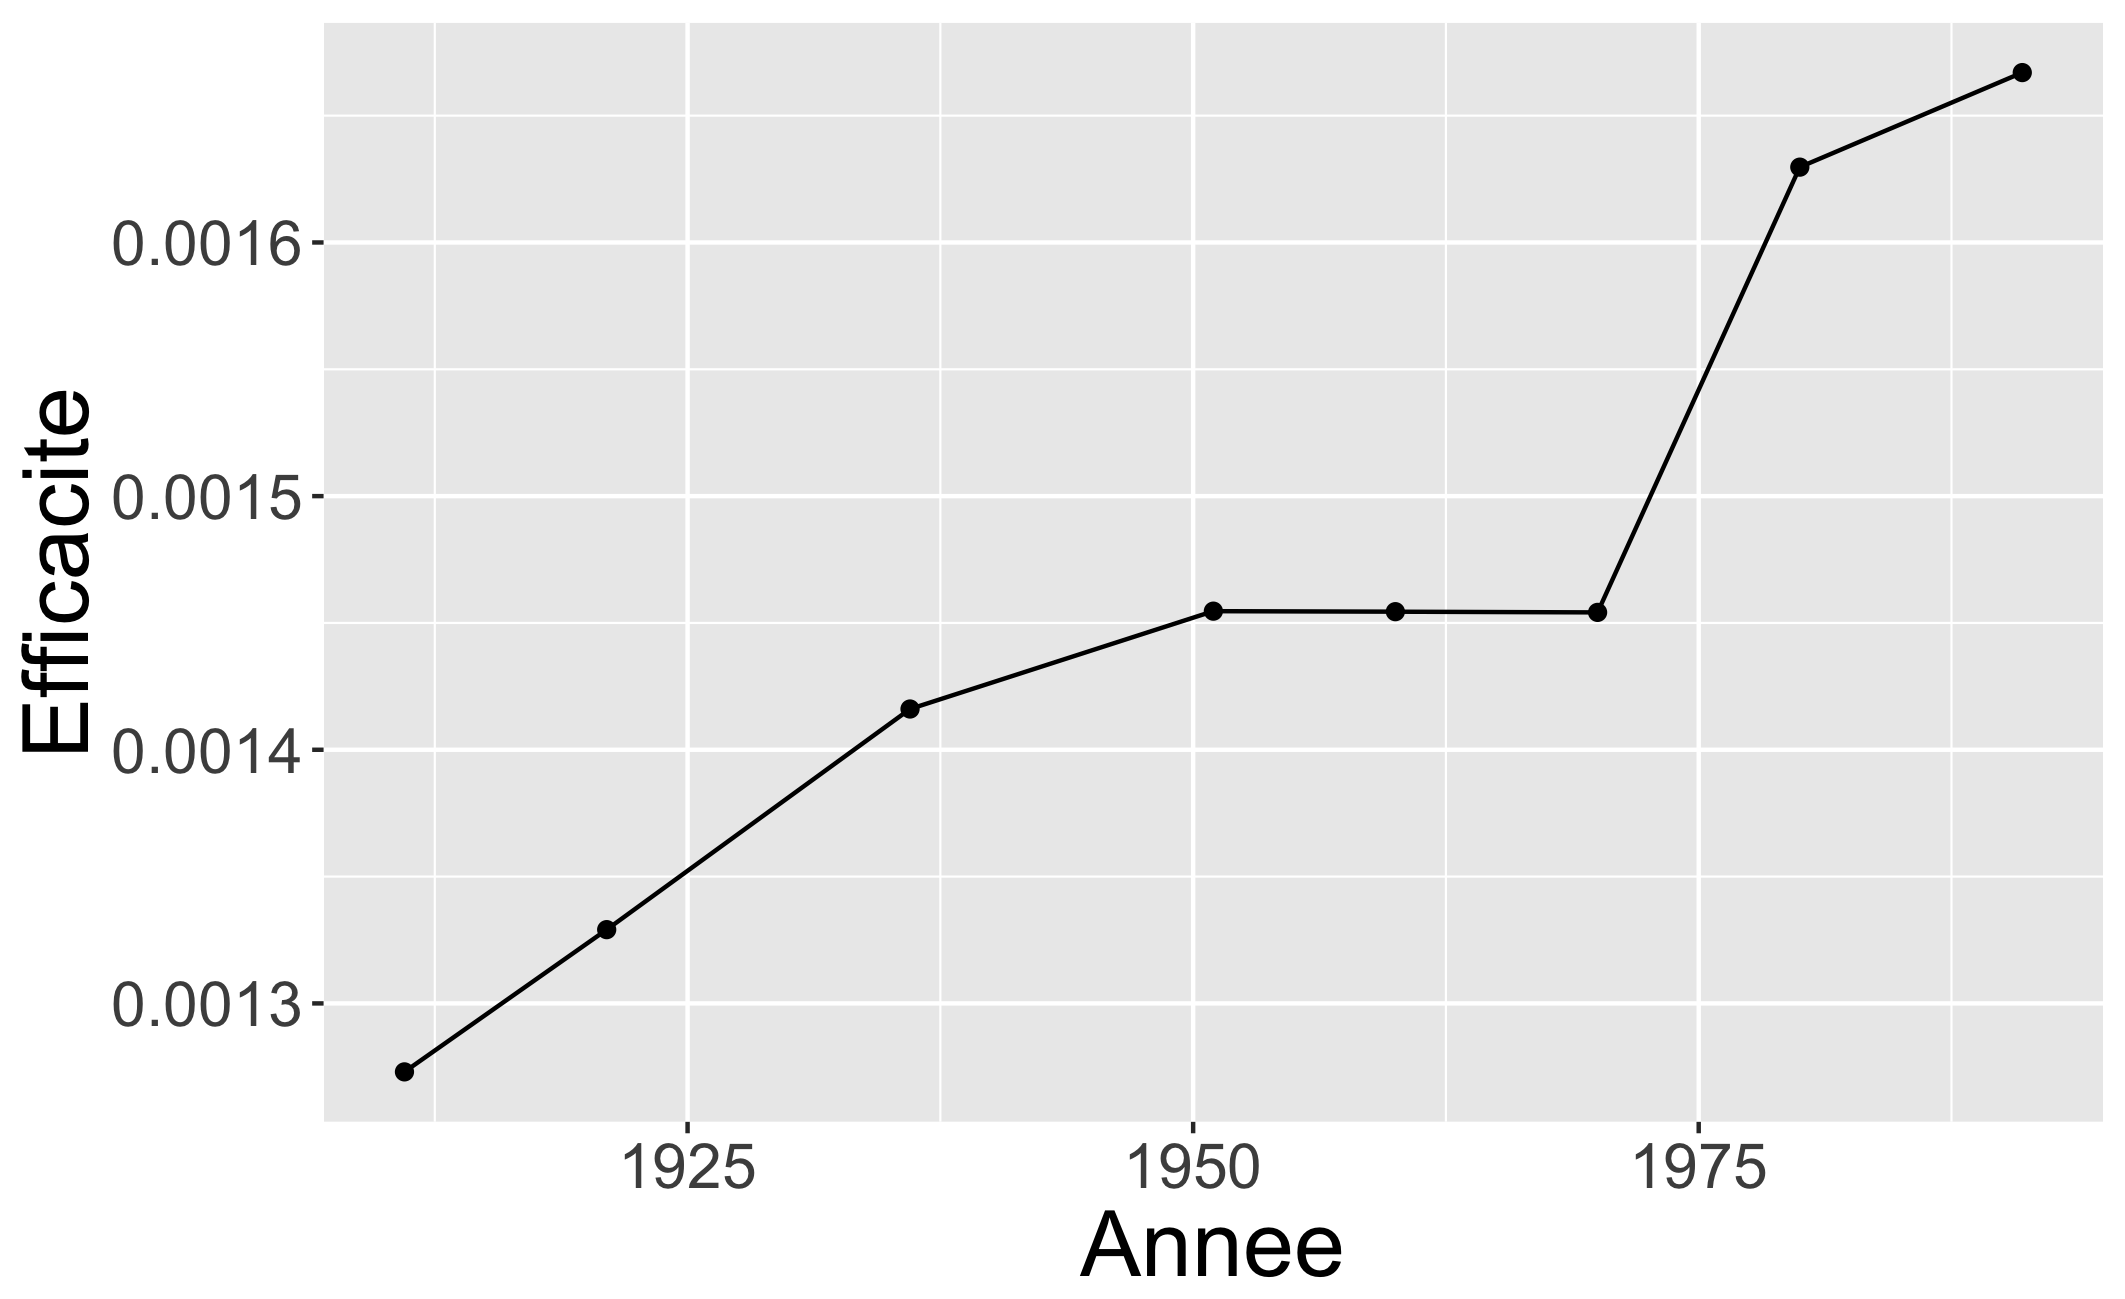
\includegraphics[width=0.41\linewidth]{Figures/CausalityRegimes/nw_efficiency}
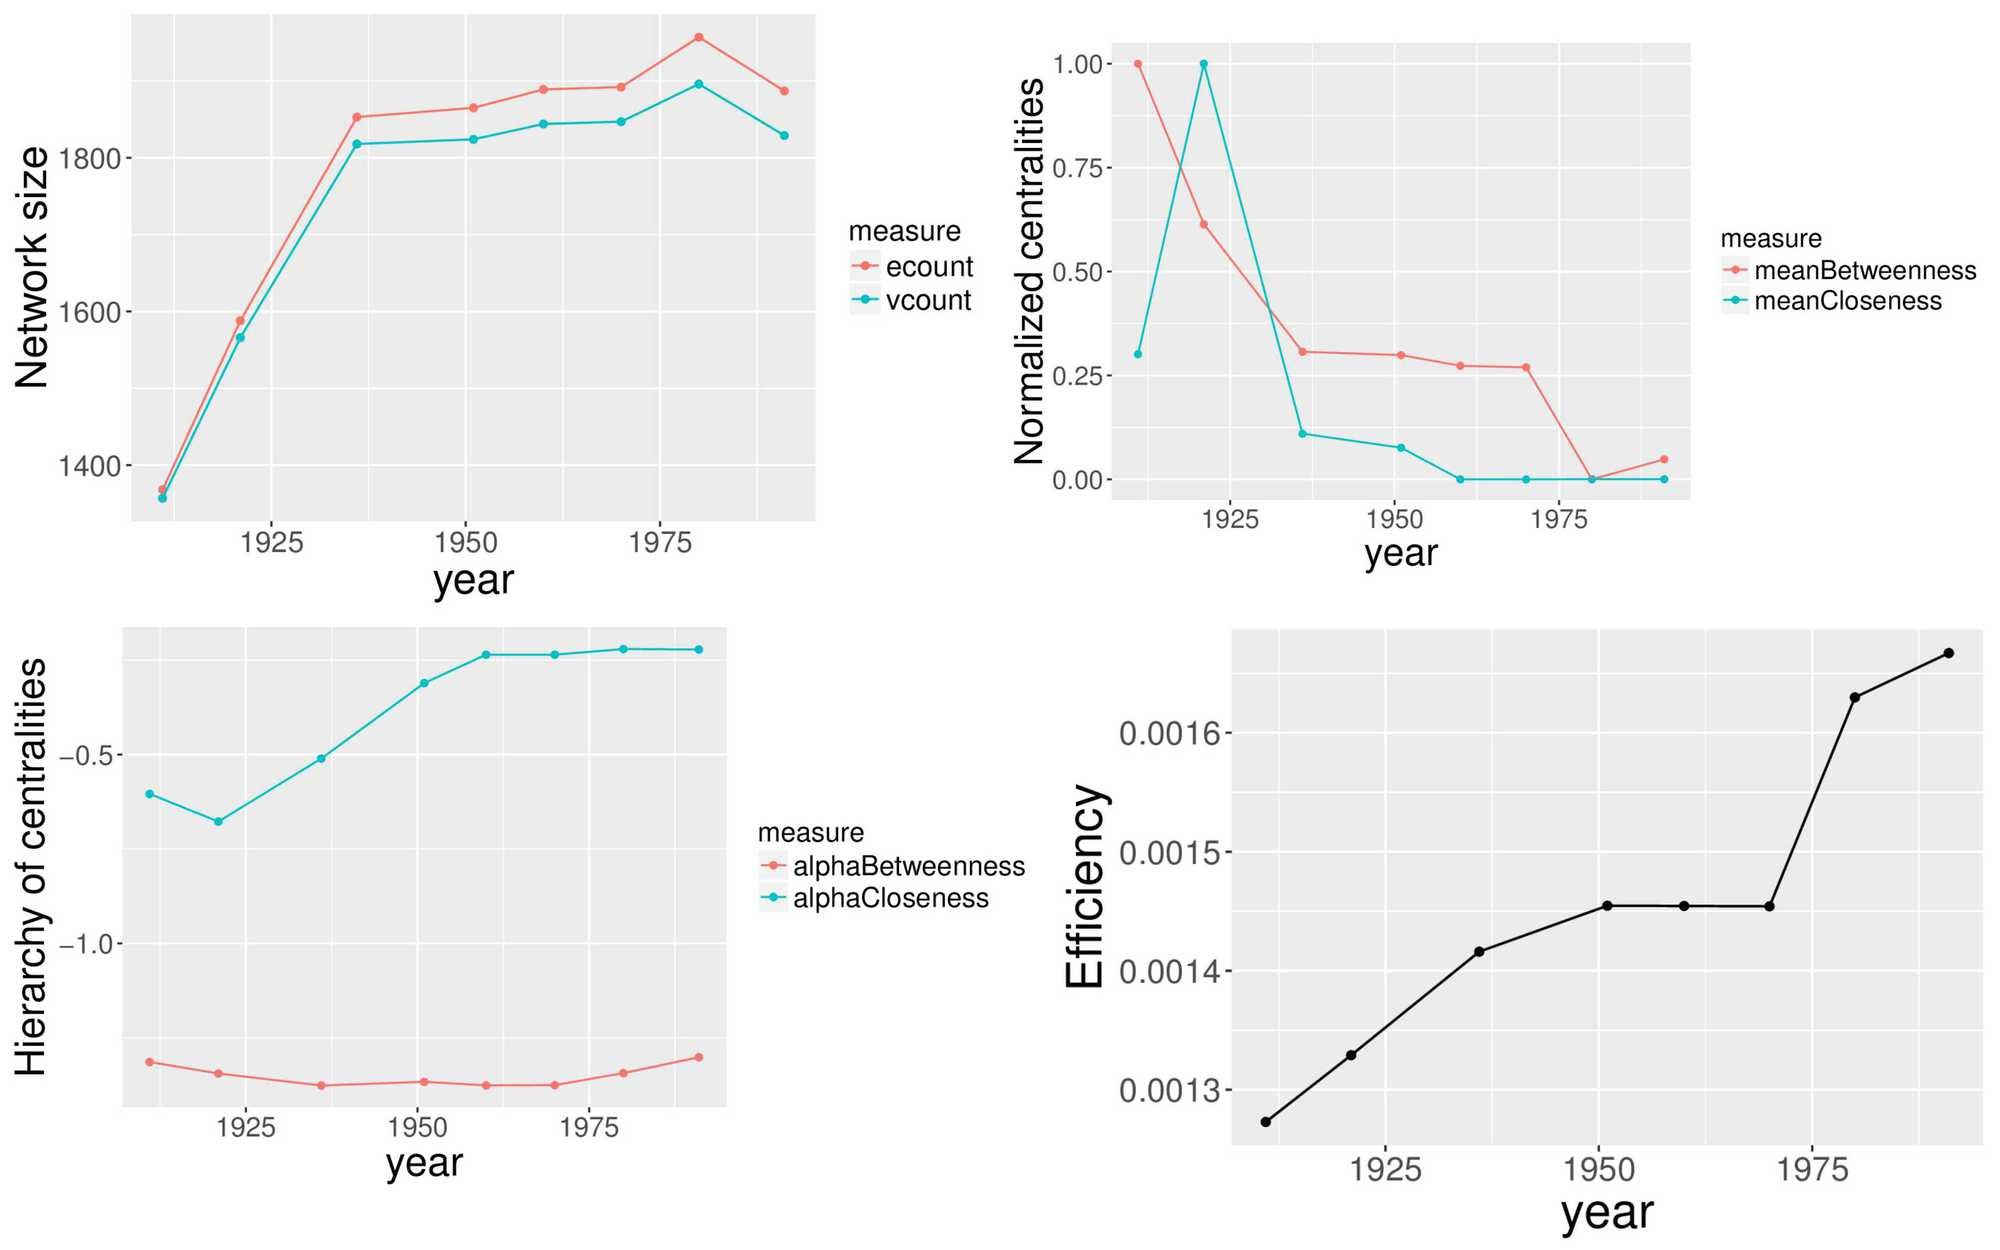
\includegraphics[width=\linewidth]{Figures/Final/4-2-3-fig-causalityregimes-network.jpg}
\caption[Evolution of network measures][Évolution des mesures du réseau ferré sud-africain]{\label{fig:causalityregimes:network}}{\textbf{Évolution des mesures du réseau ferré sud-africain.} On calcule pour l'ensemble des dates les mesures basiques de réseau : taille, centralités résumées par leur hiérarchie et leur moyenne, efficience. Les centralités sont normalisées pour comparaison de leur variation respective ($\max \bar{bw} = 0.07$, $\max \bar{cl} = 1.5e-4$).\label{fig:causalityregimes:network}}
\end{figure}
%%%%%%%%%%%%%%



\subsubsection{Causality patterns}{Motifs de causalité}


\bpar{
We then turn to dynamical interactions between the railway network and city growth. For that, we study Granger causalities, in the large sense of correlations between lagged variables, estimated between cities growth rates and accessibility differentials due to network growth, for all cities and urban areas having a connection to the network.
We test both travel-time and population weighted accessibilities, for varying values of distance decay parameter. Lagged correlations are fitted on varying length time windows, to test for potentially varying stationarity scales.
}{
Nous examinons à présent les interactions dynamiques entre le réseau ferré et la croissance urbaine. Pour cela, nous appliquons la méthode développée dans la première partie, qui consiste à l'étude des causalités de Granger, au sens large des corrélations entre les variables retardées, estimées entre les différentiels de population des villes et les différentiels d'accessibilité dus à la croissance du réseau, pour toutes les villes ou aires urbaines ayant une connection au réseau. Nous testons à la fois l'accessibilité en termes de distance et pondérée par la population à l'origine et aux deux extrémités. Si $P_i$ sont les populations, $d_{ij}$ la matrice de distance dans le réseau, l'accessibilité de $i$ sera donnée par $Z_i = w_i \sum_j w_j \exp \left(- d_{ij} / d_0 \right)$ où $d_0$ est le paramètre de décroissance et les poids $w_i$ sont $1/N$ ou $P_i / \sum_j P_j$ selon la modalité. Nous faisons varier les valeurs de $d_0$ pour prendre en compte les relations à différentes échelles spatiales. De plus les corrélations retardées sont estimées sur des fenêtres temporelles de taille variable $T_W$, pour tester différentes échelles potentielles de stationnarité temporelle.
}

% rq : should test log returns of variables ?

\bpar{
Results are shown in Figure~\ref{fig:causalityregimes:sudafcorrs}. We find that results are significant with travel-time accessibility only, autocorrelation dominating with weighted accessibility. A time-window of 30 years appears to be a good compromise between the number of significant correlations ($p<0.1$ for a Fisher test) and the absolute correlation level across all lags and distance decays, what should correspond roughly to the time-stationarity scale of the system. We observe furthermore a phase transition when distance decay increases, revealing the shift between the spatial scale of urban areas and the scale of the country, what gives local spatial stationarity scale.
}{
Les résultats des estimations sont montrés en Figure~\ref{fig:causalityregimes:sudafcorrs}. Nous obtenons des résultats significatifs avec l'accessibilité non-pondérée seulement, que nous montrons ici\footnote{Nous donnons en Annexe~\ref{app:sec:causalityregimes}, Fig.~\ref{fig:app:causalityregimes:sudafcorrs} les profils de corrélations retardées estimées pour les accessibilités pondérées à l'origine et à l'origine et à la destination. L'auto-corrélation domine a priori l'accessibilité pondérée : en effet, on a pour les deux variables pondérées des valeurs positives pour les faibles valeurs de $d_0$ uniquement, les autres n'étant pas significatives.}. Le meilleur compromis pour la fenêtre temporelle apparaît être une trentaine d'année, si on cherche à avoir à la fois un bon nombre de corrélations significatives (définies par $p<0.1$ pour un test de Fisher) et un niveau moyen élevé de corrélation absolue sur l'ensemble des retards et des paramètres de décroissance. Nous interprétons cette valeur comme approximativement l'échelle spatiale de stationnarité du système. Il s'agirait de la durée sur laquelle un régime du système urbain est relativement stable, et est du même ordre de grandeur que la durée de l'apartheid. 

 De plus, le nombre de corrélations significatives présente clairement une transition de phase dans ses valeurs intermédiaires en fonction de $d_0$ (Fig.~\ref{fig:app:causalityregimes:sudafcorrs}), ce qui devrait correspondre au passage entre l'échelle spatiale des aires urbaines et celle du pays, et donne ainsi l'échelle locale de stationnarité spatiale, autour de $d_0 = 500km$. Les villes du Cap et de Johannesburg sont à 1400km de distance et correspondent à deux régions aux extrémités du pays : cette échelle est donc une échelle régionale, inférieure à celle du système urbain du pays.
}


\bpar{
We obtain therethrough clear causality patterns, namely an inversion of the Granger causality (lagged correlation up to 0.5 for several values of distance decay), from accessibility causing population growth with a lag of 10-20 years before the apartheid (1948), to the opposite after the apartheid (lag 20 years). We interpret these as \emph{Structural segregation}, i.e. a significant impact of planning policies on dynamics of interactions between networks and territories. Indeed, the first regime corresponds to direct effect of transportation on migrations in a free context in opposition to the second one.
}{
L'examen du comportement des corrélations retardées en Fig.~\ref{fig:causalityregimes:sudafcorrs} conduit à l'observation de motifs de causalité assez clairs, puisque le sens de la causalité de Granger s'inverse autour de 1950, celle-ci étant à chaque fois marquée par des corrélations allant jusqu'à 0.5 pour certaines valeurs du paramètre de décroissance. On passe ainsi d'une accessibilité causant la croissance de la population avec un délai de 10 à 20 ans avant l'apartheid (1948), à l'opposé, c'est-à-dire une population induisant les changements d'accessibilité après l'apartheid (avec un délai de 20 ans).

Ce résultat est en cohérence avec les relocalisations de population et la conception du réseau en accord avec celles-ci. Nous interprétons ce phénomène comme une \emph{ségrégation structurelle}, c'est-à-dire un impact significatif des politiques de planification sur les dynamiques des interactions entre les réseaux et les territoires. En effet le premier régime peut être interprété comme un effet direct du transport sur les motifs de migration dans un contexte de liberté, en opposition au second régime qui correspondrait à un contrôle de la population et d'une adaptation du réseau en fonction. Ainsi, l'évènement historique a eu un effet au second ordre sur les relations dynamiques. Ces motifs rejoignent les conclusions empiriques obtenues par~\cite{baffi:tel-01389347} sur le sujet de l'apartheid, qui montre par exemple un fort effet des mesures sur les déplacements forcés de population, ainsi qu'une baisse de l'accessibilité pour les zones cibles de la ségrégation. 

}


% annees et duree moyenne des periodes
%
% years = c(1911,1921,1936,1951,1960,1970,1980,1991)
% #mean(years[3:length(years)] - years[1:(length(years)-2)])
% #23.16667

% effectifs
% length(unique(popdiff$id))
% [1] 798


%%%%%%%%%%%%%%
\begin{figure}
%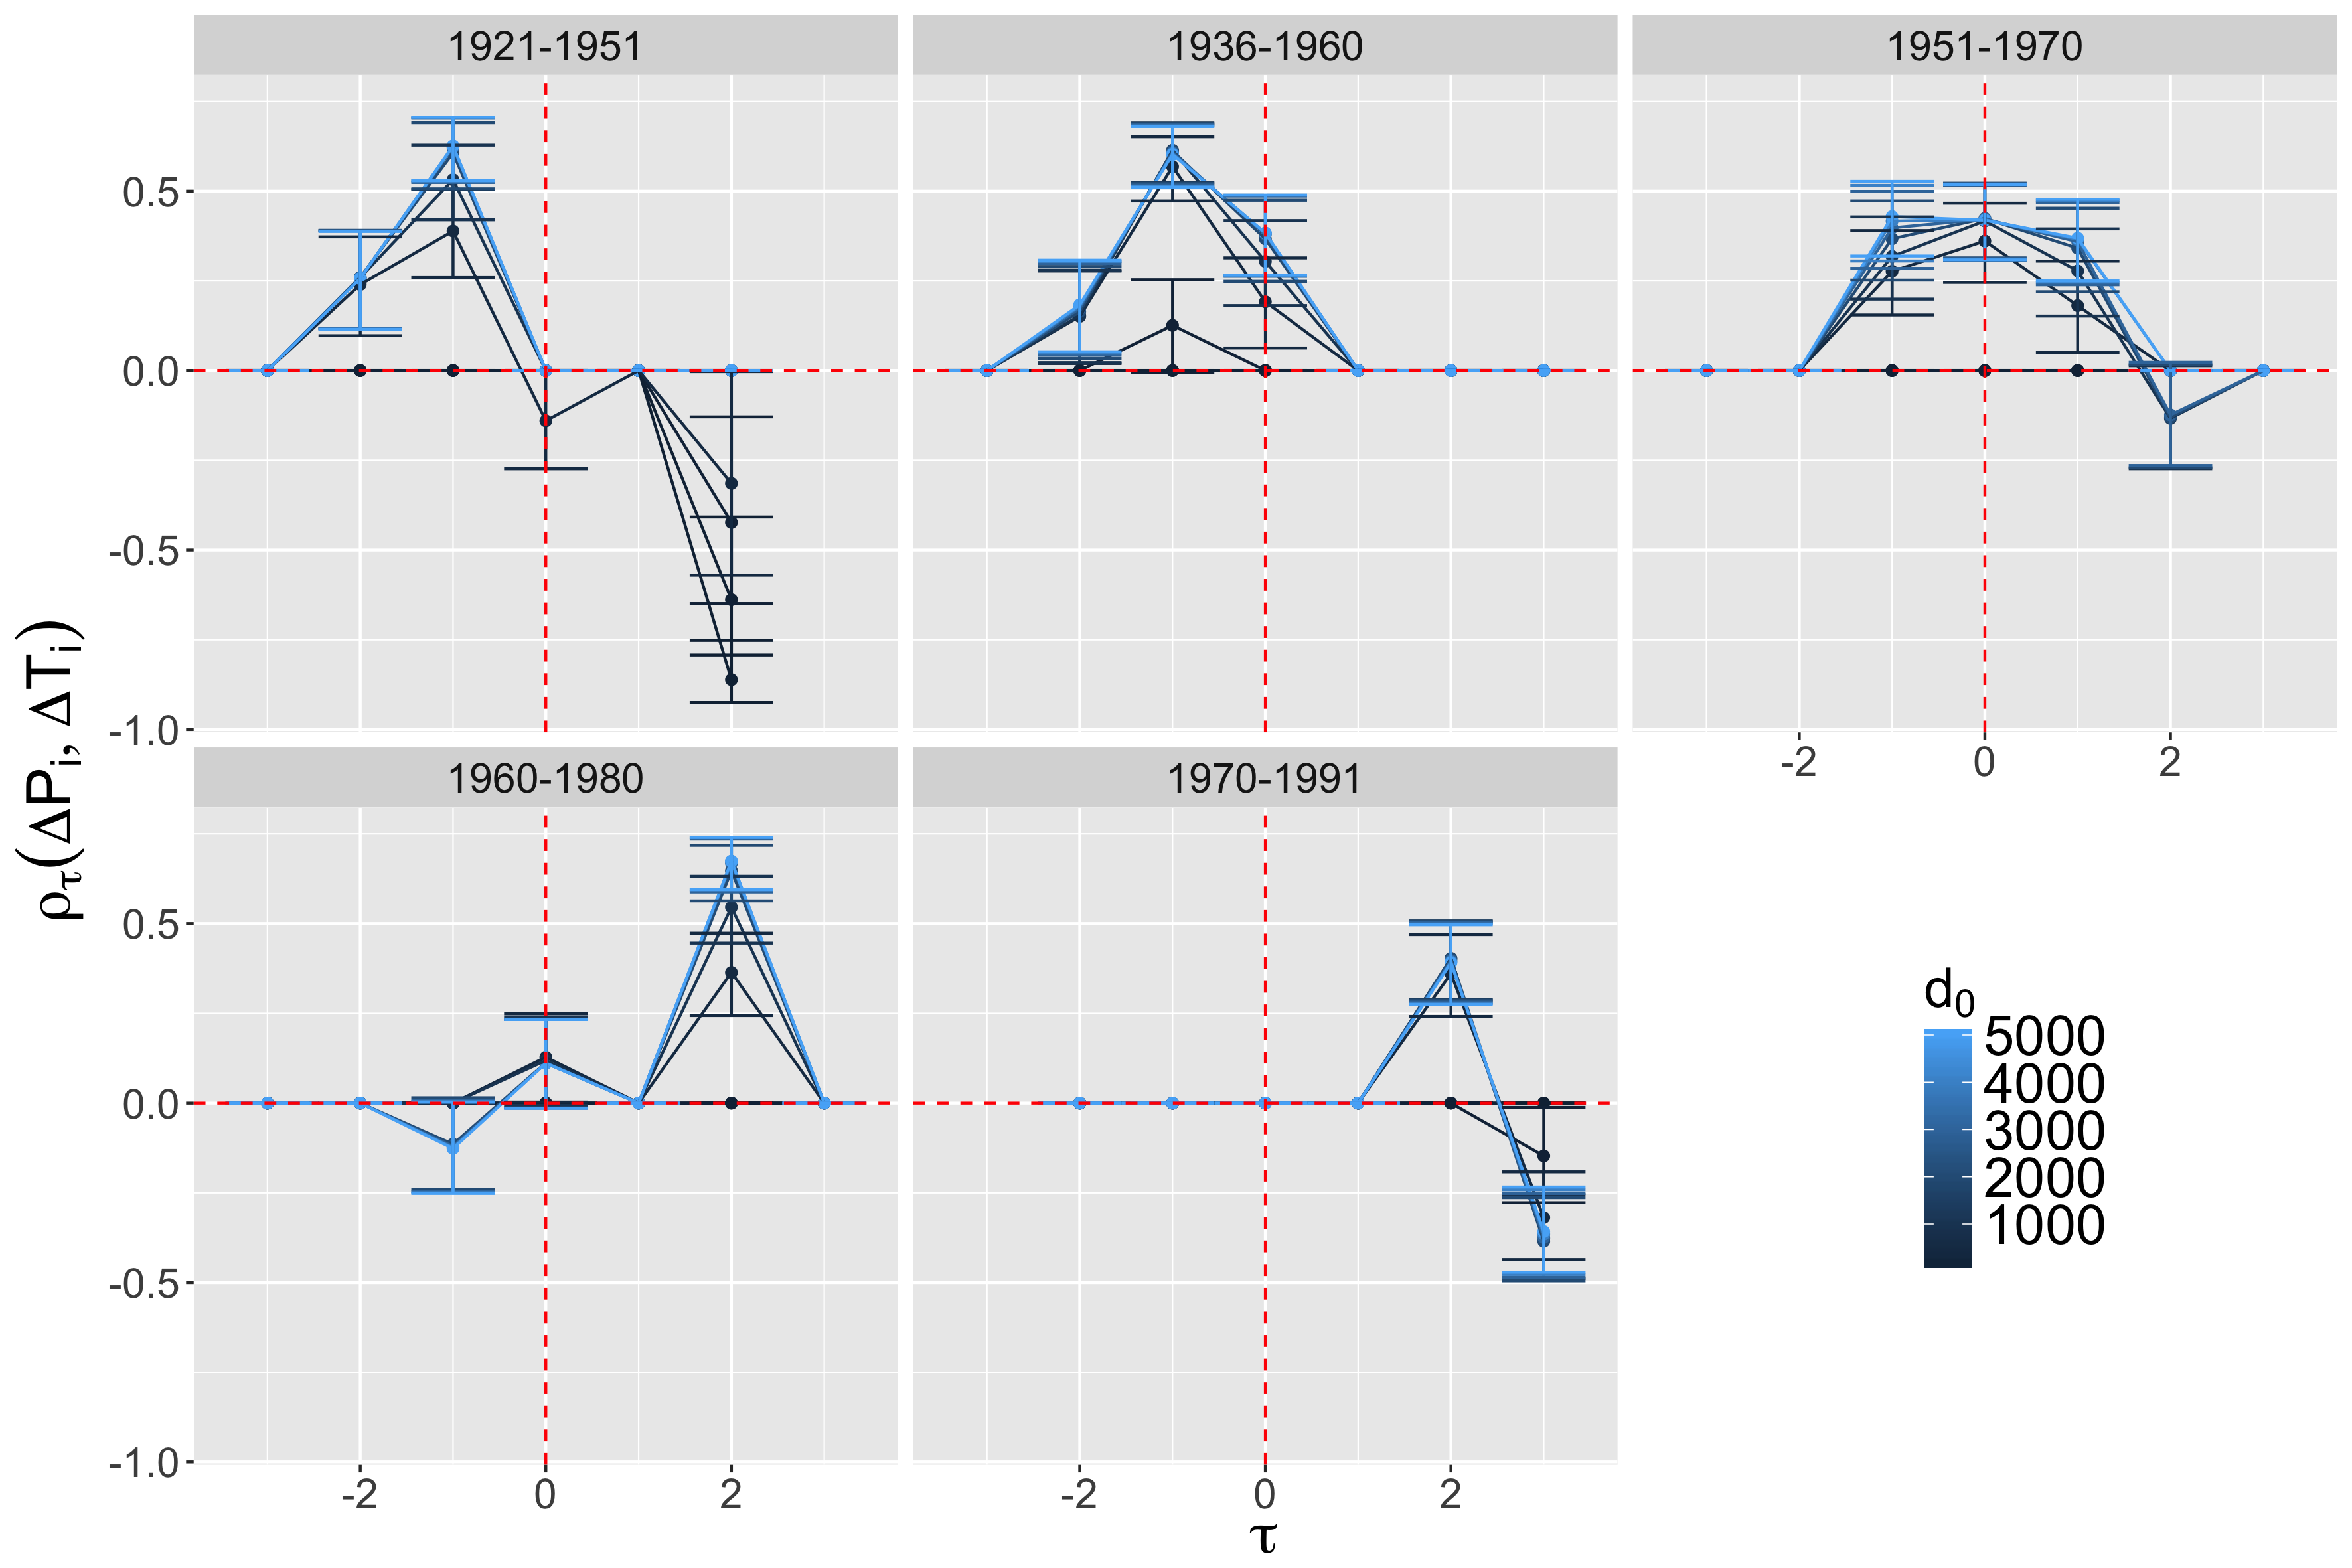
\includegraphics[width=\linewidth]{Figures/CausalityRegimes/laggedCorrs_time_Tw3.png}
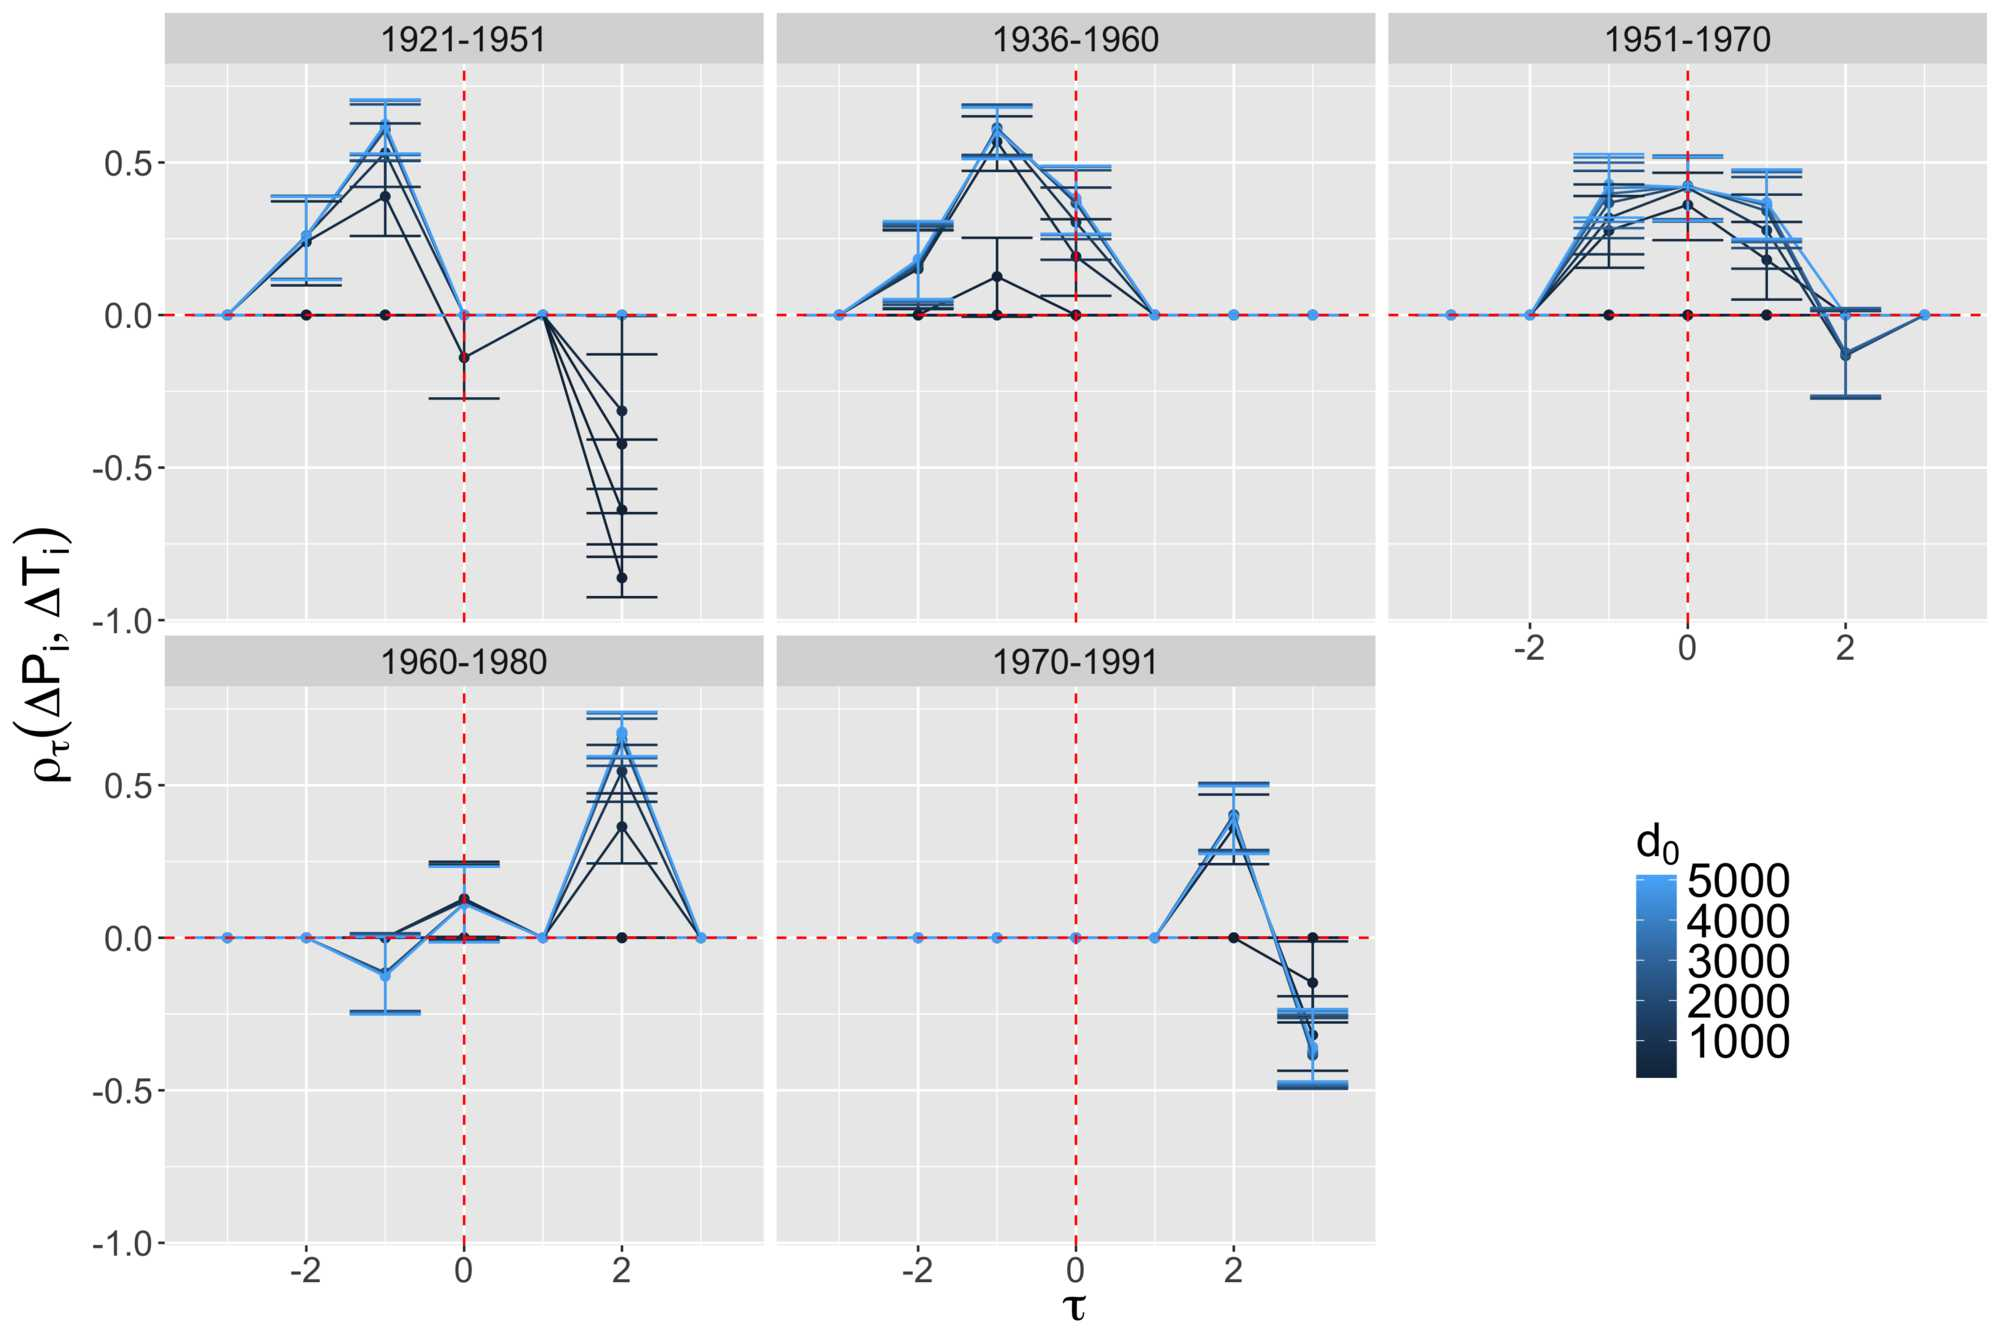
\includegraphics[width=\linewidth]{Figures/Final/4-2-3-fig-causalityregimes-sudafcorrs.jpg}
\caption[Lagged correlations in South Africa][Corrélations retardées entre croissance de population et gain d'accessibilité en Afrique du Sud]{\label{fig:causalityregimes:sudafcorrs}}{\textbf{Corrélations retardées.}  Corrélations retardées en fonction du délai $\tau$, pour la fenêtre temporelle $T_W=3$, sur les différentes périodes successives (colonnes), et pour $d_0$ variable (couleur). Pour interpréter, on observe un maximum de la corrélation retardée qui se décale dans le temps passant d'un retard négatif à un retard positif, ce qui selon notre définition correspond à une inversion du sens de la causalité.\label{fig:causalityregimes:sudafcorrs}}
\end{figure}
%%%%%%%%%%%%%%



\subsubsection{Possible developments}{Développements possibles}

\bpar{
Further work should consist in similar study with more precise socio-economic variables, for example quantifying directly segregation patterns. The method of instruments in statistics~\cite{angrist1996identification} is used to identify causal relationships between variables, in a different way than Granger causality test for example. Trying to identify causalities between network dynamics and territorial dynamics is of crucial importance to test our theoretical assumption on the existence of co-evolution.
}{
Une première extension pourra consister en une étude similaire avec des variables socio-économiques plus précises, pour quantifier par exemple directement les motifs de ségrégation. D'autre part, des variables qualitatives liées aux évènements historiques pourraient faire office de variable d'instrumentation. La méthode des variables instrumentales~\cite{angrist1996identification} est utilisée pour identifier des relations causales entre variables, d'une façon complémentaire à celle que nous avons mis en place. Nous pourrions chercher à rendre nos conclusions plus robustes, notamment vérifier si les corrélations ne sont pas fortuites, par l'application de cette approche, qui serait cependant difficile à réaliser vu la rareté des données dans notre cas.
}





\stars


% transition


Nous avons jusqu'ici dans ce chapitre exploré deux ingrédients de la théorie évolutive des villes, qui nous seront cruciaux pour comprendre la co-évolution entre réseaux de transport et territoires, à savoir les propriétés de non-stationnarité des corrélations, qui guideront la mise en place des modèles à une échelle similaire (chapitre~\ref{ch:morphogenesis} puis chapitre~\ref{ch:mesocoevolution}) et la possibilité de mise en évidence de régimes de causalité, qui nous servira d'outil de caractérisation de la co-évolution.

Nous proposons à présent d'introduire un dernier élément crucial de la théorie évolutive des villes, qui est l'appréhension des systèmes urbains par l'intermédiaire de modèles d'interaction entre villes. Ceux-ci ne seront pas co-évolutifs dans un premier temps mais leur ontologie visera à intégrer le rôle des réseaux dans le système urbain.



\stars





